\documentclass[12pt, a4paper]{article}

% Required Packages
\usepackage[utf8]{inputenc}
\usepackage{graphicx}
\usepackage{geometry}
\usepackage{fancyhdr}
\usepackage{hyperref}
\usepackage{subcaption}
\usepackage{float}
\usepackage{amsmath}

% Page Geometry
\geometry{top=1in, bottom=1in, left=1in, right=1in}

% Header and Footer Setup
\pagestyle{fancy}
\fancyhf{}
\rhead{12-Pulse LCC-HVDC System}
\lhead{Abd El-Rahman Muhammad Saad 19017058}
\cfoot{\thepage}

% Hyperlink Setup
\hypersetup{
    colorlinks=true,
    linkcolor=blue,
    filecolor=magenta,      
    urlcolor=blue,
}

\begin{document}

% ---------------- TITLE PAGE ---------------- %
\begin{titlepage}
    % Logo and University Name at the top left
    \begin{flushleft}
        \begin{minipage}{0.15\textwidth}
            
\includegraphics[width=\textwidth]{logo.png}
        \end{minipage}%
    \hspace{0.3cm}
        \begin{minipage}{0.7\textwidth}
            {\scshape\large Alexandria University} \\[0.1cm]
            {\scshape\normalsize Faculty of Engineering} \\[0.1cm]
            {\scshape\normalsize Electrical Engineering Department}
        \end{minipage}
    \end{flushleft}
    
    \vspace{2.0cm}
    \centering
    {\Huge\bfseries HVDC Transmission System \par}
    \vspace{0.4cm}
    {\Large\bfseries 12-Pulse LCC-HVDC System: Control and Fault Analysis 	 \par}
    
    \vspace{1.0cm}
    % --- Extra Academic Details ---
    {\Large\itshape Prepared by:\par}
    \vspace{0.2cm}
    {\Large \textbf{Abd El-Rahman Muhammad Saad Muhammad}\par}
    {\large \textbf{ID:} 19017058\par}
    
    \vspace{1.2cm}
    {\Large\itshape Submitted to:\par}
    \vspace{0.2cm}
    {\Large \textbf{Prof. Ahmed El-Serougi}\par}
    
    \vspace{1.5cm}
    {\large \textbf{Simulink Model Link:}\par}
    {\normalsize \href{https://github.com/Abd-El-Rhman-Saad/hvdc-12pulse-lcc-simulation.git}{Click here to access the Simulink Model on GitHub}}\par
    
    \vfill
    {\large \textbf{Date:} April 25, 2026 \par}
\end{titlepage}

\newpage

\begin{abstract}
	This report presents the modeling and simulation of a 1.56 GW, 200 kV 12-pulse Line-Commutated Converter (LCC) HVDC transmission system. The study evaluates the system's dynamic performance under normal operating conditions utilizing Constant Current (CC) and Constant Extinction Angle (CEA) control strategies. Furthermore, the system's resilience is tested under a severe 25\% AC voltage sag at the rectifier side, demonstrating a successful automated control handover mechanism to Constant Ignition Angle (CIA) and Inverter CC mode.
\end{abstract}

\newpage
% -------------- TABLE OF CONTENTS -------------- %
\tableofcontents
\newpage

\section{System Specifications}
The system parameters utilized for the simulation are derived from the project requirements and are detailed in Table 1.

\begin{table}[H]
	\centering
	\caption{HVDC System Simulation Parameters}
	\begin{tabular}{lc}
		\hline
		\textbf{Parameter} & \textbf{Value} \\
		\hline
		Rated Power & 1.56 GW \\
		DC Link Voltage & +200 kV \\
		DC Line Resistance & $5\,\Omega$ \\
		Bus A (Rectifier) AC Voltage & 75.19 kV (rms) \\
		Bus B (Inverter) AC Voltage & 77.618 kV (rms) \\
		System Frequency & 50 Hz \\
		\hline
	\end{tabular}
\end{table}

% ========================================================= %
% ----------------------- CASE A -------------------------- %
% ========================================================= %
\section{Case A: Normal Operating Conditions}
In this scenario, the HVDC transmission system operates under steady and balanced grid conditions, aiming to maintain a nominal target DC voltage of 200 kV. The coordination between the two converter stations relies on a robust dual-terminal control strategy, which is the standard industry practice for LCC-HVDC links. The Rectifier station acts as the primary current regulator, employing a Constant Current (CC) control loop. It continuously adjusts its firing angle ($\alpha$) to minimize the error between the measured DC link current and the dynamic reference signal. 

Conversely, the Inverter station operates under Constant Extinction Angle (CEA) control. It maintains the extinction angle ($\gamma$) at a safe predetermined value (typically $40^{\circ}$) to establish the DC voltage profile and provide a sufficient margin to prevent commutation failures. Furthermore, this case evaluates the system's dynamic tracking capability by applying sudden step changes to the current reference, observing the response of the PI controllers.

\subsection{System Configuration (Case A)}
Figure 1 illustrates the internal subsystems utilized during normal operation, detailing the original wiring and control logic before any grid faults are introduced. The configuration prominently features 12-pulse thyristor converters at both ends to significantly mitigate 5th and 7th AC harmonic distortions. The control circuits are equipped with Proportional-Integral (PI) controllers meticulously tuned to deliver a fast dynamic response with minimal overshoot.

\begin{figure}[H]
    \centering
    \begin{subfigure}{0.48\textwidth}
        \centering
        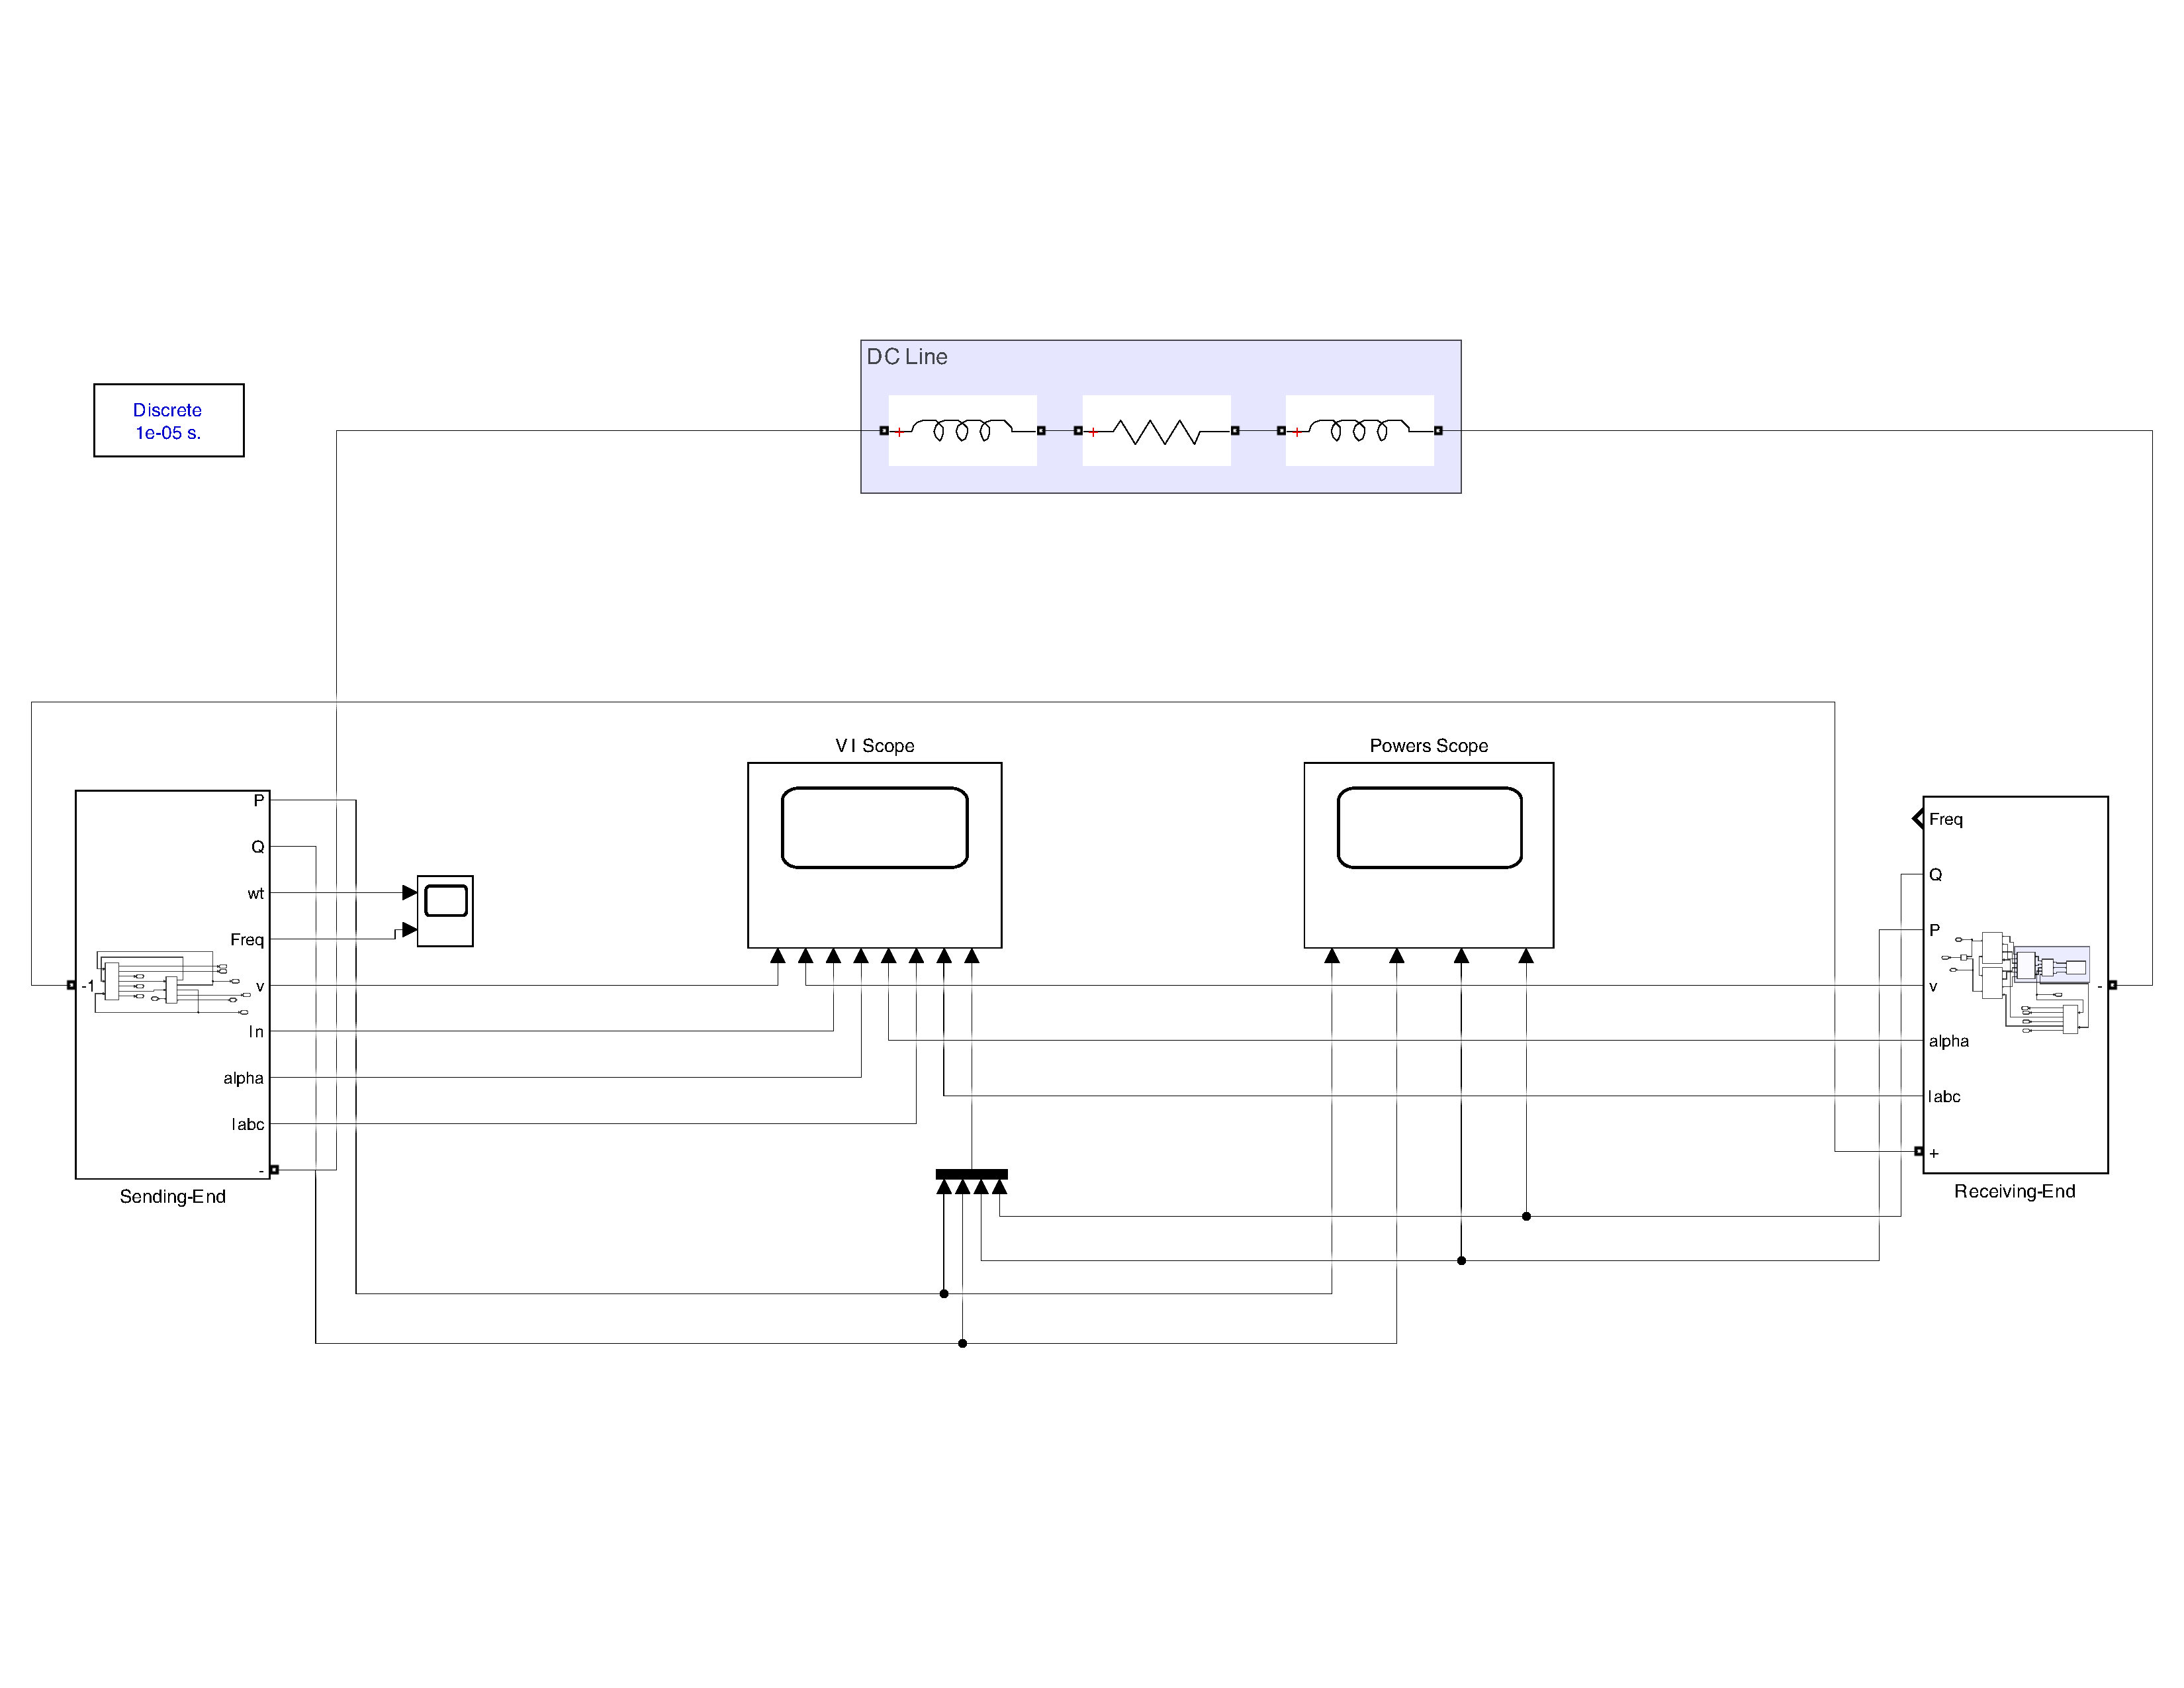
\includegraphics[width=\textwidth]{A_sys1.jpg}
        \caption{\textbf{Main System:} Overall architecture.}
    \end{subfigure}
    \hfill
    \begin{subfigure}{0.48\textwidth}
        \centering
        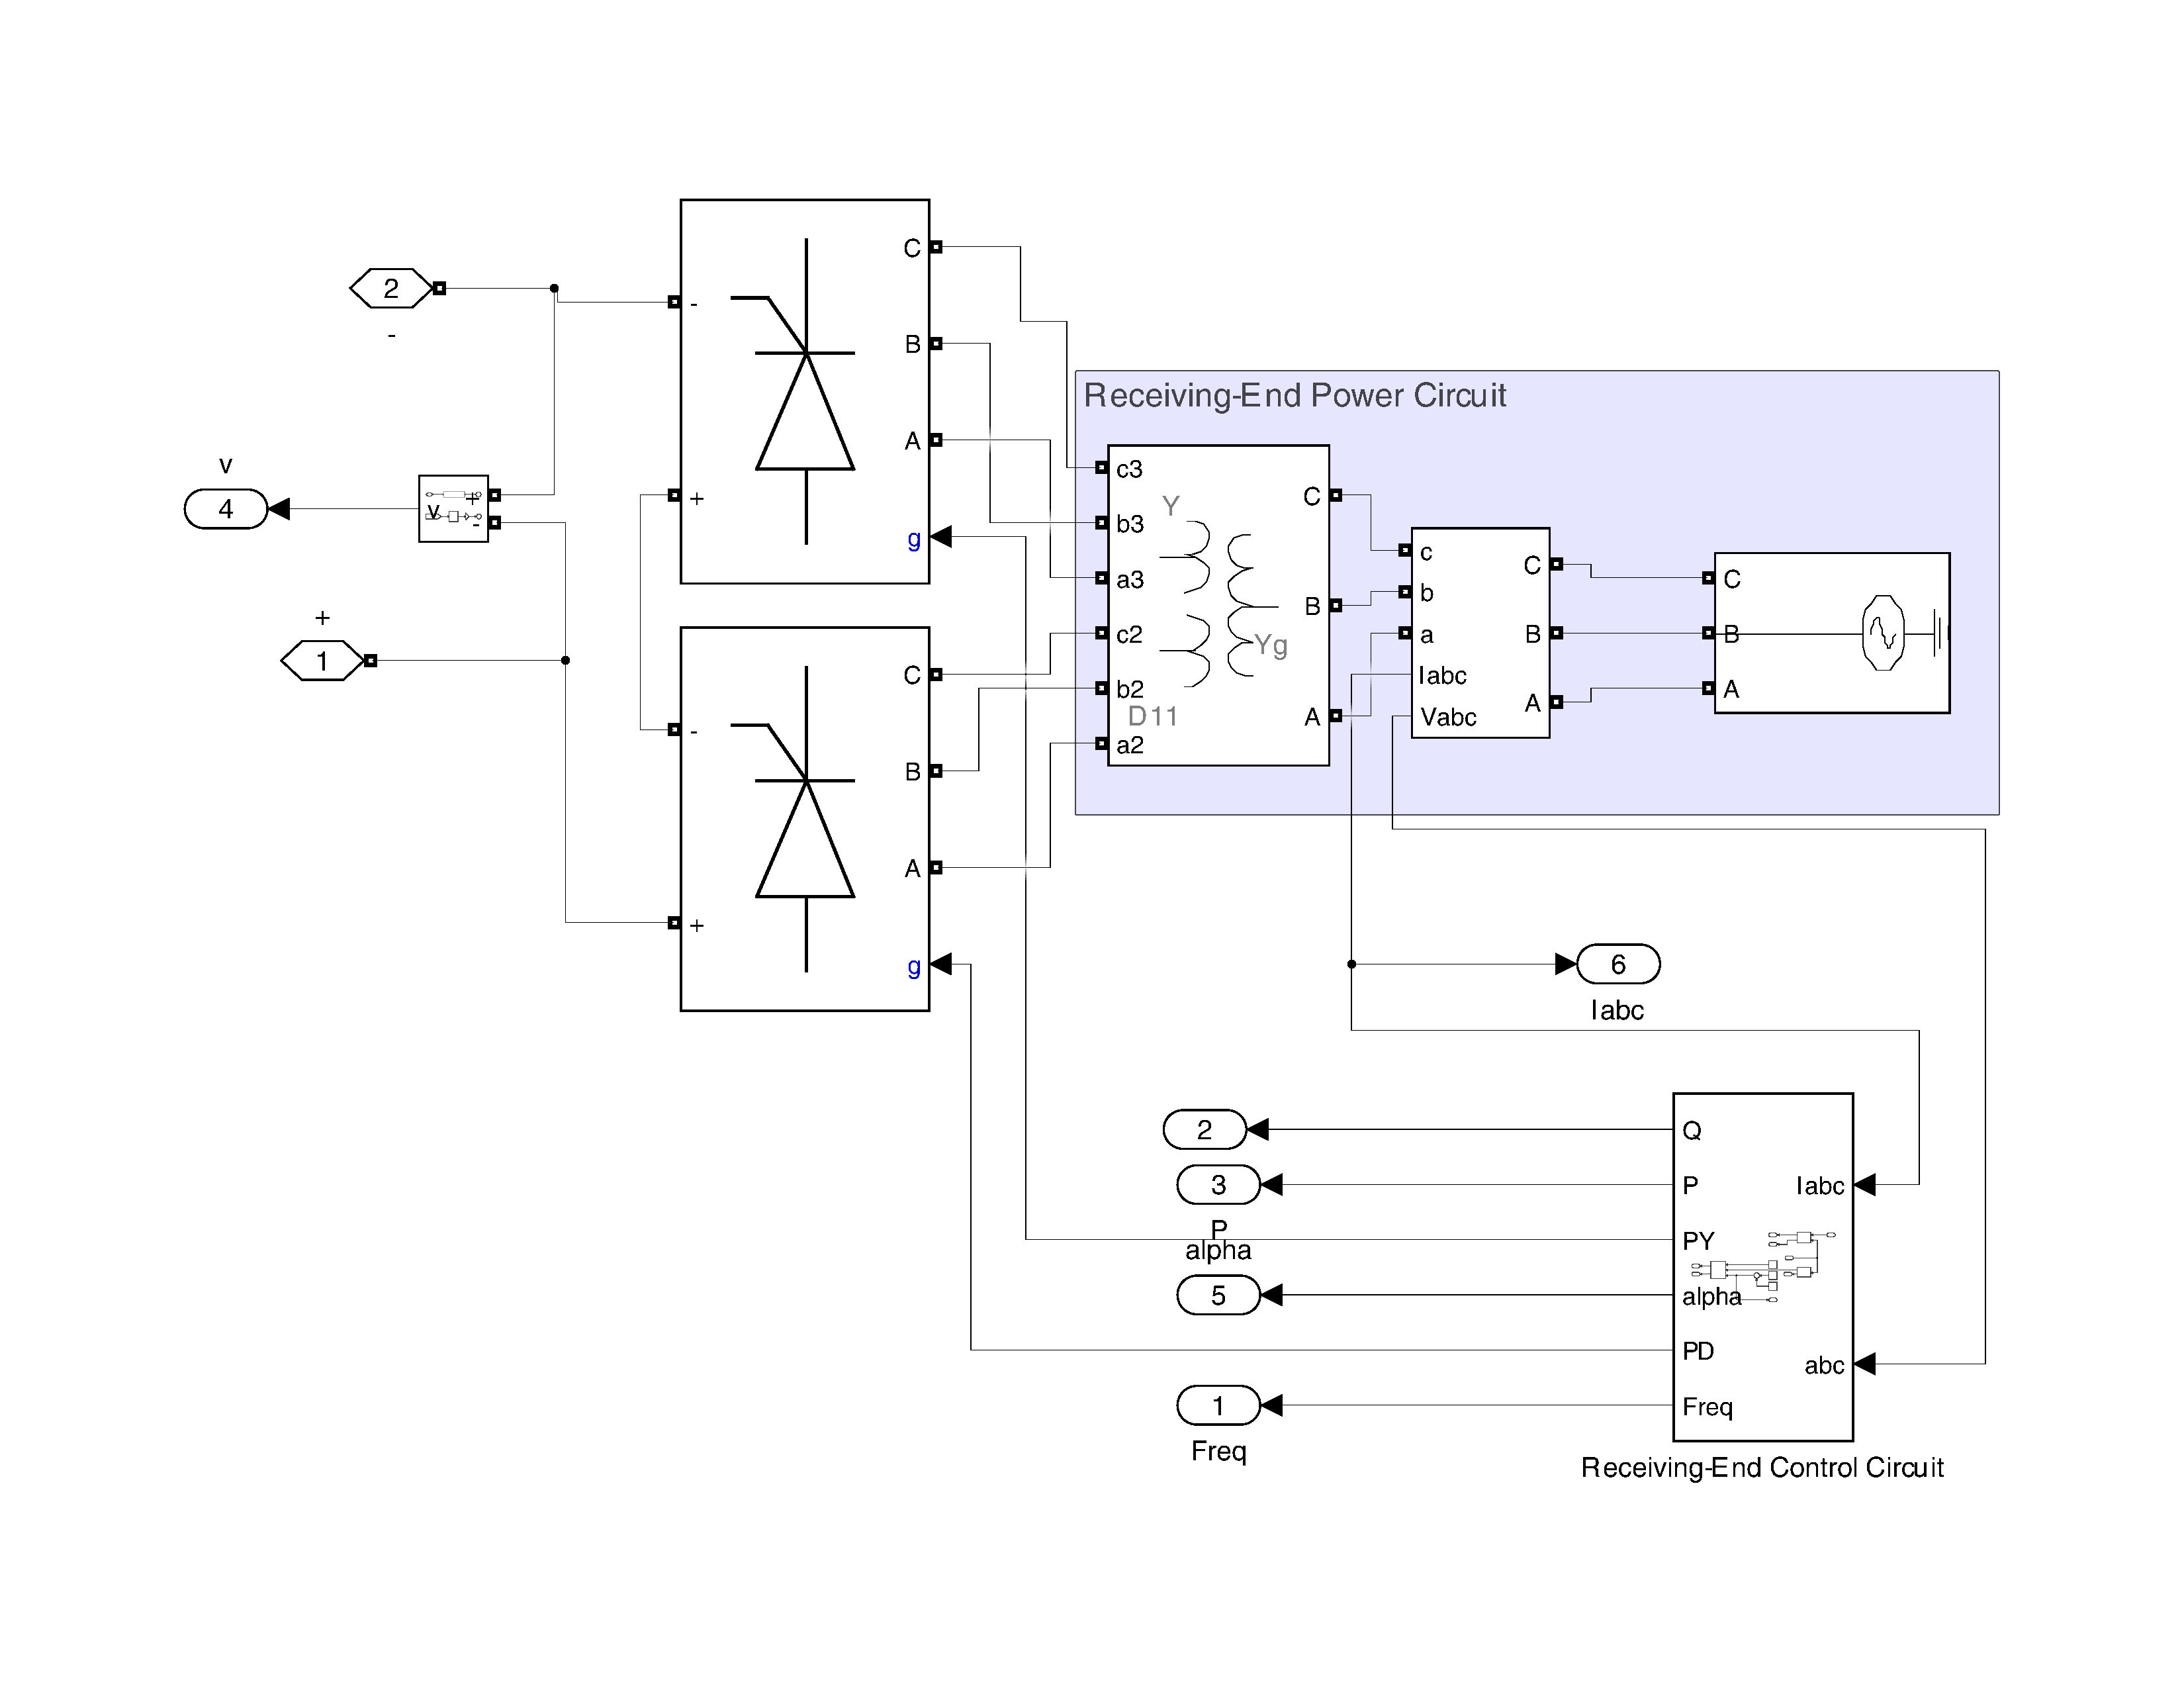
\includegraphics[width=\textwidth]{A_sys2.jpg}
        \caption{\textbf{Receiving Power Circuit:} Transformer and bridges.}
    \end{subfigure}
    
    \vspace{0.3cm}
    \begin{subfigure}{0.48\textwidth}
        \centering
        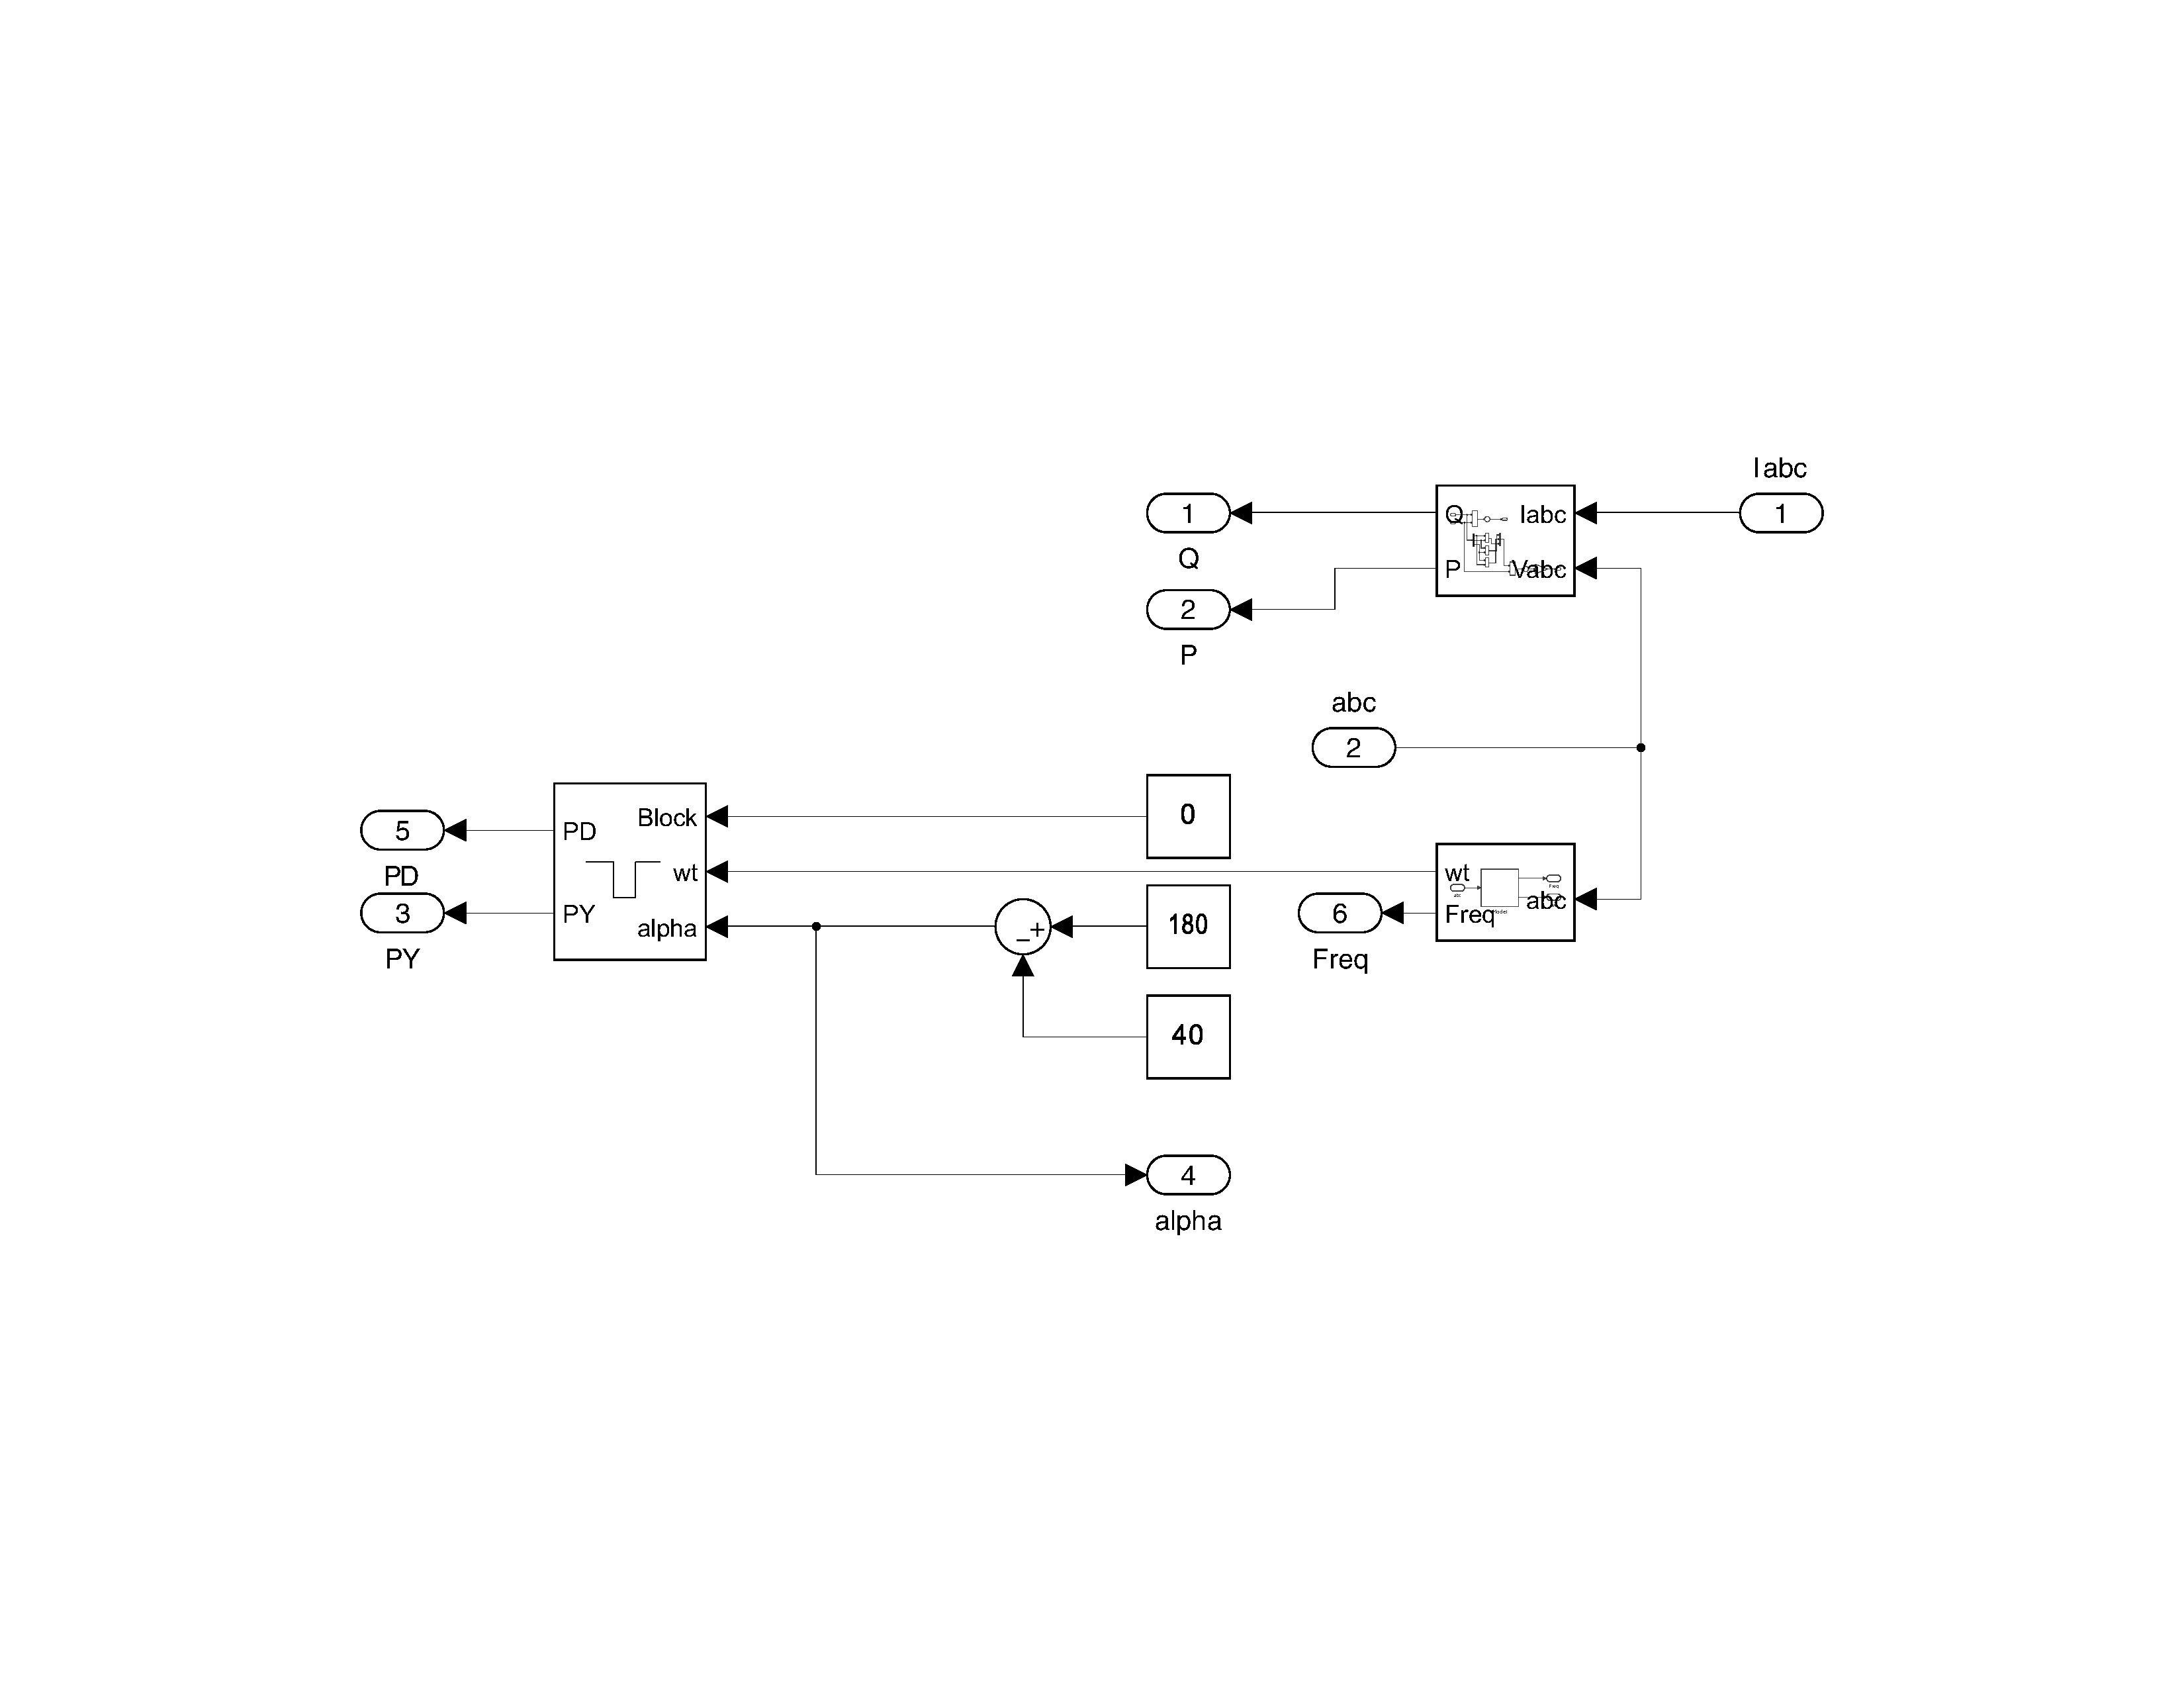
\includegraphics[width=\textwidth]{A_sys3.jpg}
        \caption{\textbf{Receiving Control Circuit:} Original CEA logic.}
    \end{subfigure}
    \hfill
    \begin{subfigure}{0.48\textwidth}
        \centering
        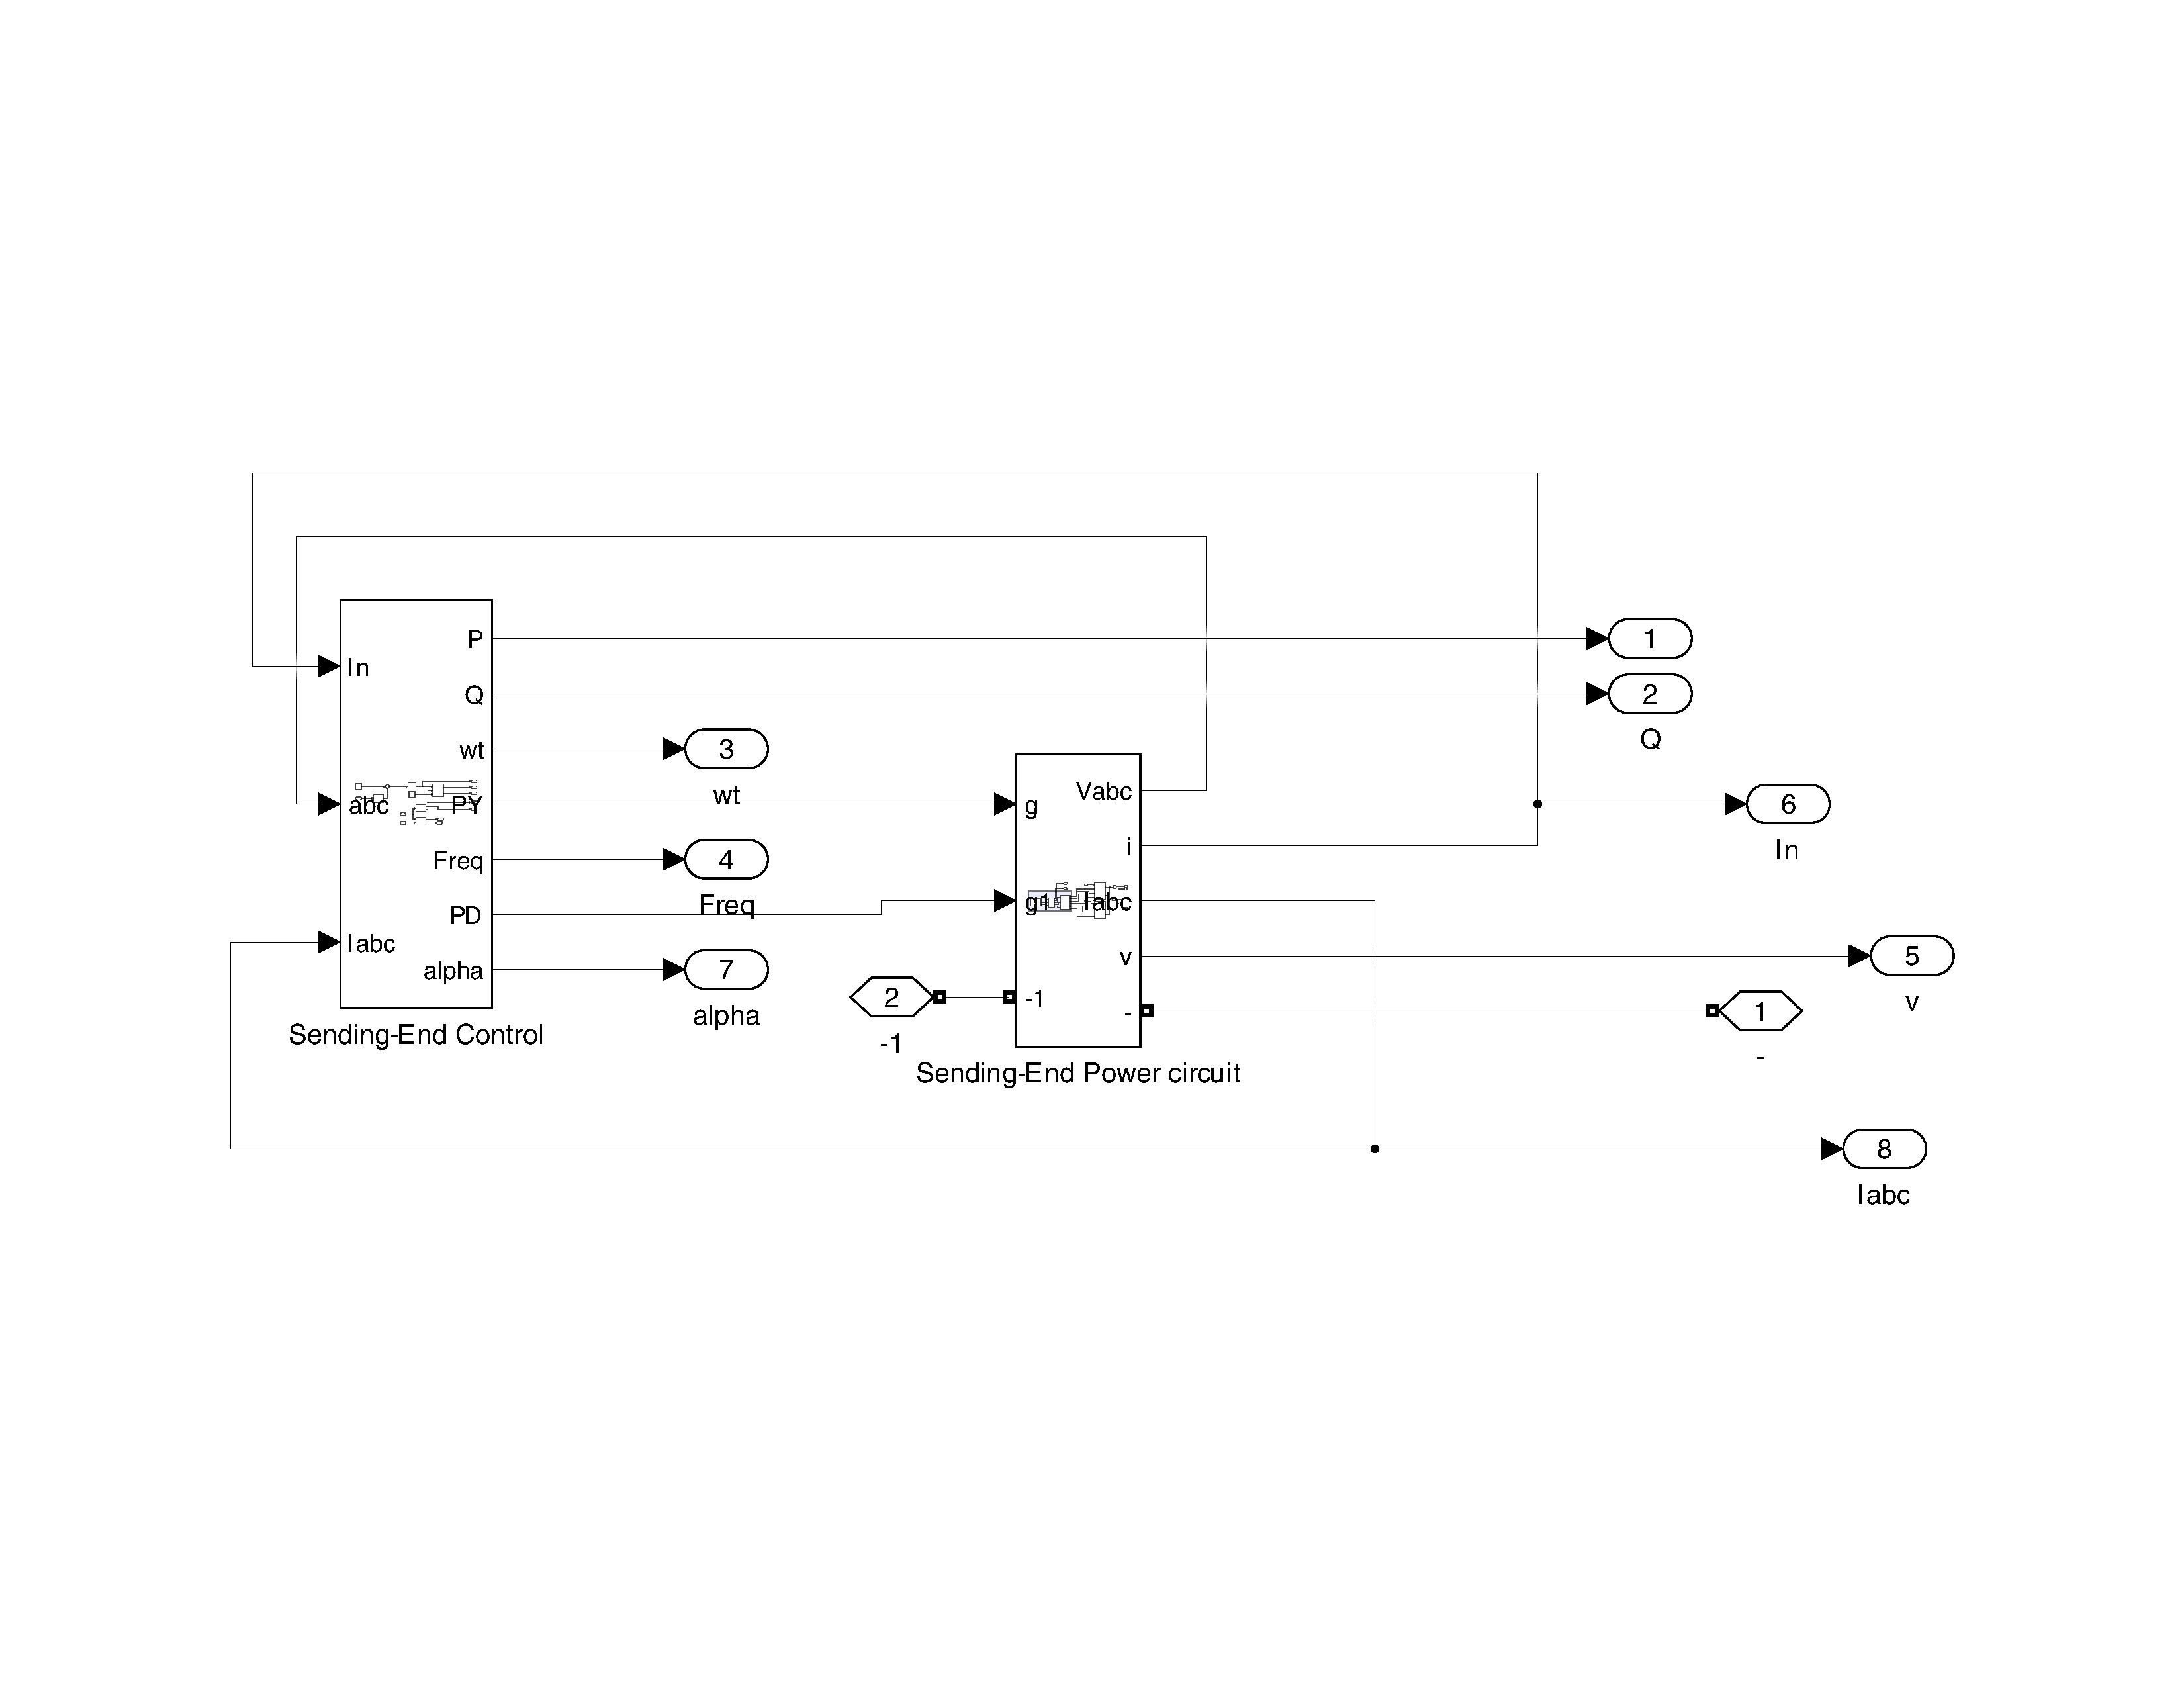
\includegraphics[width=\textwidth]{A_sys4.jpg}
        \caption{\textbf{Sending Control Circuit:} CC control logic.}
    \end{subfigure}
    
    \vspace{0.3cm}
    \begin{subfigure}{0.48\textwidth}
        \centering
        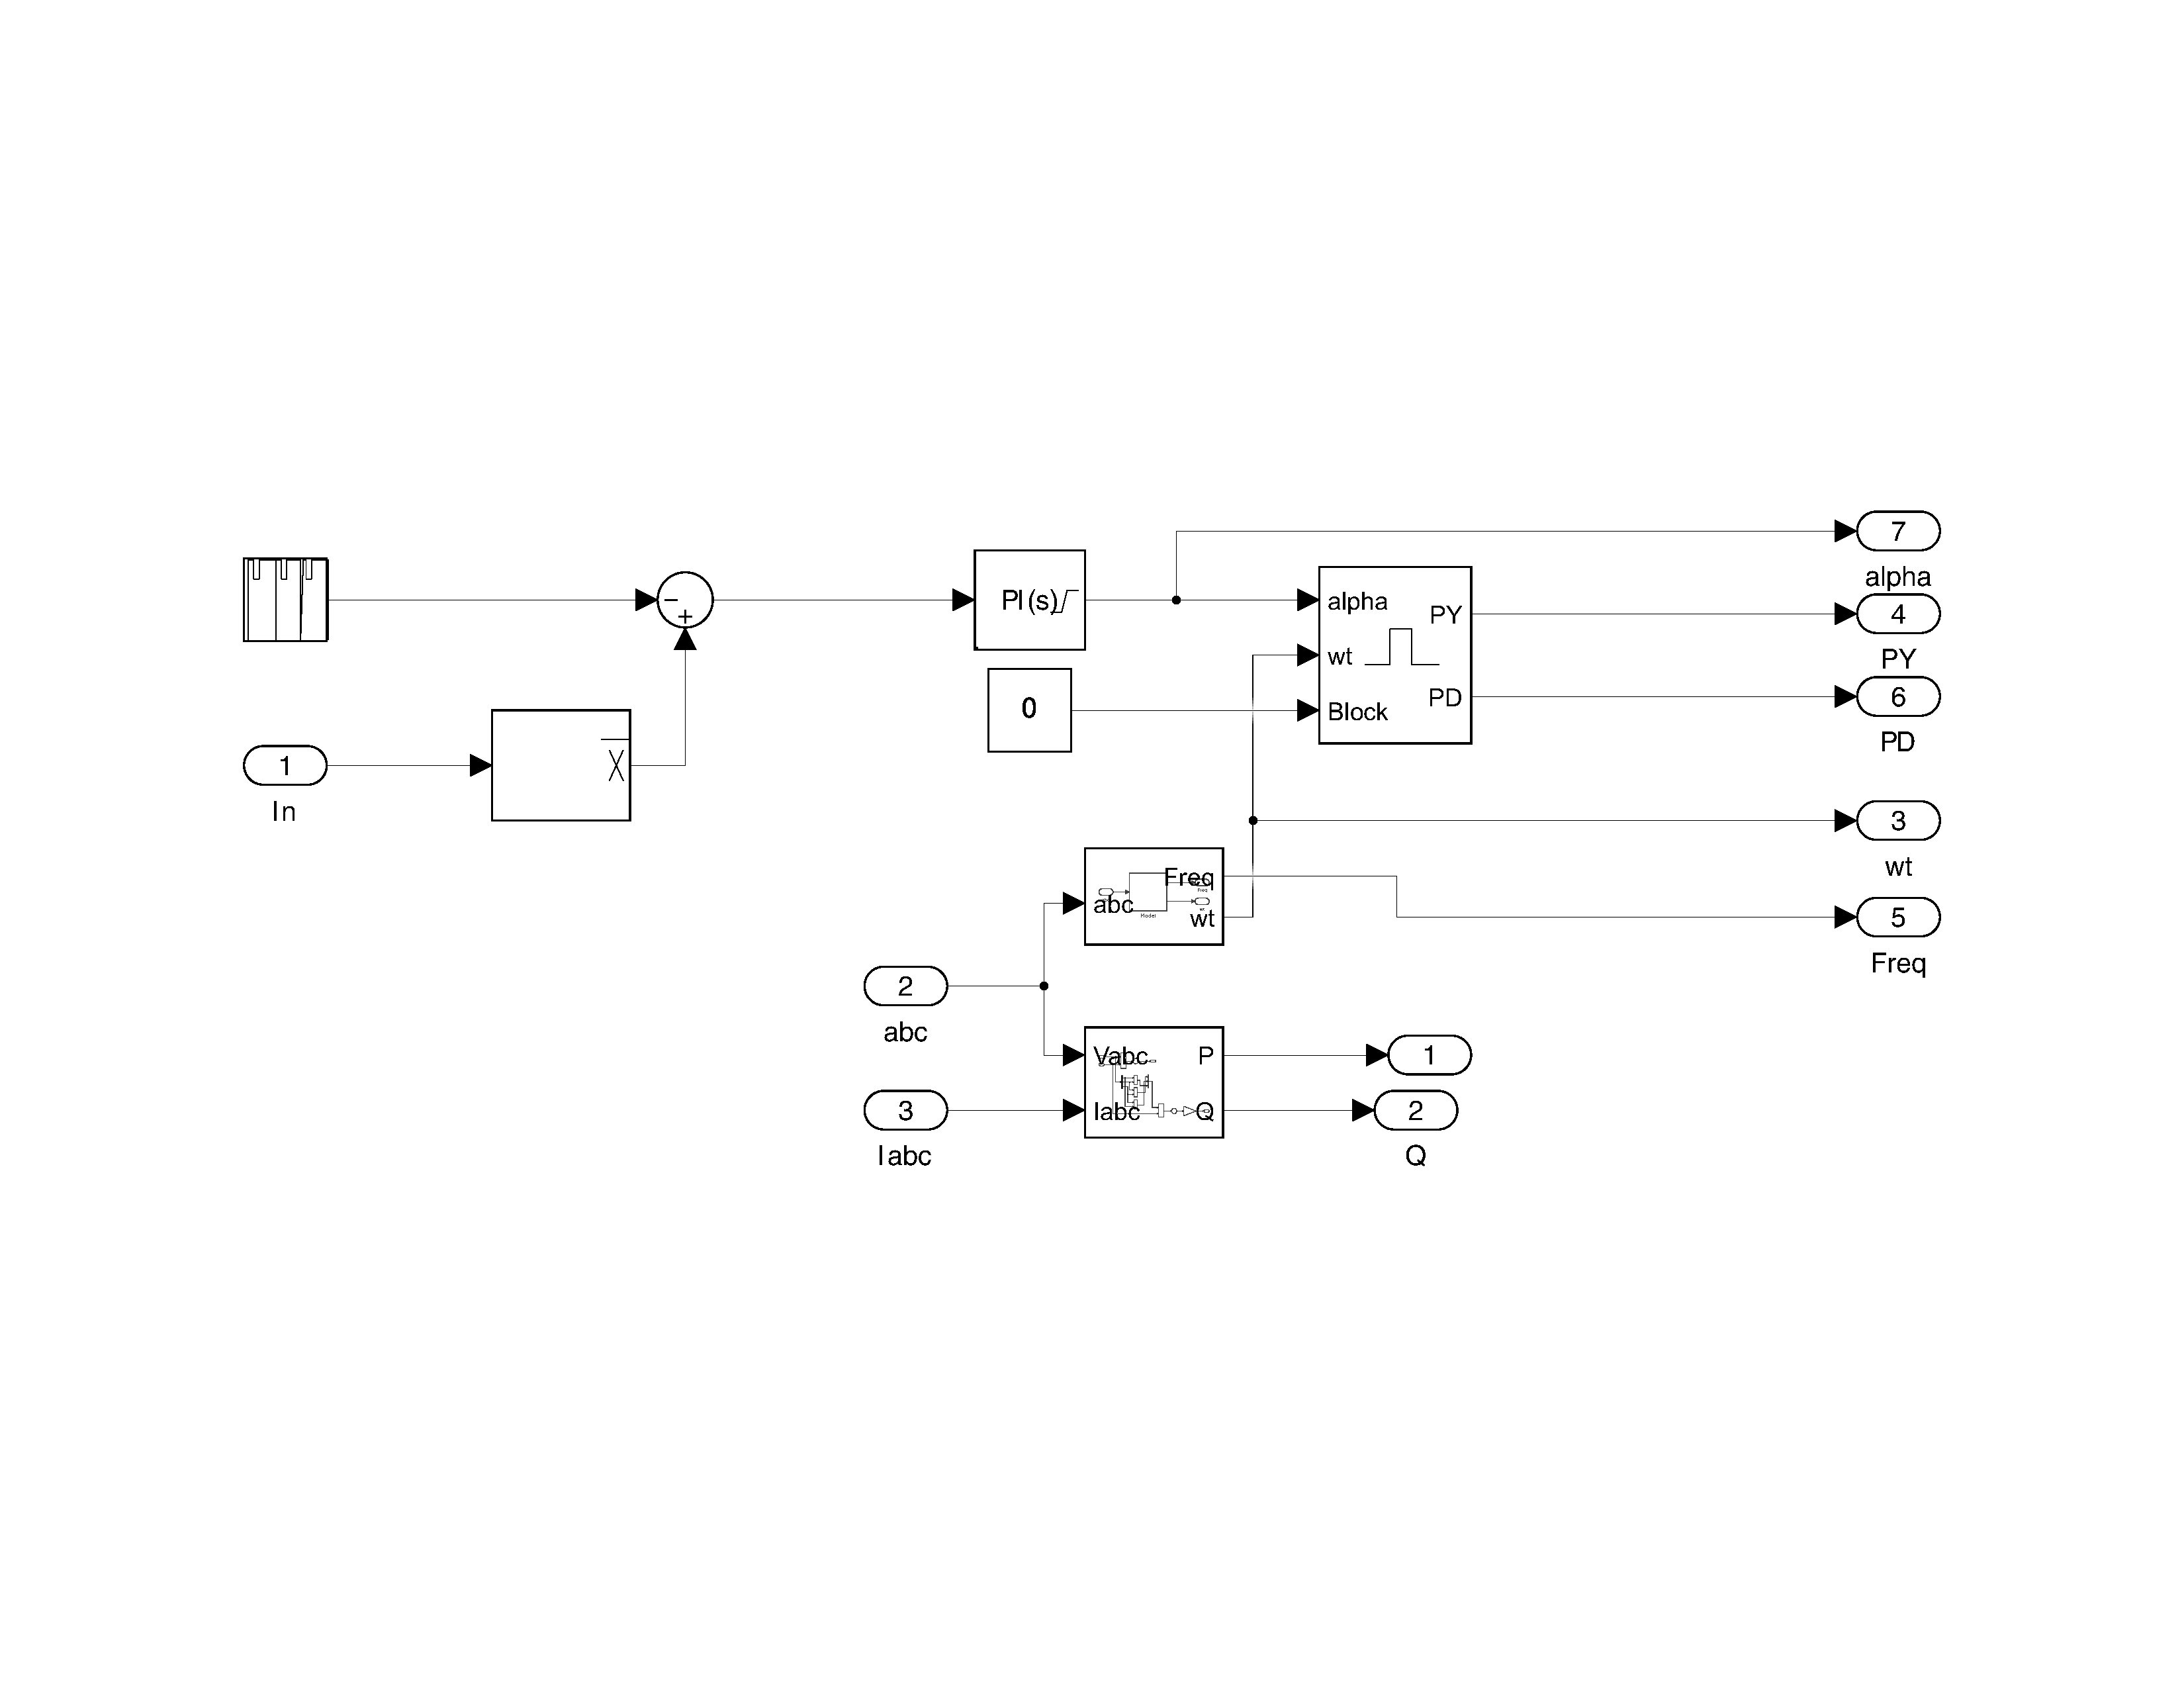
\includegraphics[width=\textwidth]{A_sys5.jpg}
        \caption{\textbf{Pulse Generator Unit:} Synchronization block.}
    \end{subfigure}
    \hfill
    \begin{subfigure}{0.48\textwidth}
        \centering
        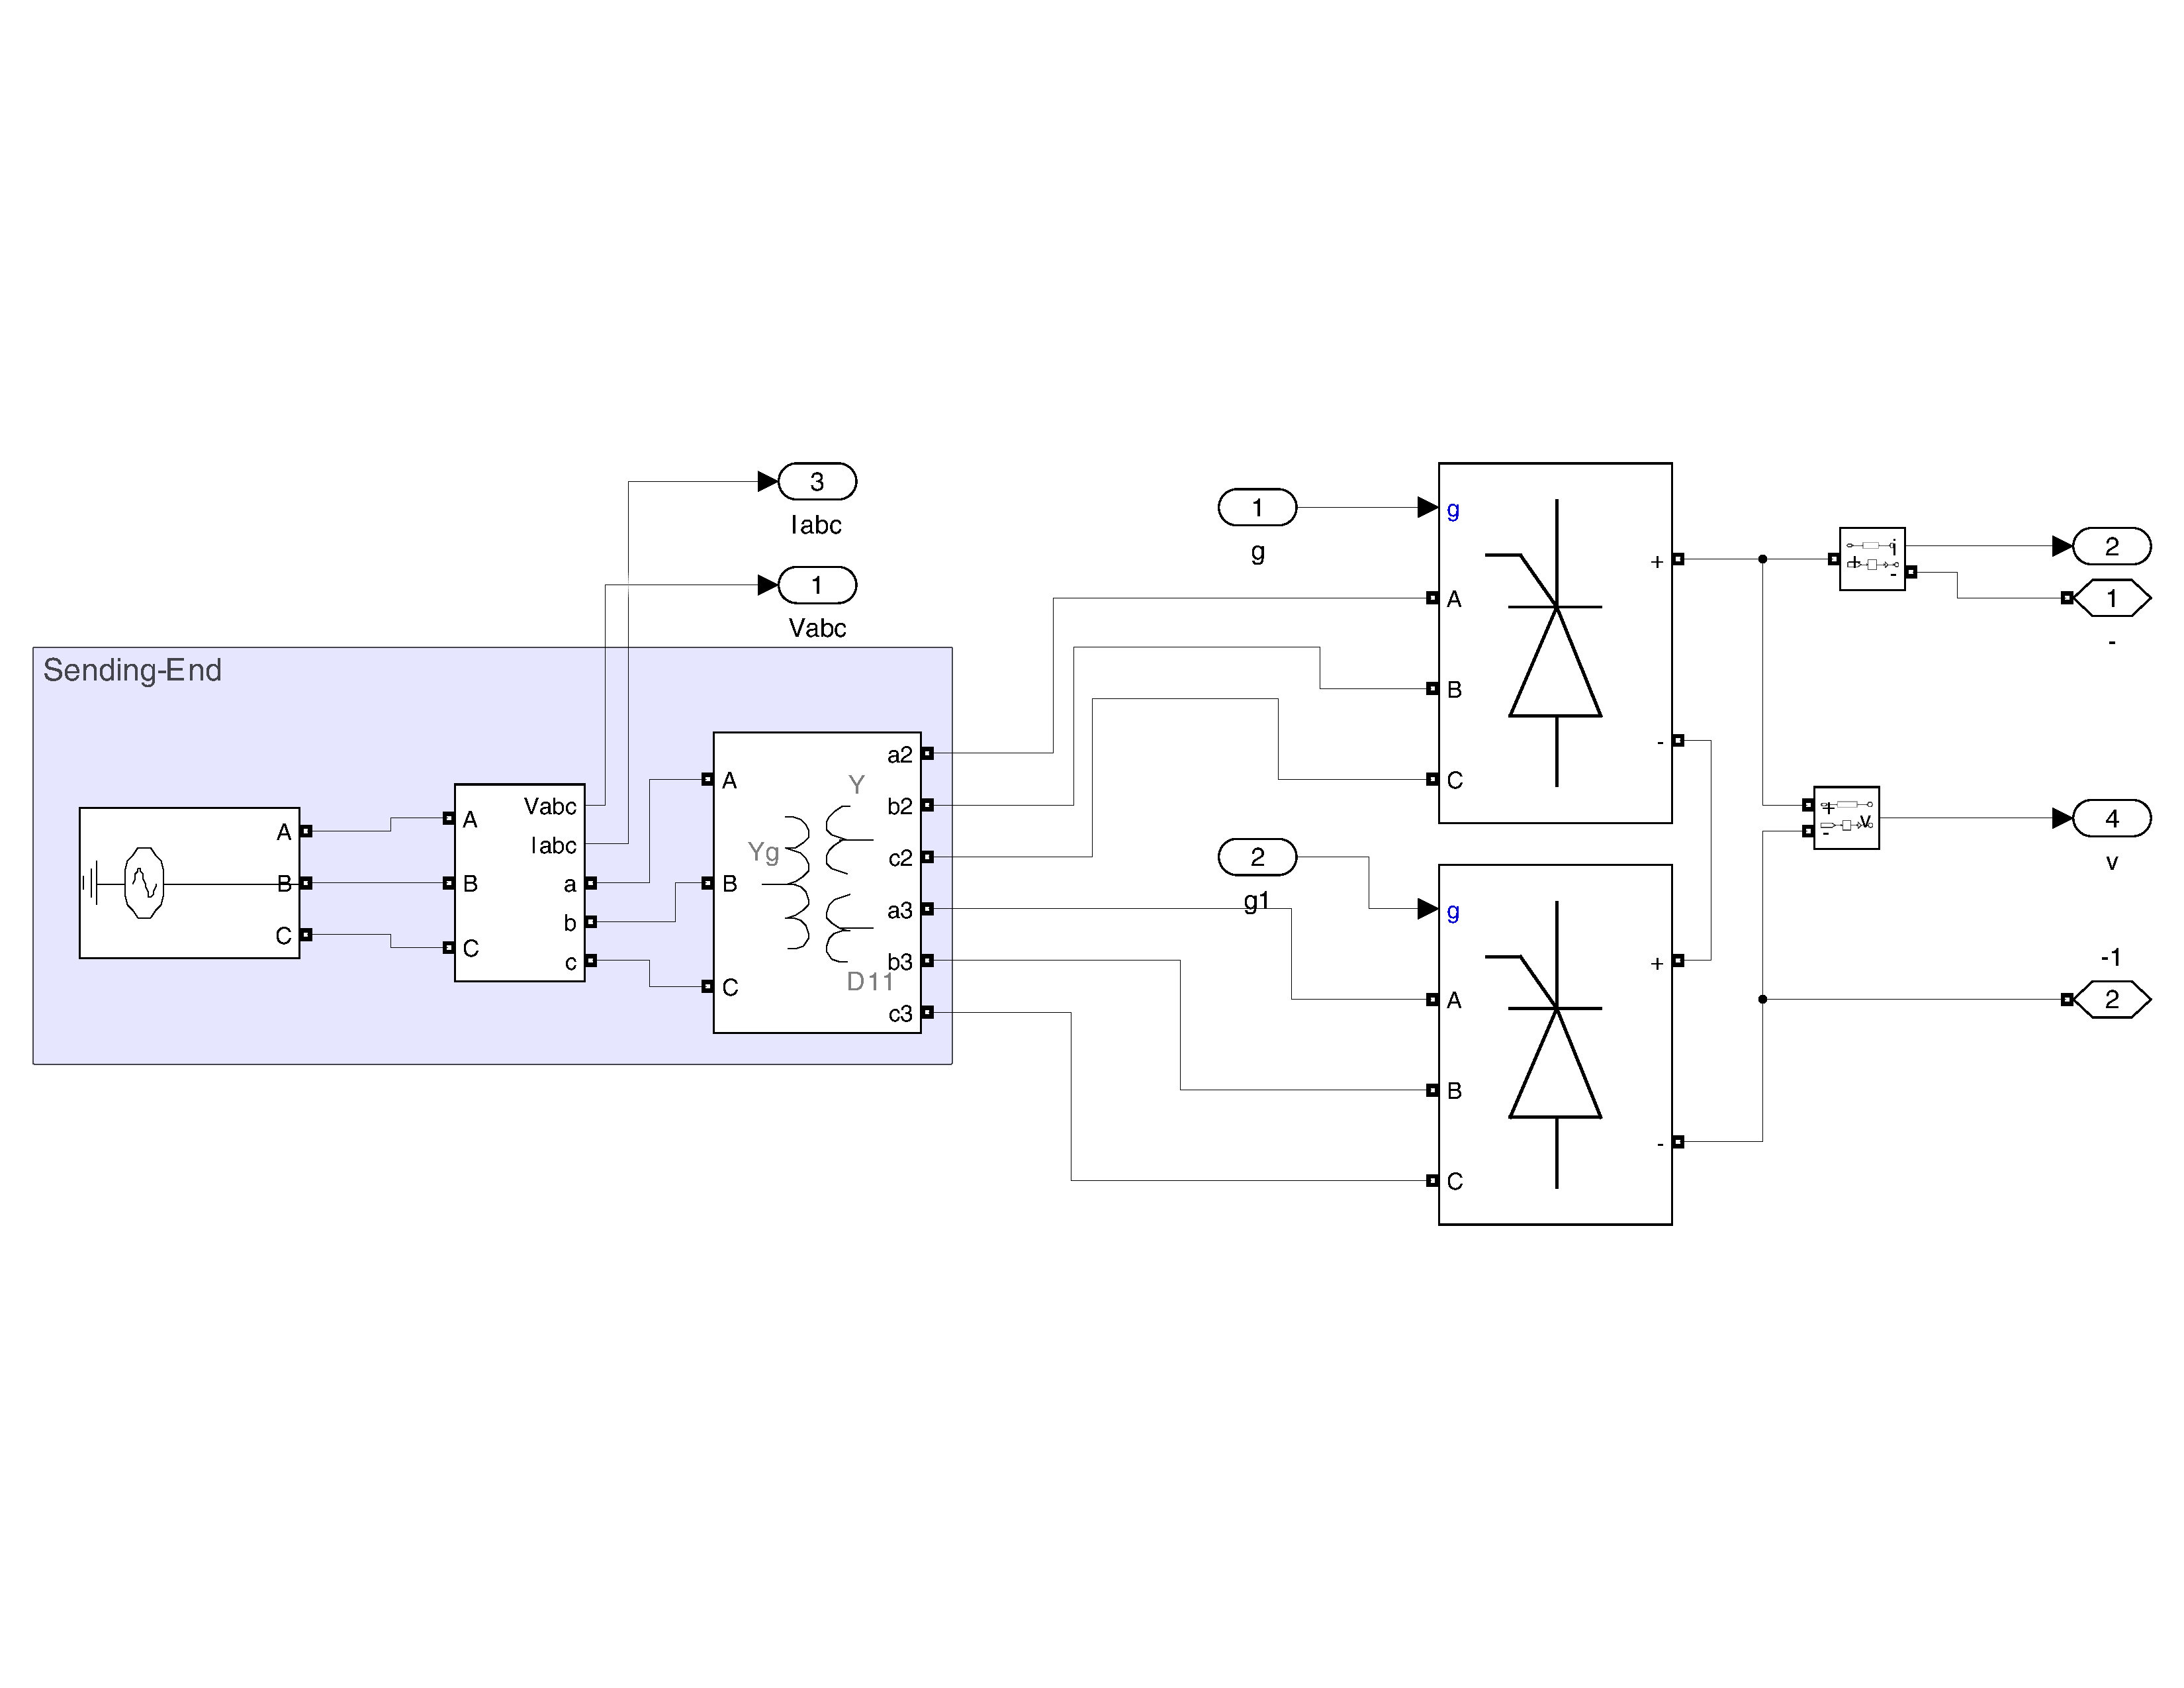
\includegraphics[width=\textwidth]{A_sys6.jpg}
        \caption{\textbf{Sending Power Circuit:} Rectification bridges.}
    \end{subfigure}
    \caption{Subsystem Configurations for Case A (Normal Operation).}
\end{figure}

\newpage
\subsection{Overall System Performance (Case A)}
Figures 2 and 3 display the combined scopes of the system's dynamic response to step changes in the current reference.

\begin{figure}[H]
    \centering
    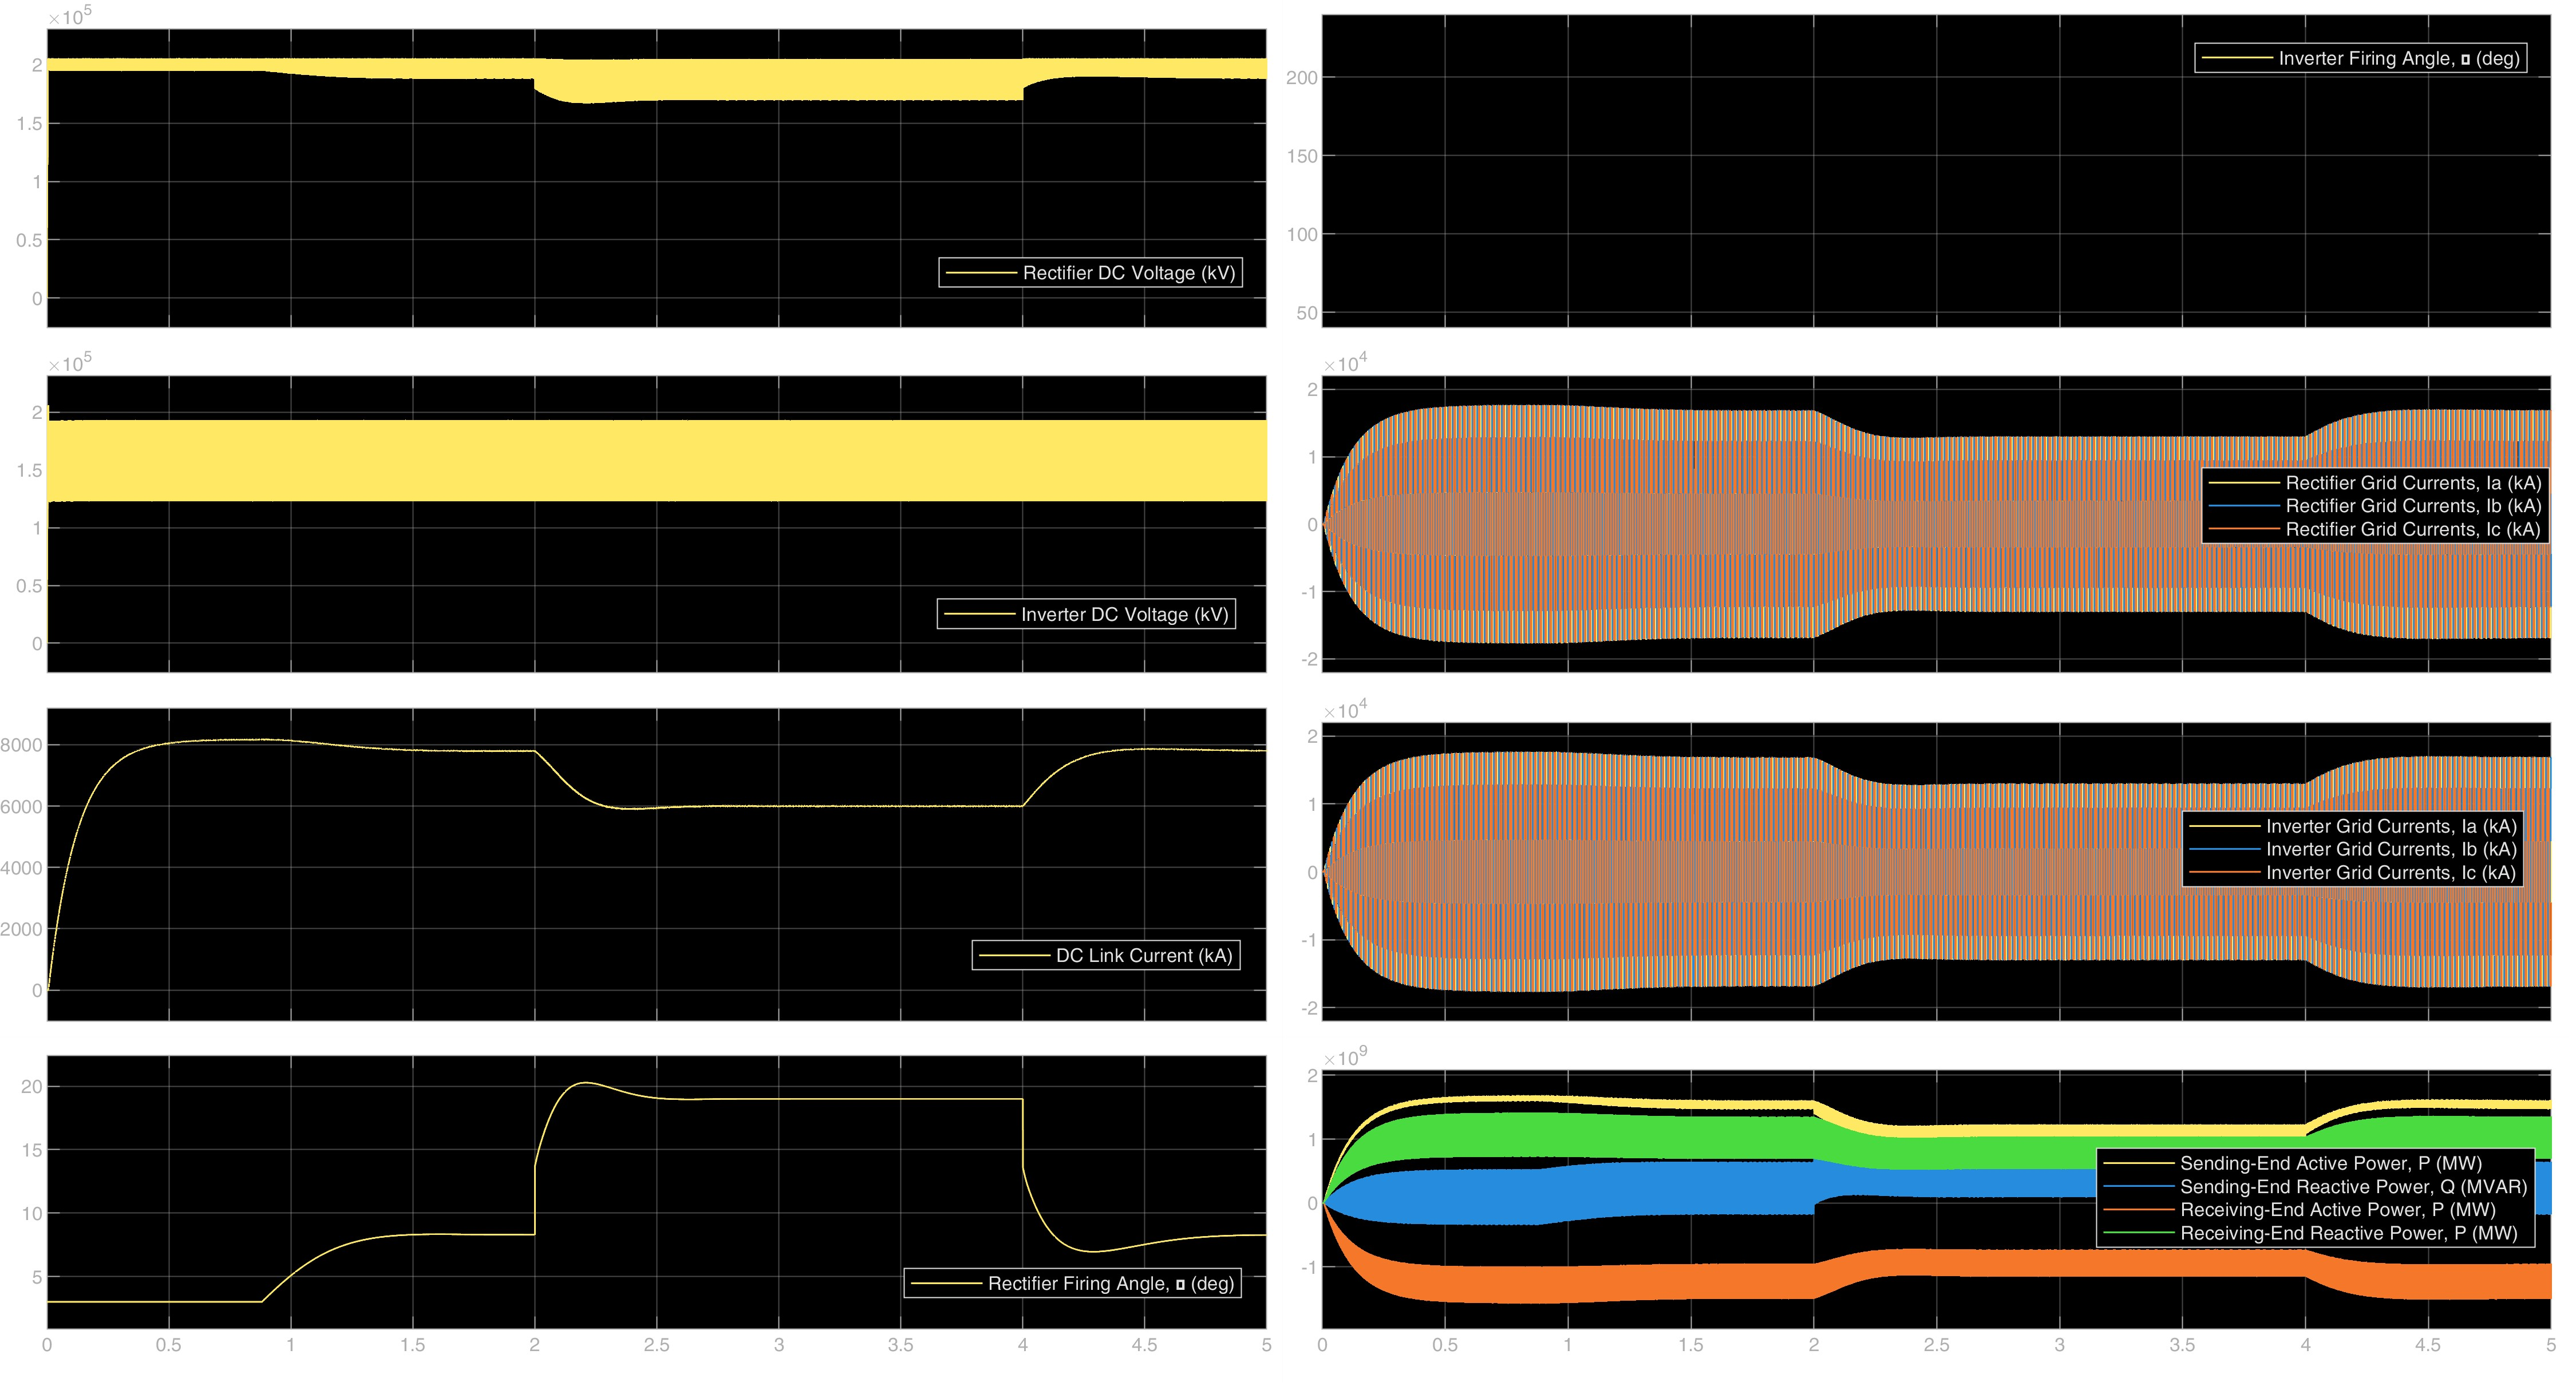
\includegraphics[width=0.95\textwidth]{A_VI.jpg}
    \caption{\textbf{VI Scope:} Displays the synchronization between voltages, currents, and firing angles as the system accurately tracks the step references under normal grid conditions.}
\end{figure}

\begin{figure}[H]
    \centering
    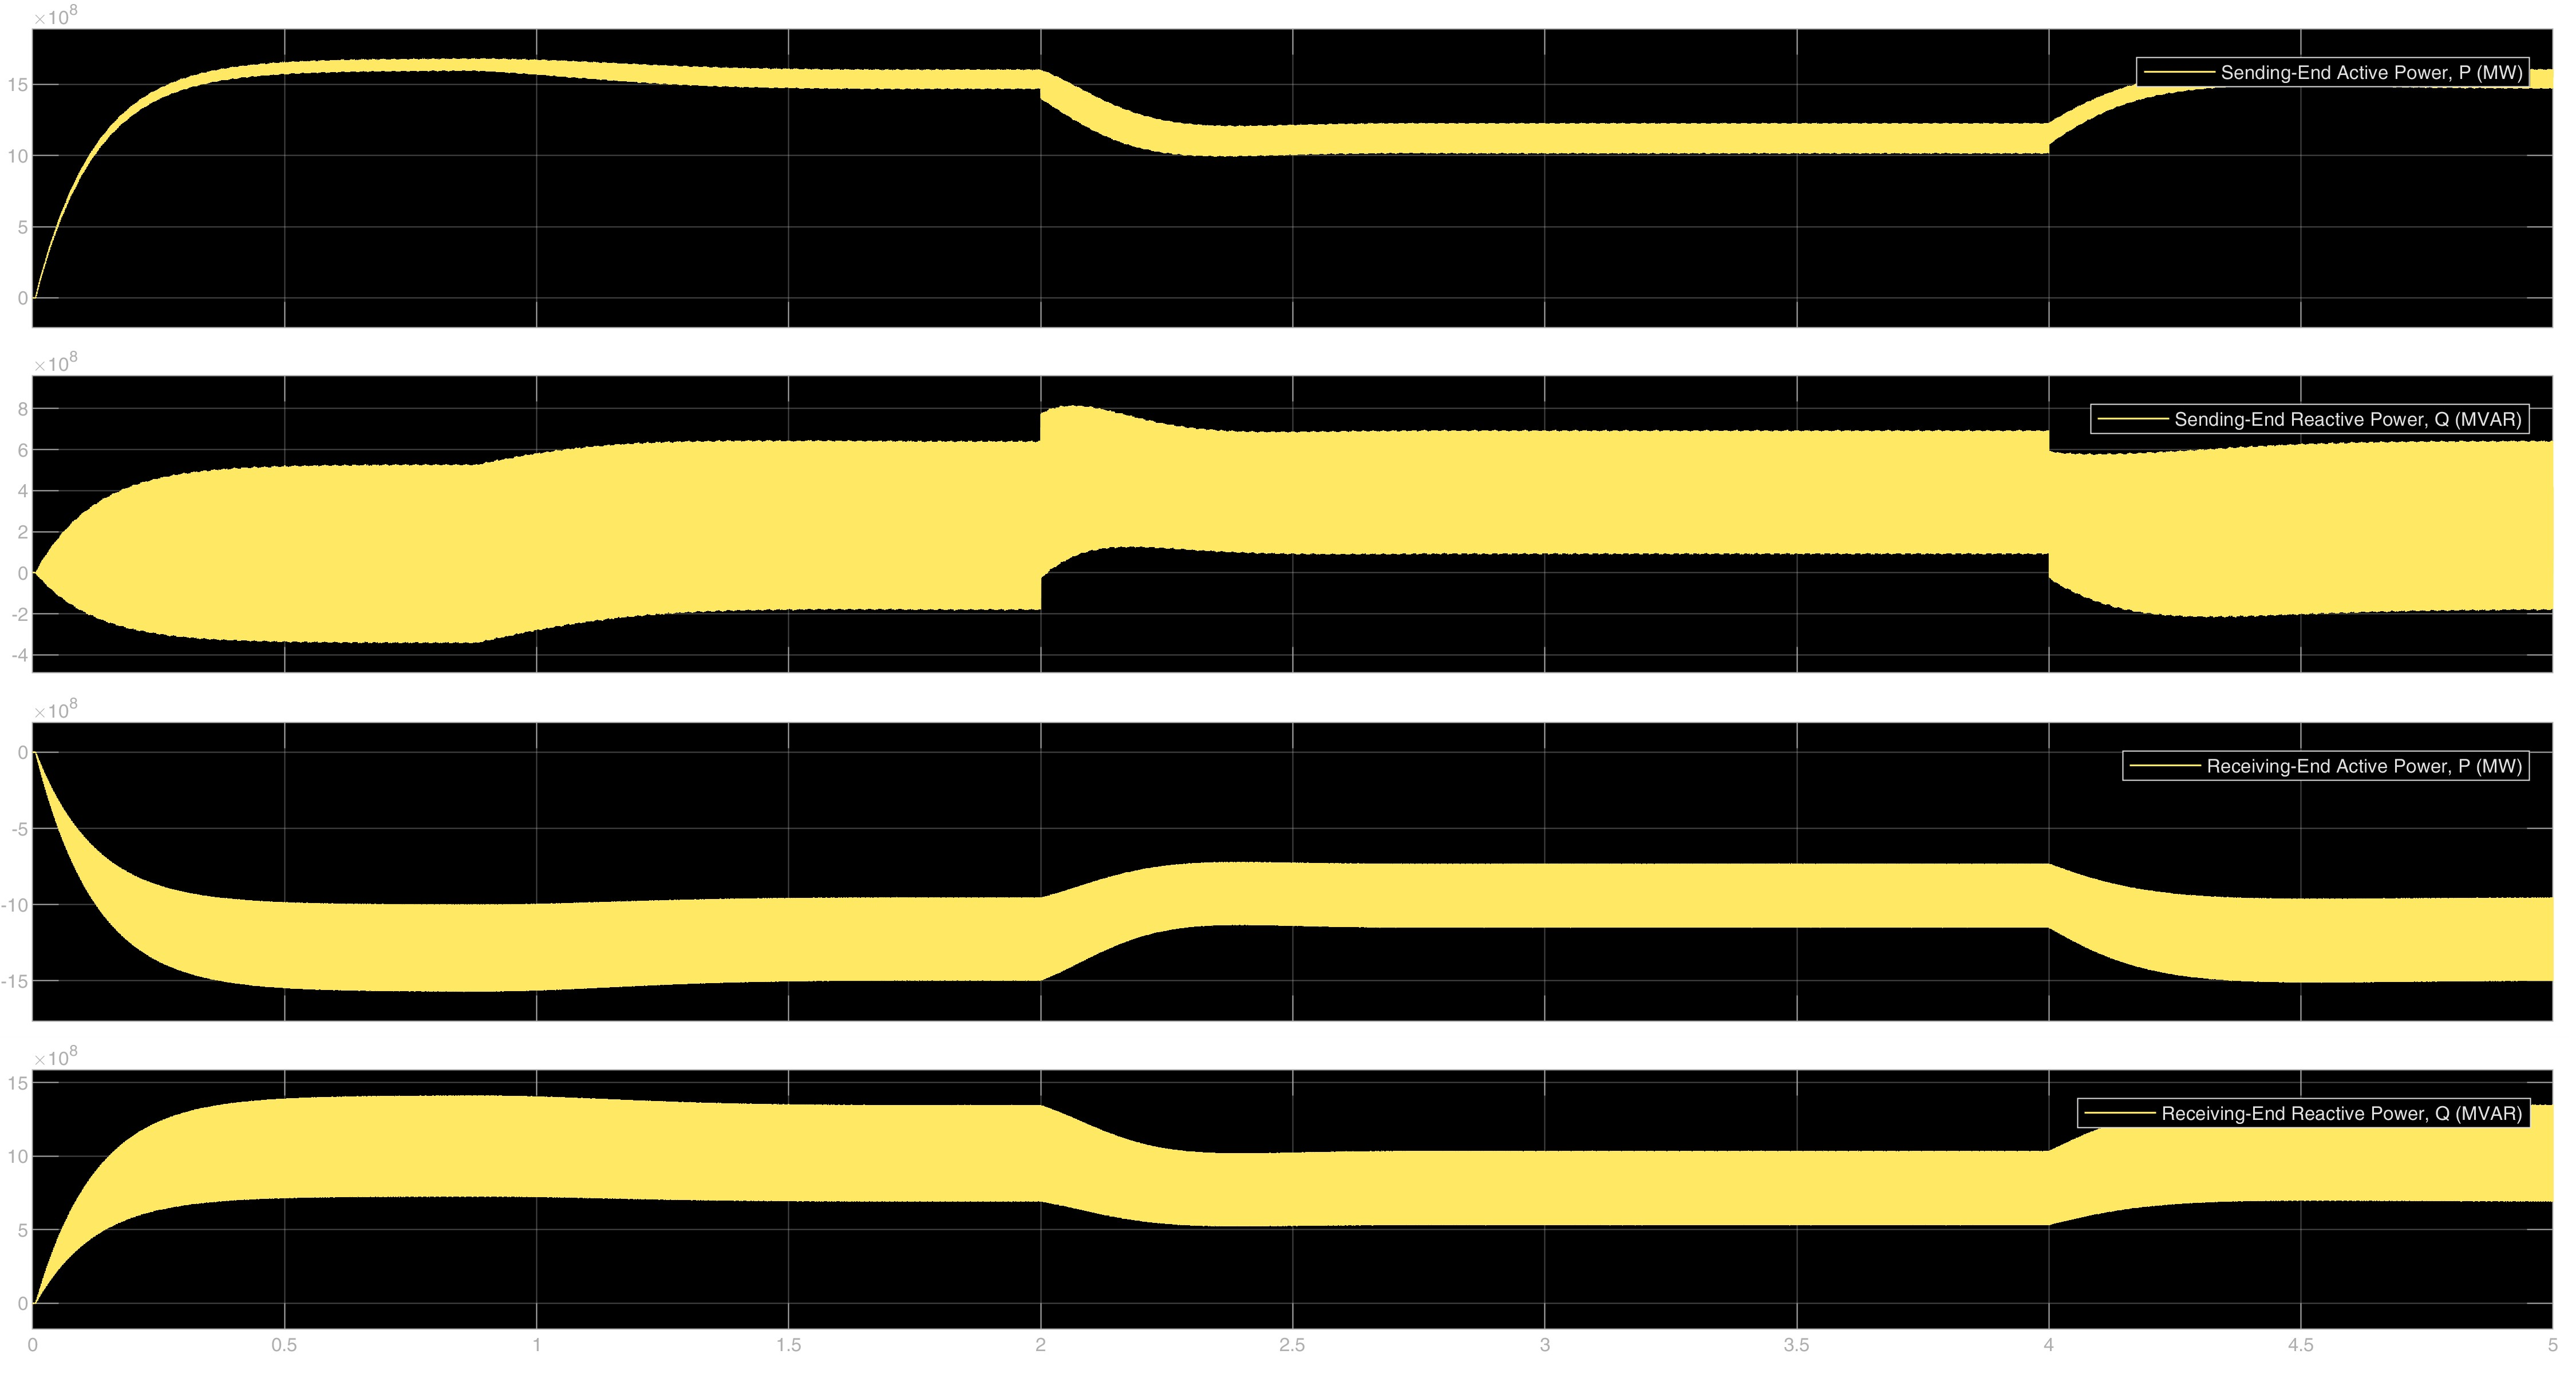
\includegraphics[width=0.95\textwidth]{A_Power.jpg}
    \caption{\textbf{Powers Scope:} Illustrates the corresponding active power ($P$) transmission and reactive power ($Q$) consumption profiles at both ends.}
\end{figure}

\newpage
\subsection{Detailed Waveform Analysis}

\begin{figure}[H]
    \centering
    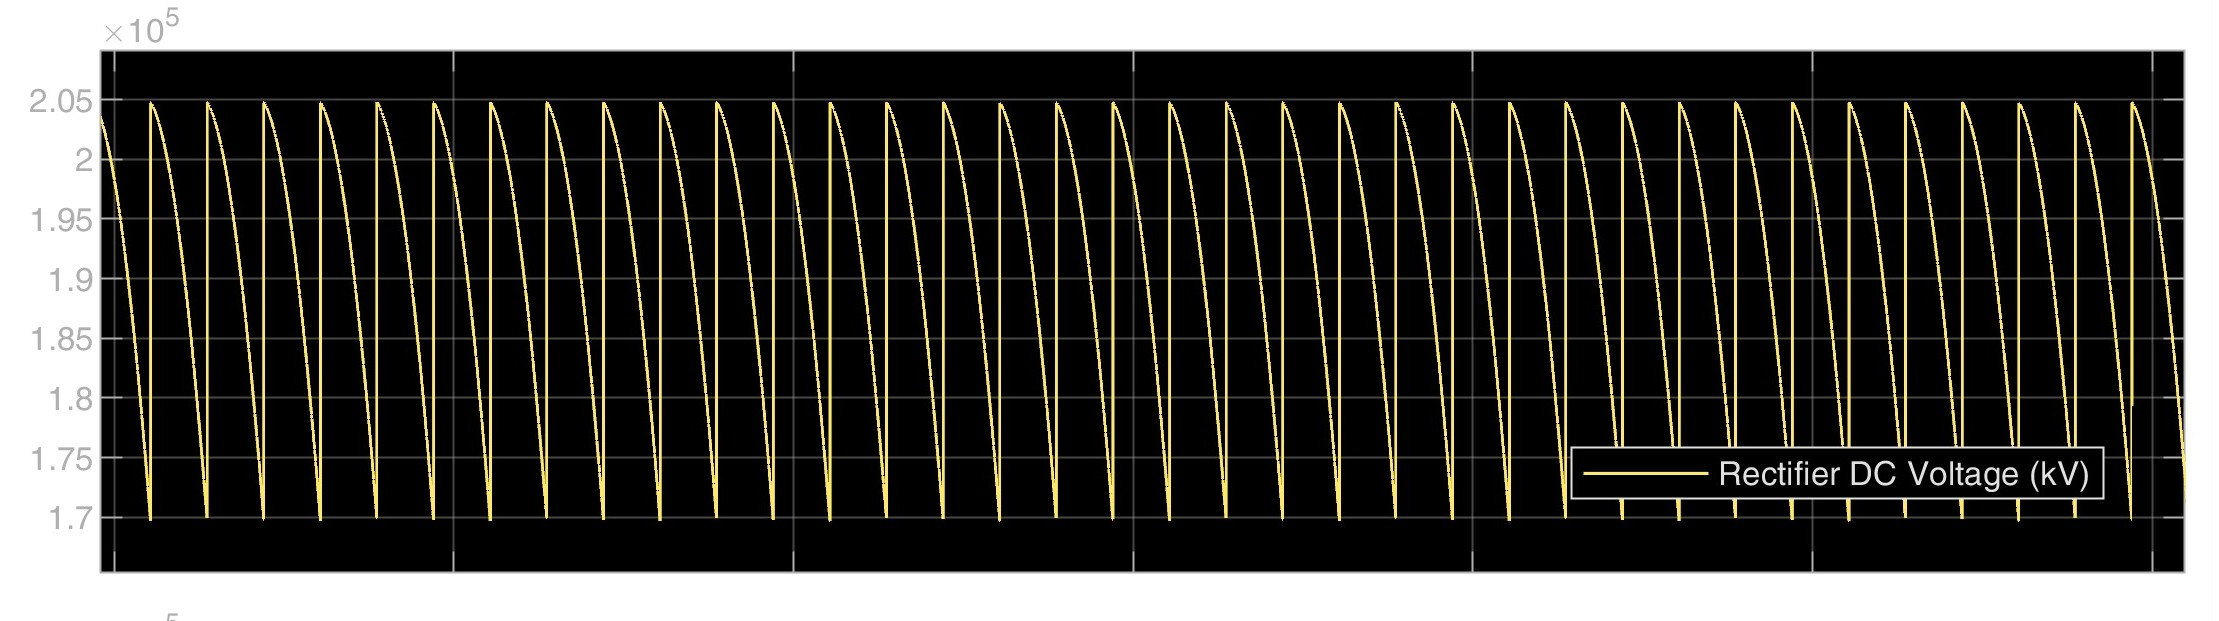
\includegraphics[width=0.75\textwidth]{A_1.jpg}
    \caption{\textbf{Rectifier DC Voltage ($V_{rect}$)}}
\end{figure}
The sending-end DC voltage remains highly stable around the nominal 200 kV mark. The waveform clearly exhibits the characteristic 12-pulse ripples (12 peaks per AC cycle). This 12-pulse configuration is highly efficient, as it significantly reduces the size requirement for the DC smoothing reactor while providing a high-quality DC output.

\vspace{0.5cm}
\begin{figure}[H]
    \centering
    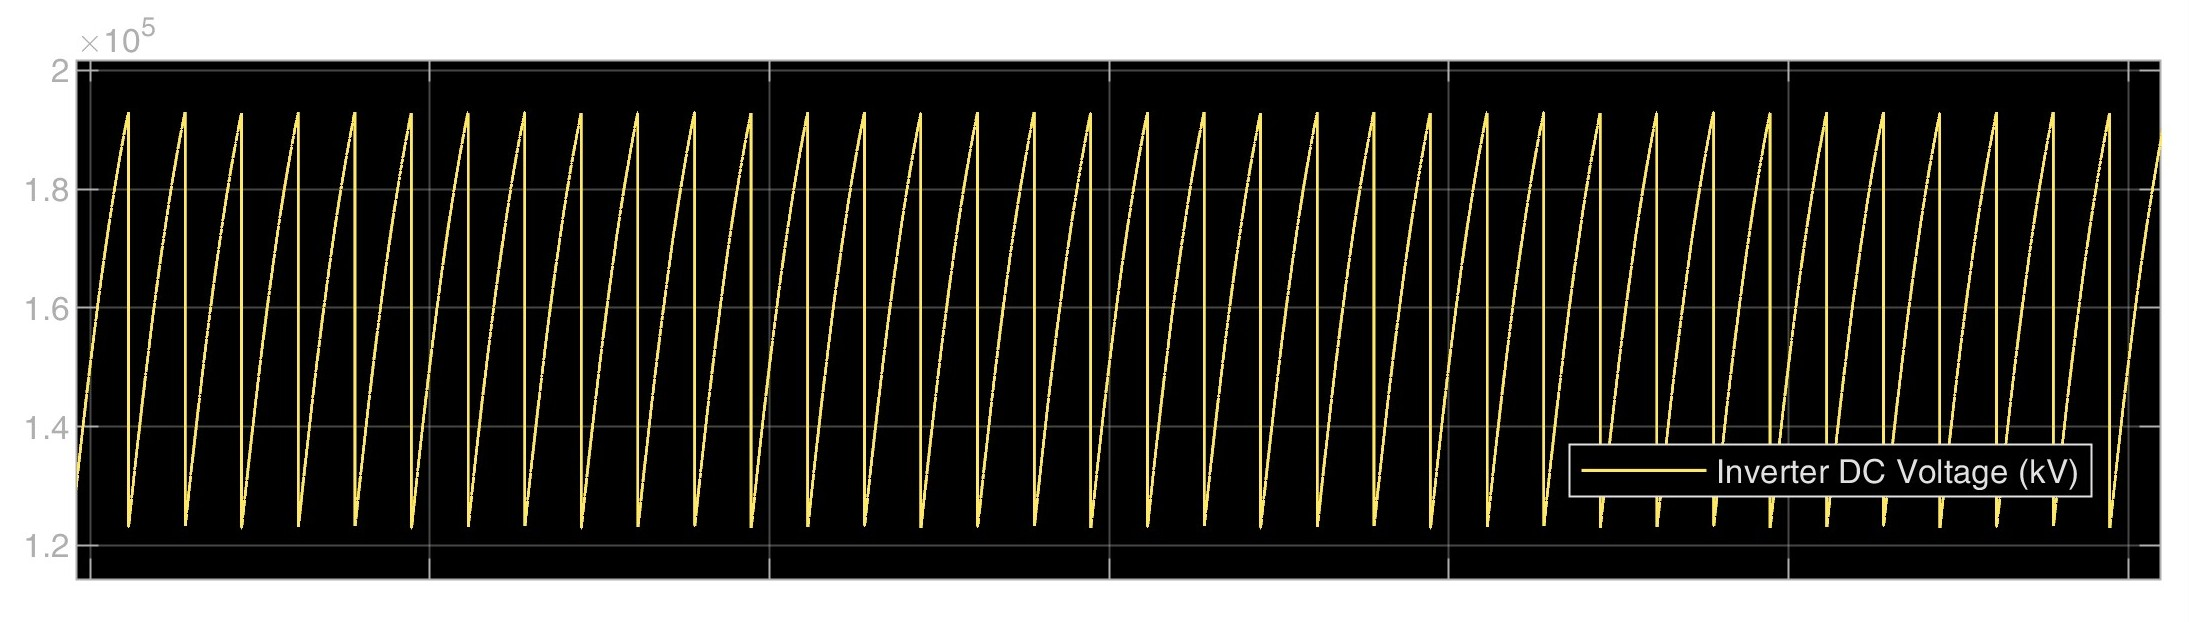
\includegraphics[width=0.75\textwidth]{A_2.jpg}
    \caption{\textbf{Inverter DC Voltage ($V_{inv}$)}}
\end{figure}
The receiving-end DC voltage acts as a controlled back-EMF. Operating in the inversion region ($\alpha > 90^{\circ}$), it maintains a negative average voltage. The potential difference ($\Delta V$) between the rectifier and the inverter is the driving force that pushes the DC link current across the transmission line resistance.

\vspace{0.5cm}
\begin{figure}[H]
    \centering
    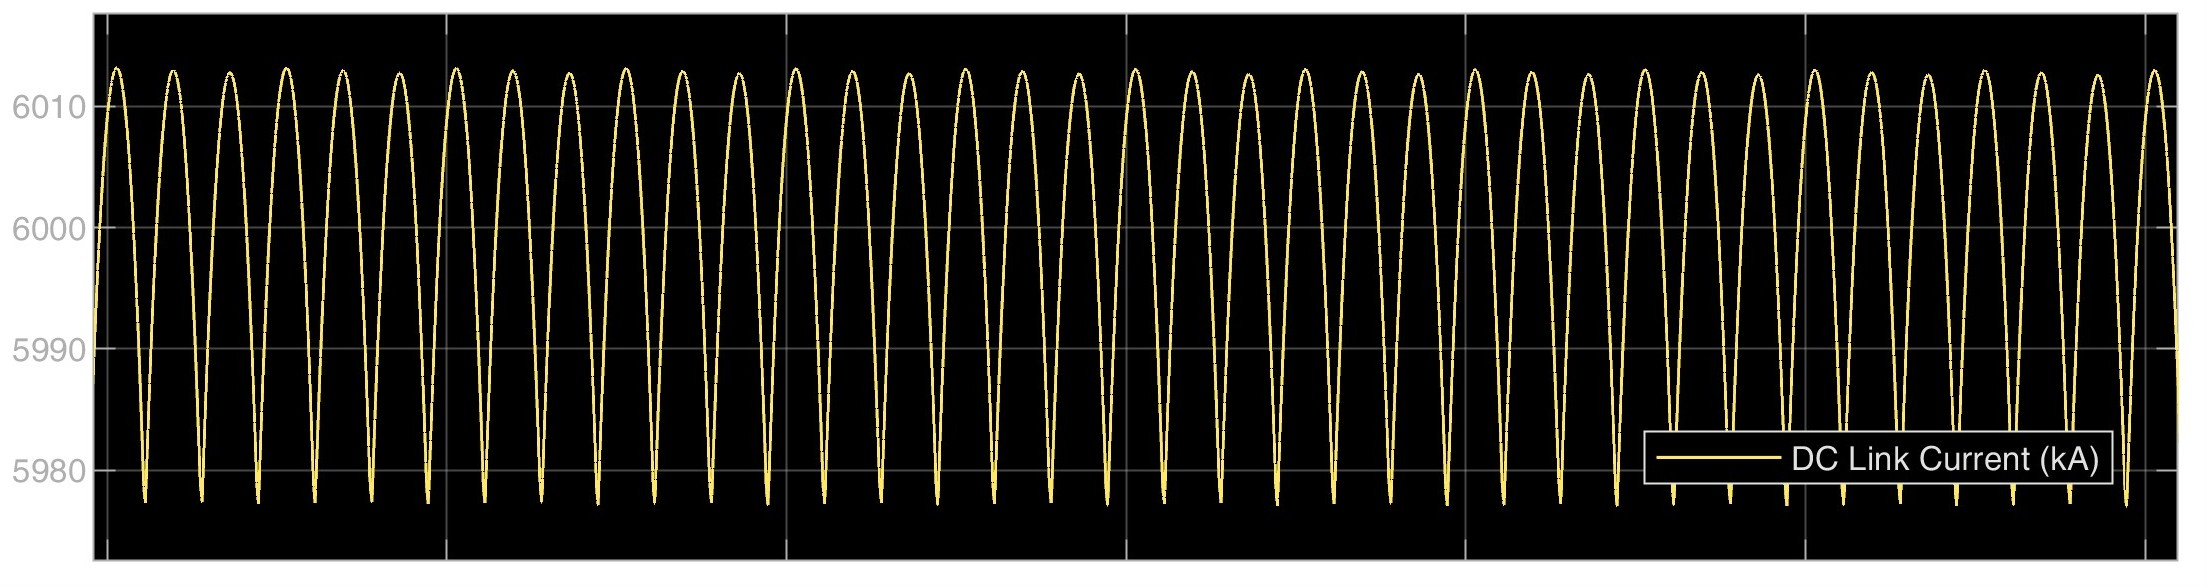
\includegraphics[width=0.75\textwidth]{A_3.jpg}
    \caption{\textbf{DC Link Current ($I_{dc}$)}}
\end{figure}
The DC current perfectly mirrors the applied reference signal. Upon the application of step changes (e.g., at $t=2s$ and $t=4s$), the current transitions smoothly with an extremely fast settling time, zero steady-state error, and negligible overshoot. This confirms the optimal tuning of the rectifier's PI current controller.

\vspace{0.5cm}
\begin{figure}[H]
    \centering
    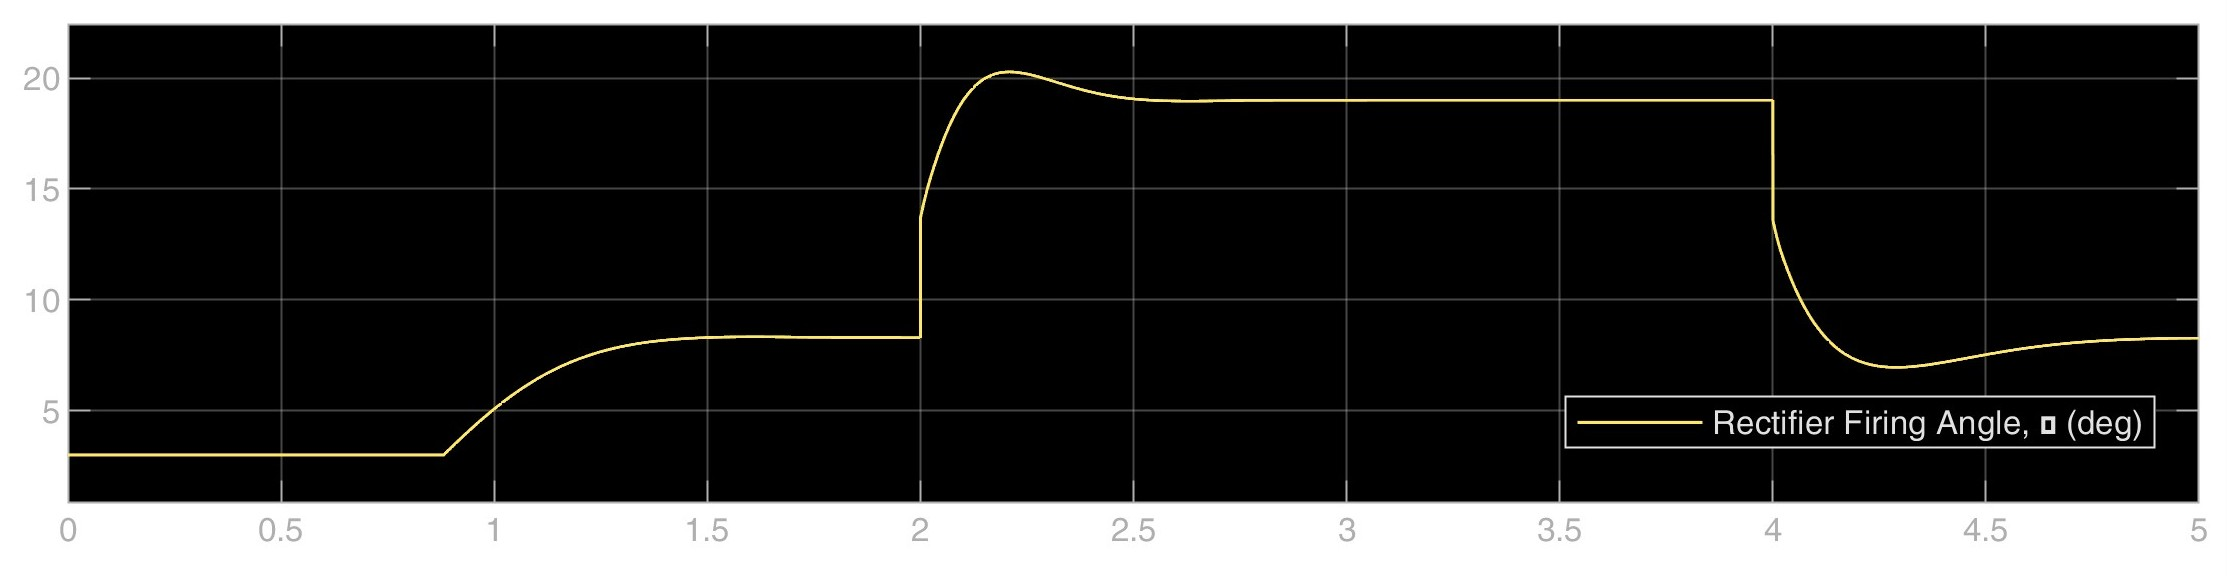
\includegraphics[width=0.75\textwidth]{A_4.jpg}
    \caption{\textbf{Rectifier Firing Angle ($\alpha_{rect}$)}}
\end{figure}
The rectifier firing angle dynamically modulates within the active rectification zone (typically $10^{\circ}$ to $30^{\circ}$ during steady state) to strictly regulate the DC current. When a lower current is demanded, the PI controller seamlessly increases the firing angle to lower the output voltage, thereby reducing the line current.

\vspace{0.5cm}
\begin{figure}[H]
    \centering
    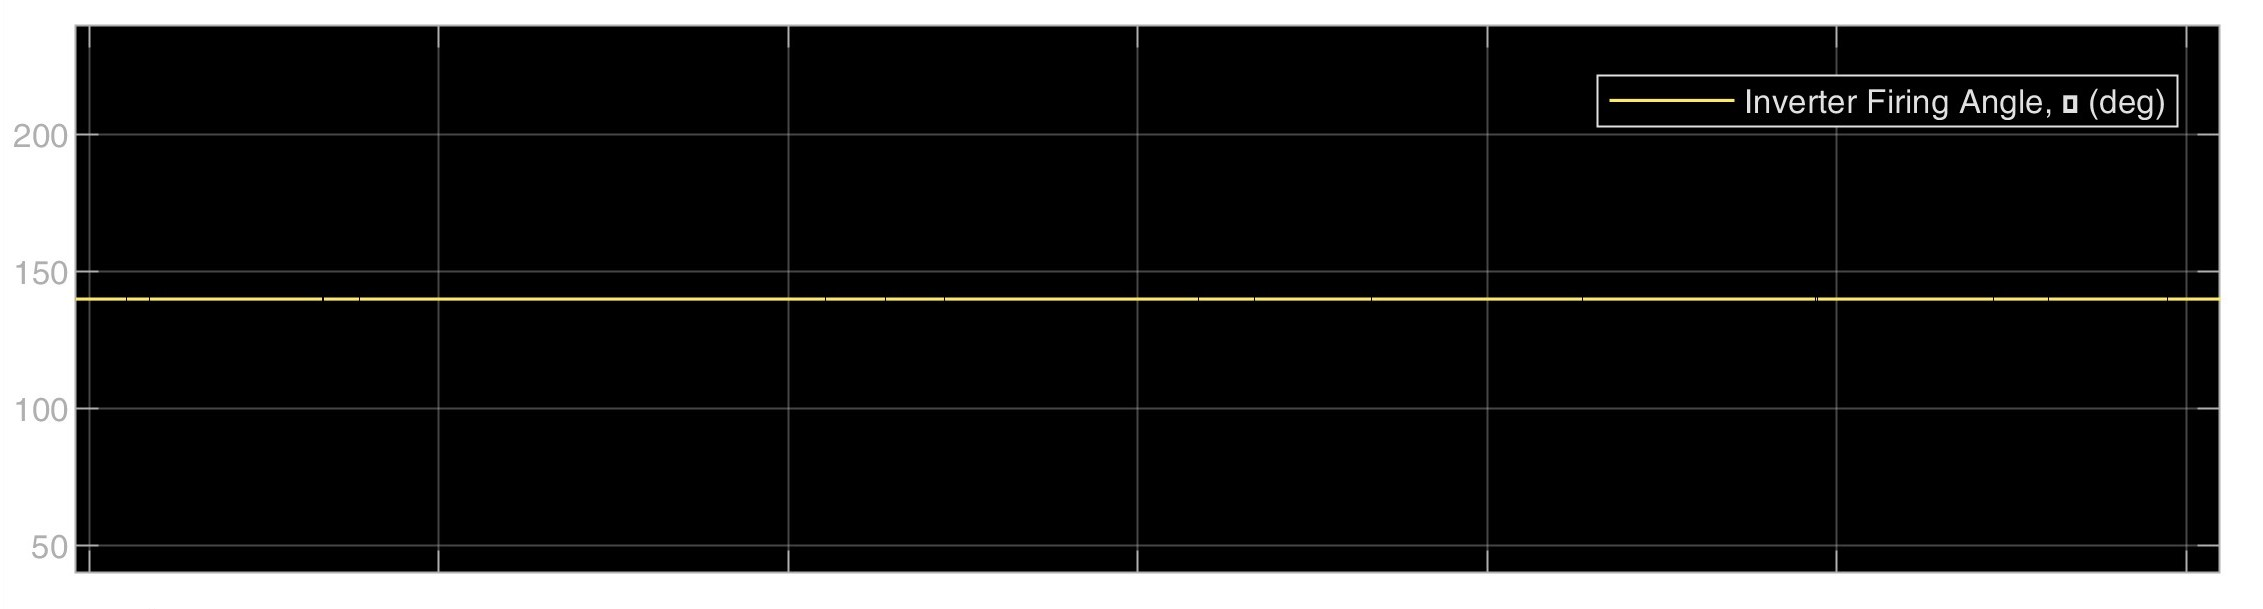
\includegraphics[width=0.75\textwidth]{A_5.jpg}
    \caption{\textbf{Inverter Firing Angle ($\gamma_{inv}$)}}
\end{figure}
The inverter operates under Constant Extinction Angle (CEA) control, firmly maintaining $\gamma$ at $40^{\circ}$. This fixed margin ensures that the thyristors have sufficient time to regain their forward-blocking capability before the voltage polarity reverses, effectively protecting the inverter against catastrophic commutation failures.

\vspace{0.5cm}
\begin{figure}[H]
    \centering
    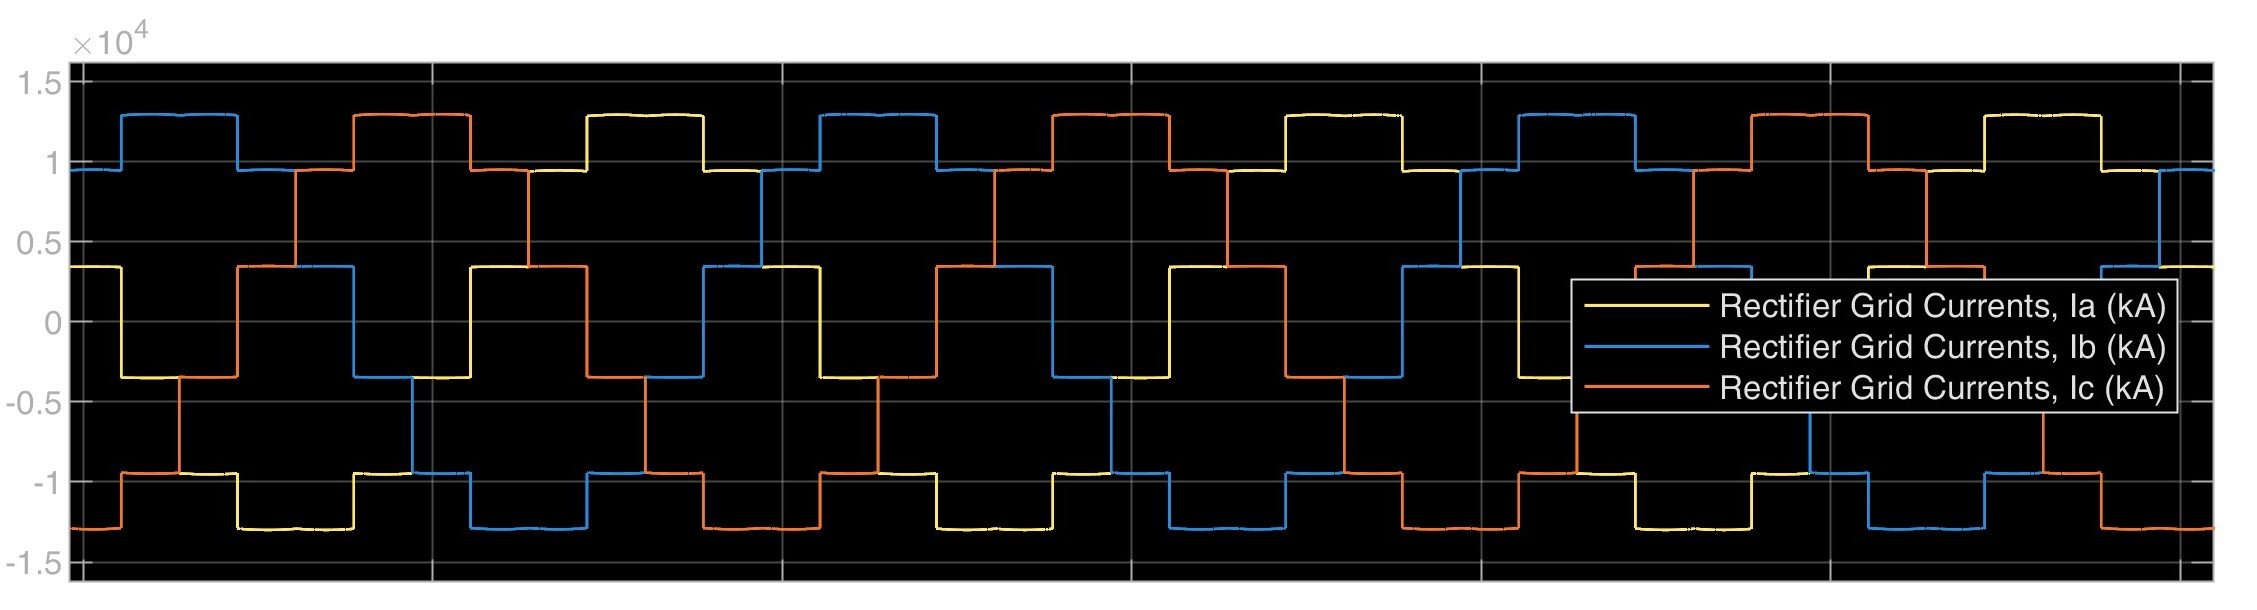
\includegraphics[width=0.75\textwidth]{A_6.jpg}
    \caption{\textbf{Rectifier AC Grid Currents}}
\end{figure}
The three-phase AC currents drawn from the sending-end grid exhibit a balanced quasi-square waveform. The implementation of the $Y-Y$ and $Y-\Delta$ transformer arrangements inherently cancels out the 5th and 7th harmonics, resulting in a cleaner 12-step waveform that approximates a sinusoidal shape, reducing filtering requirements.

\vspace{0.5cm}
\begin{figure}[H]
    \centering
    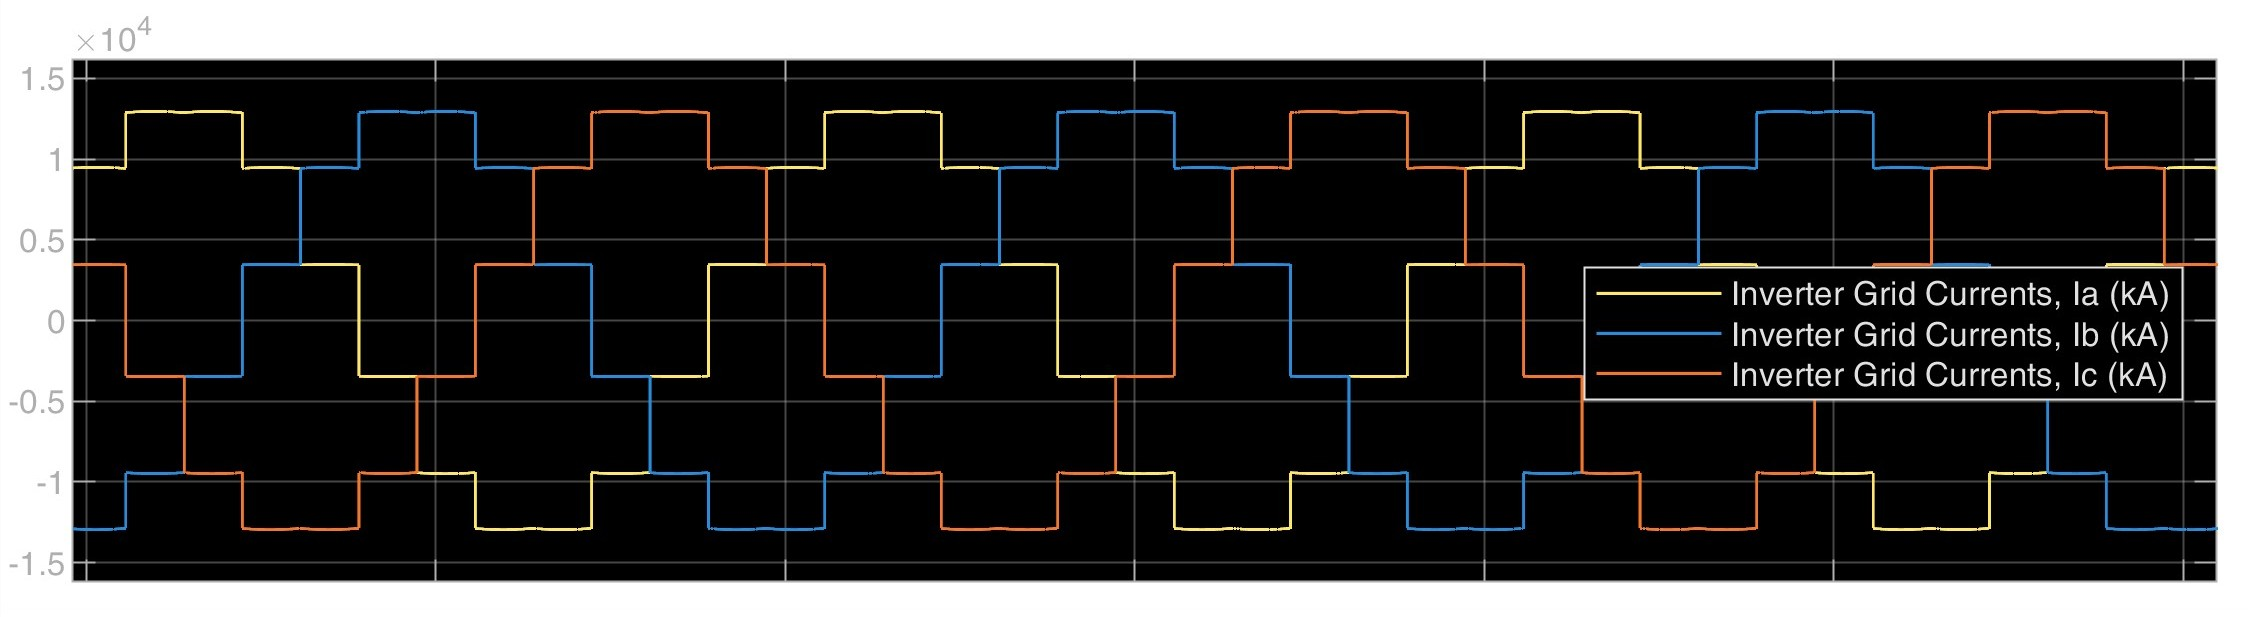
\includegraphics[width=0.75\textwidth]{A_7.jpg}
    \caption{\textbf{Inverter AC Grid Currents}}
\end{figure}
Similar to the rectifier, the AC currents injected into the receiving grid are balanced and low in harmonic distortion. The amplitude of these currents is directly proportional to the active power being delivered to the receiving network.

\vspace{0.5cm}
\begin{figure}[H]
    \centering
    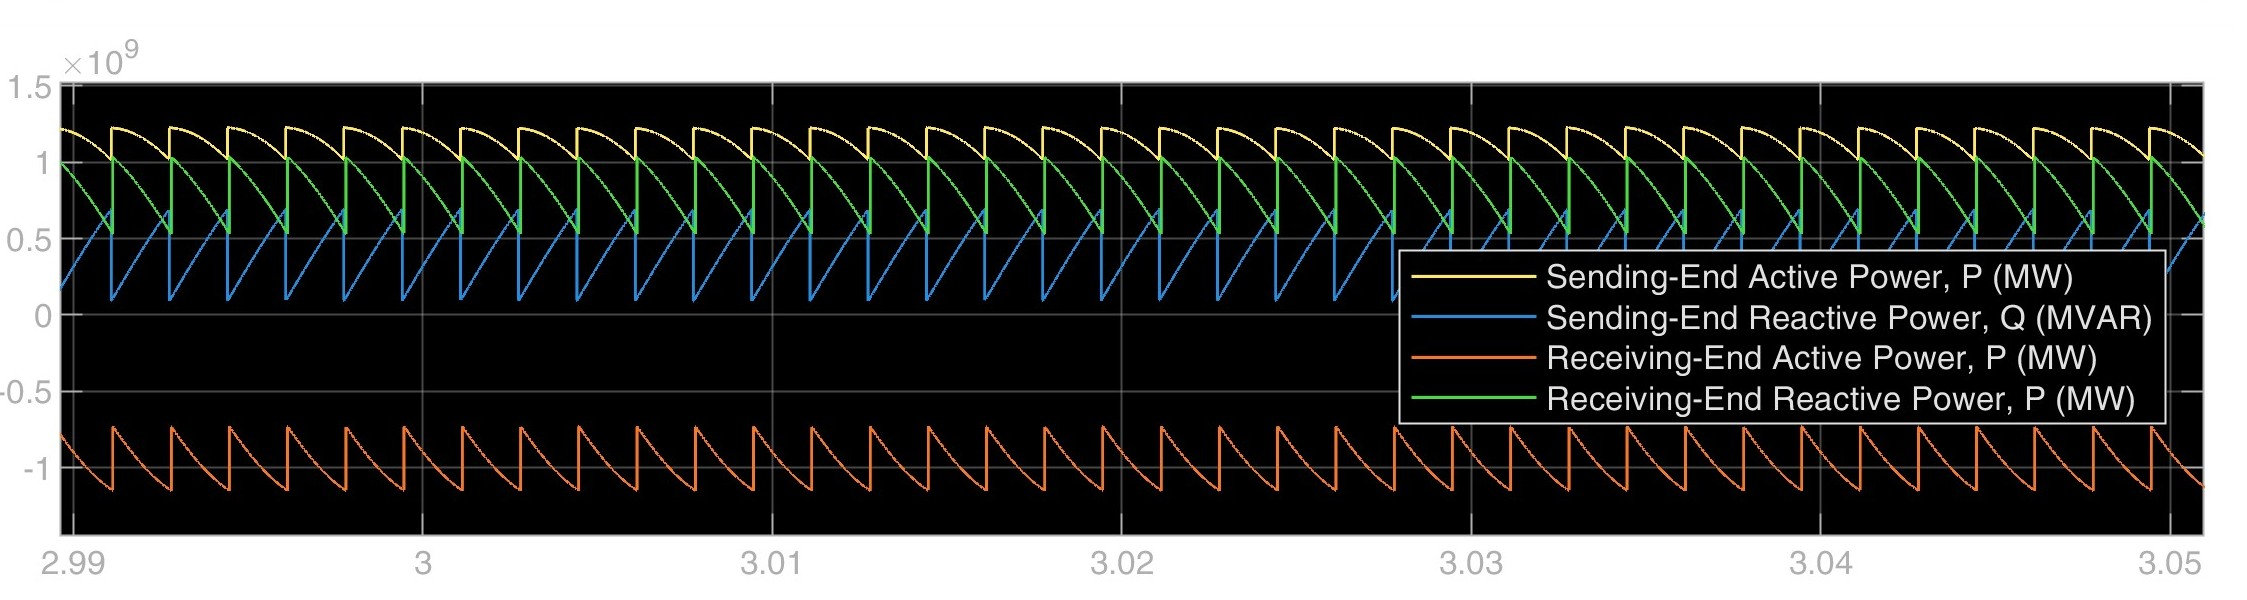
\includegraphics[width=0.75\textwidth]{A_8.jpg}
    \caption{\textbf{Active and Reactive Power ($P \& Q$)}}
\end{figure}
The active power ($P$) accurately tracks the step changes of the DC current, proving efficient energy transfer. Meanwhile, Line-Commutated Converters (LCCs) inevitably consume reactive power ($Q$). The reactive power demand is clearly visible and fluctuates directly with the firing angles; larger firing angles result in higher reactive power consumption from the AC grid.

\newpage

% ========================================================= %
% ----------------------- CASE B -------------------------- %
% ========================================================= %
\section{Case B: Severe Sag Condition}
This case investigates the system's dynamic resilience and control adaptability during a severe 25\% voltage sag occurring at the rectifier's AC grid. When the sending-end AC voltage drops significantly, the rectifier struggles to generate sufficient DC voltage to drive the commanded DC current across the transmission line. In an attempt to compensate, the rectifier's PI controller aggressively decreases the firing angle until it hits the absolute hardware lower limit ($\alpha_{min} = 3^{\circ}$). 

At this saturation point, the rectifier falls into Constant Ignition Angle (CIA) mode and entirely loses its ability to regulate the current. To prevent the DC link current from collapsing to zero, a contingency control strategy dictates that the Inverter must seamlessly take over the Constant Current (CC) regulation. This operational transition is achieved by subtracting a 5\% Current Margin from the original current reference, ensuring that the inverter's CC controller becomes active and assumes total control of the power flow to sustain grid stability.

\subsection{System Configuration (Case B Modifications)}
Figure 12 details the system configuration after implementing the necessary modifications to facilitate the current control handover for Case B. A \texttt{Goto} global tag (labeled \texttt{IDC}) was attached to the sending-end DC current measurement block. This signal is wirelessly routed to a corresponding \texttt{From} tag inside the receiving-end control subsystem, allowing the inverter to modulate its firing angle dynamically and effectively replace the rectifier as the primary current regulator.

\begin{figure}[H]
    \centering
    \begin{subfigure}{0.48\textwidth}
        \centering
        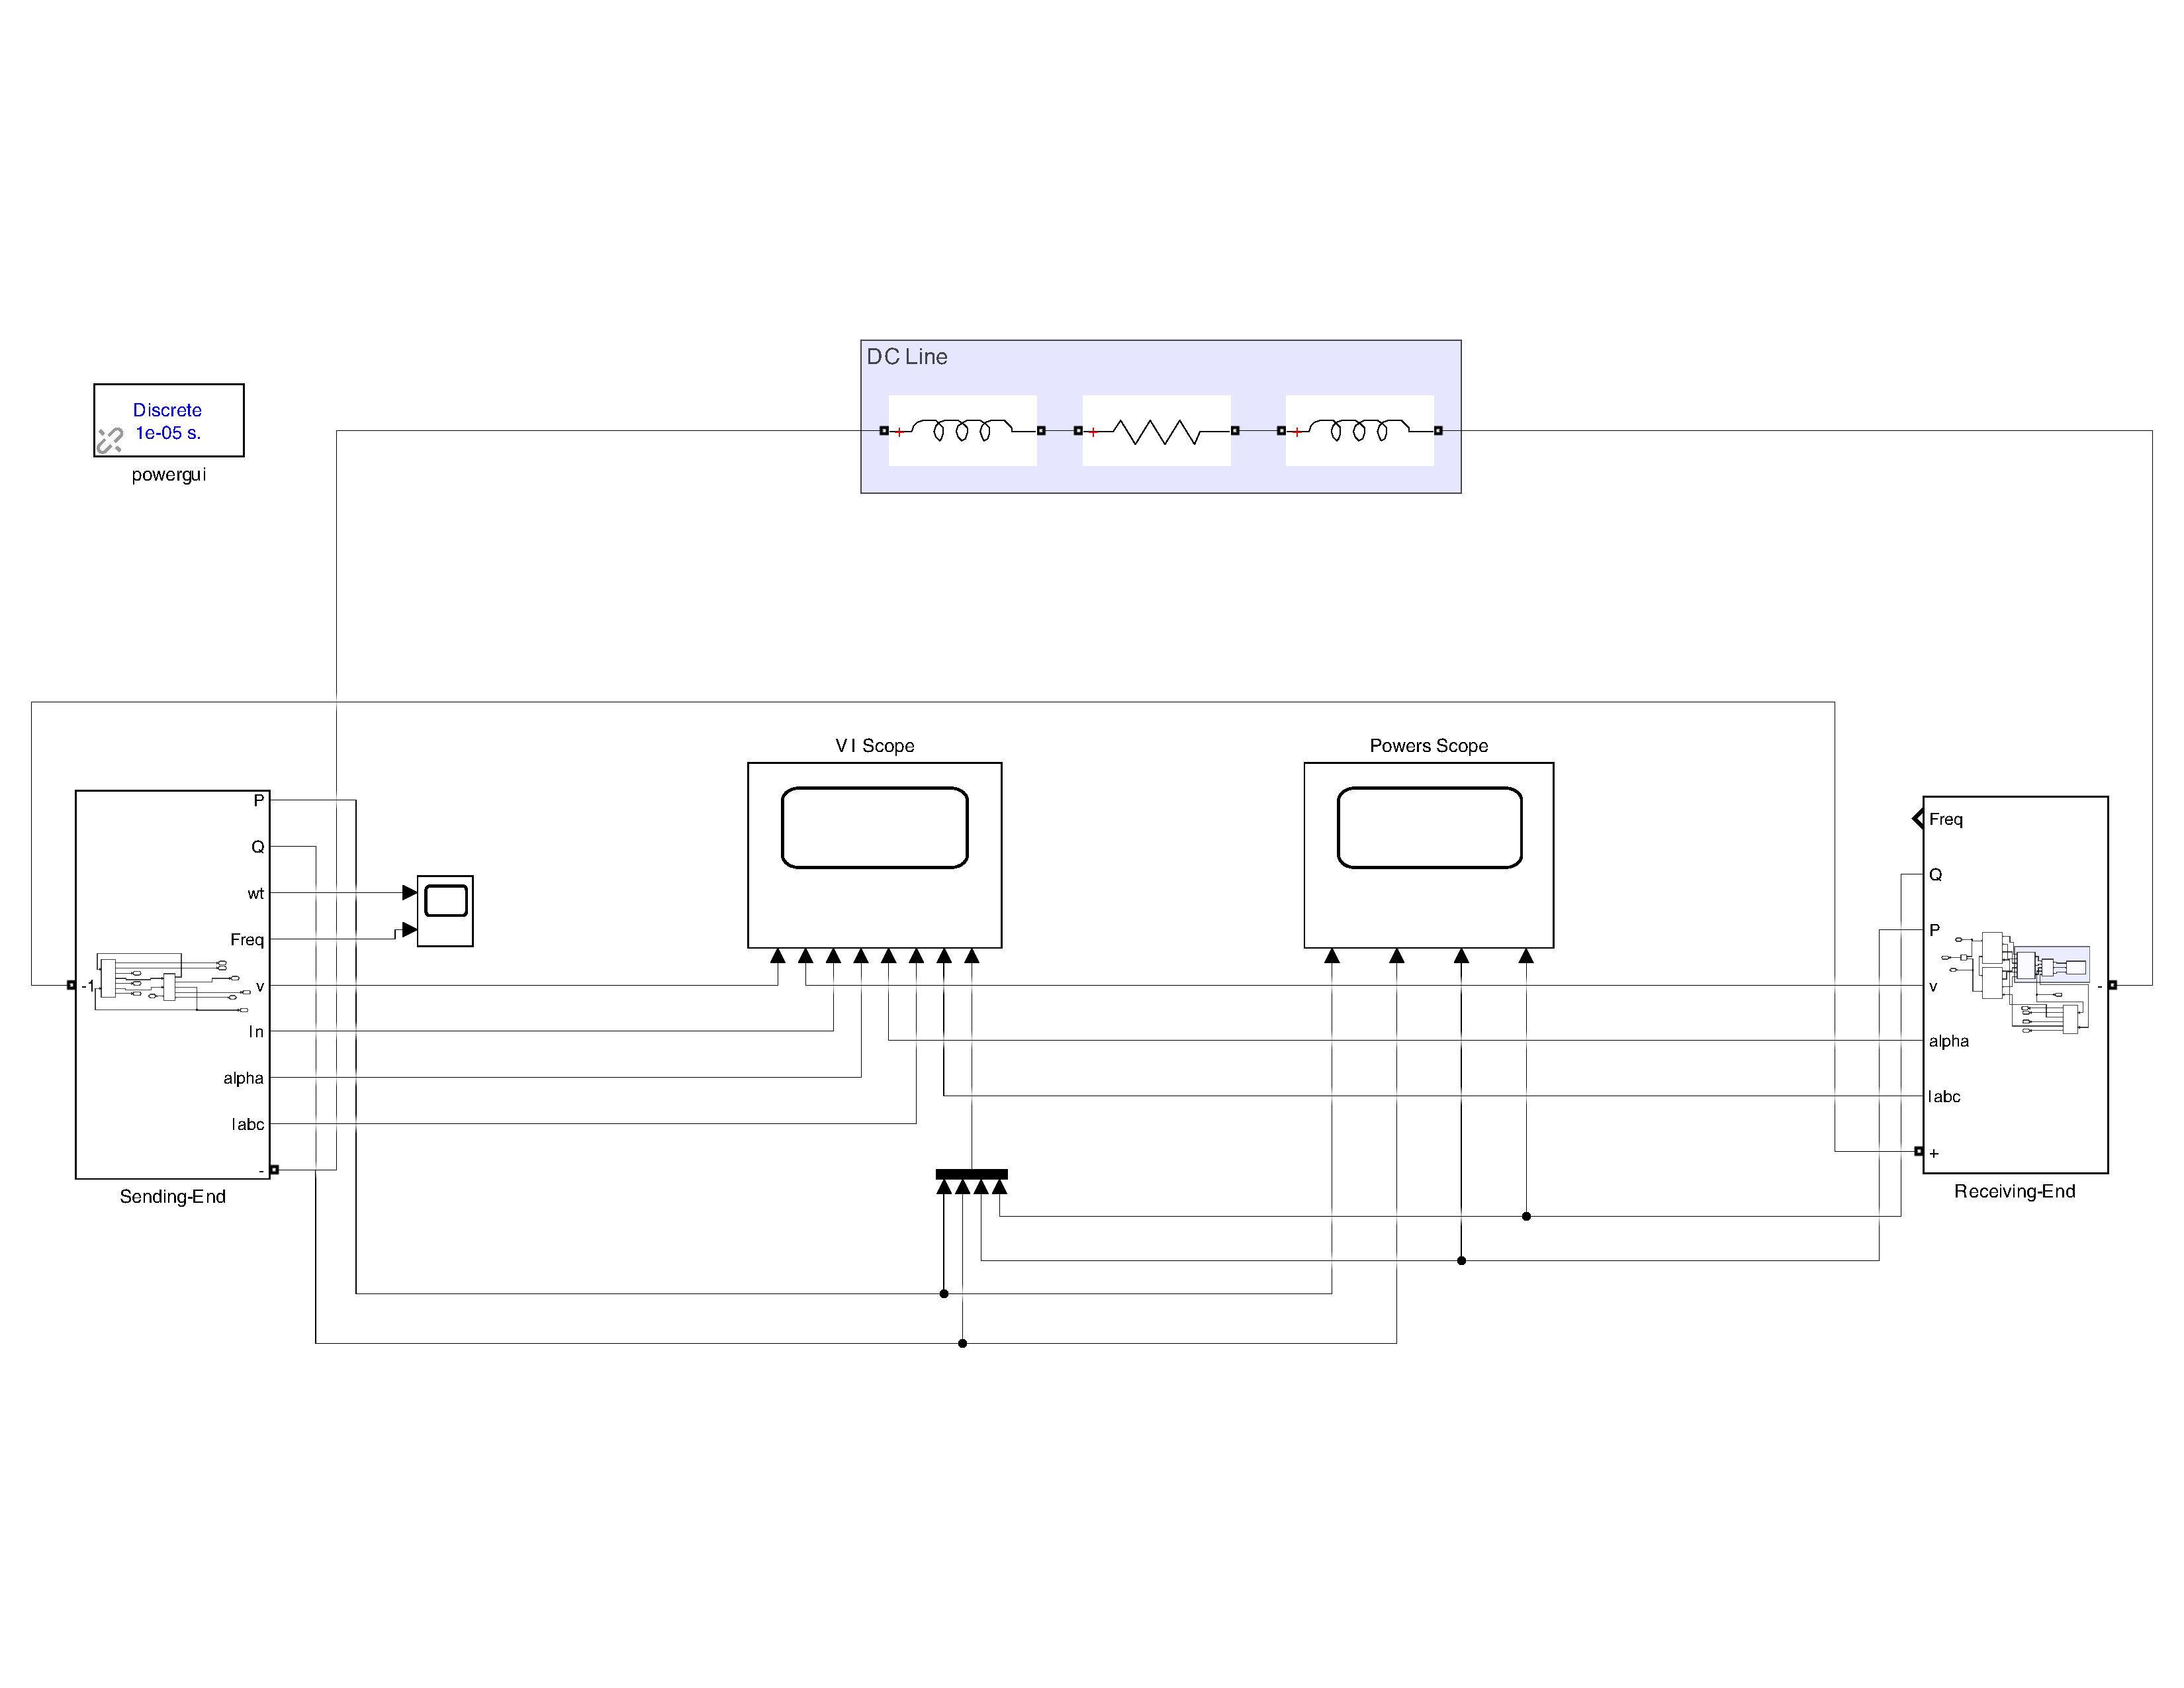
\includegraphics[width=\textwidth]{B_sys1.jpg}
        \caption{\textbf{Main System:}}
    \end{subfigure}
    \hfill
    \begin{subfigure}{0.48\textwidth}
        \centering
        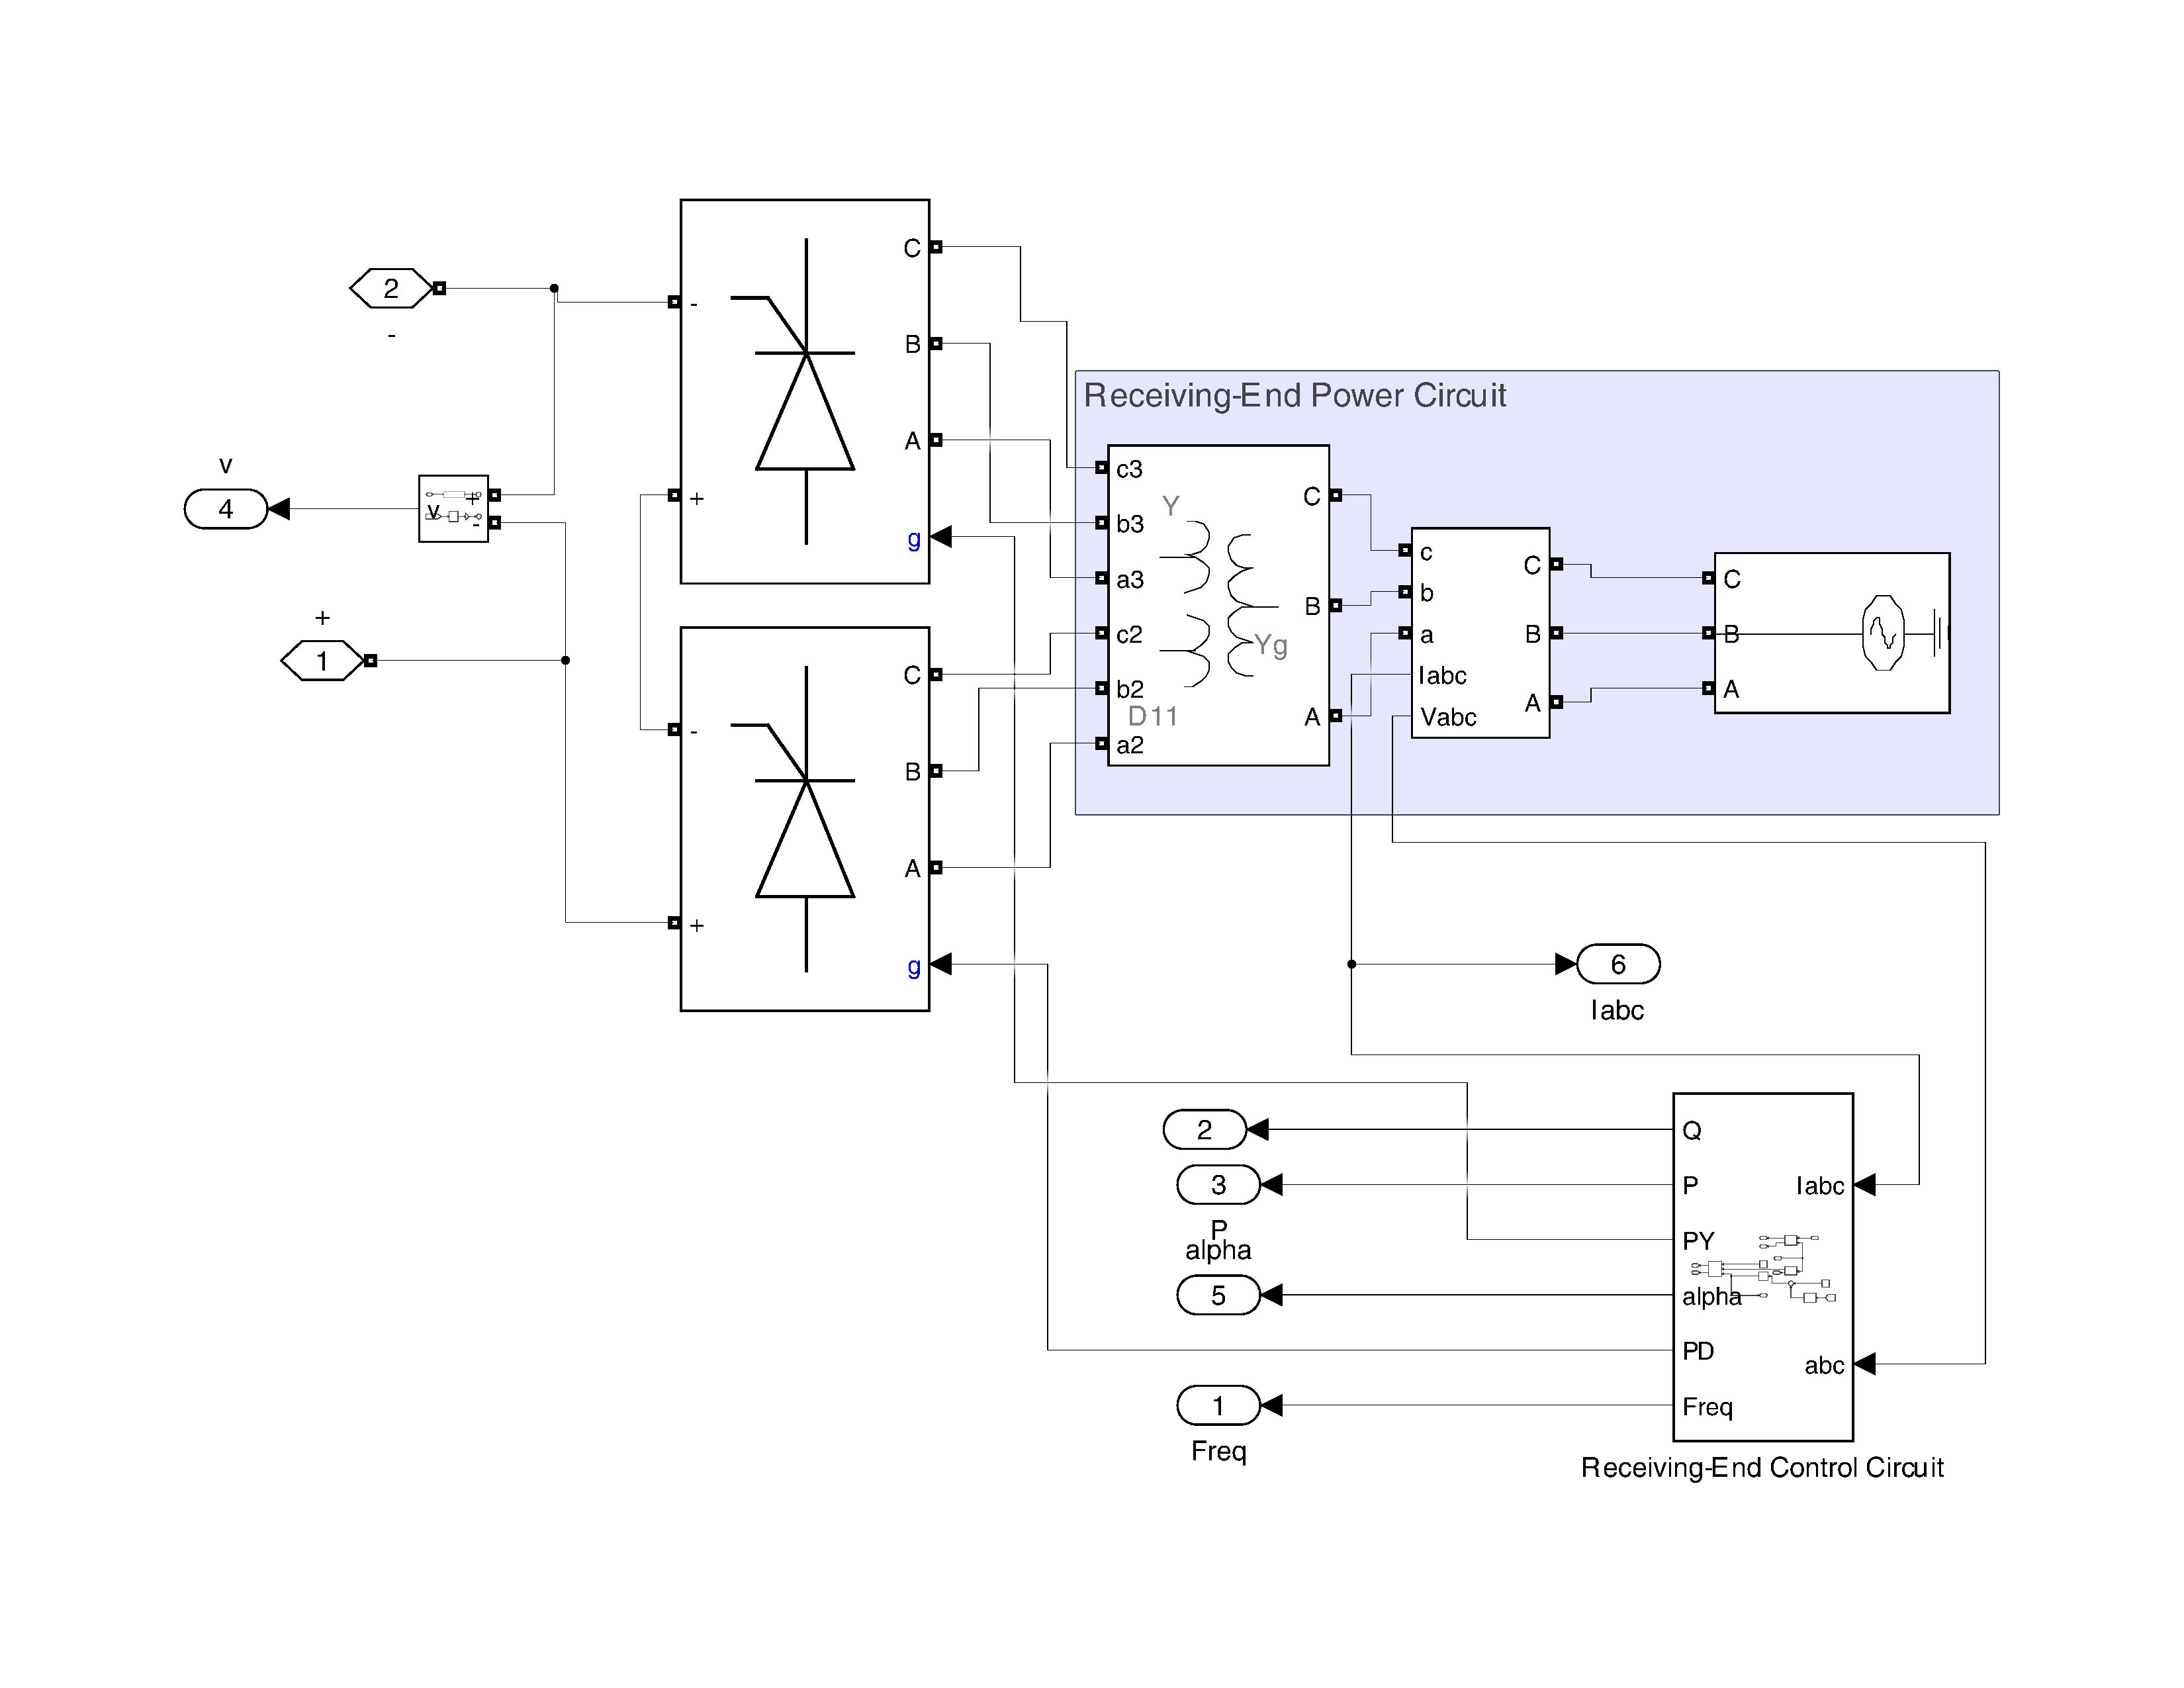
\includegraphics[width=\textwidth]{B_sys2.jpg}
        \caption{\textbf{Receiving Power Circuit:}}
    \end{subfigure}
    
    \vspace{0.3cm}
    \begin{subfigure}{0.48\textwidth}
        \centering
        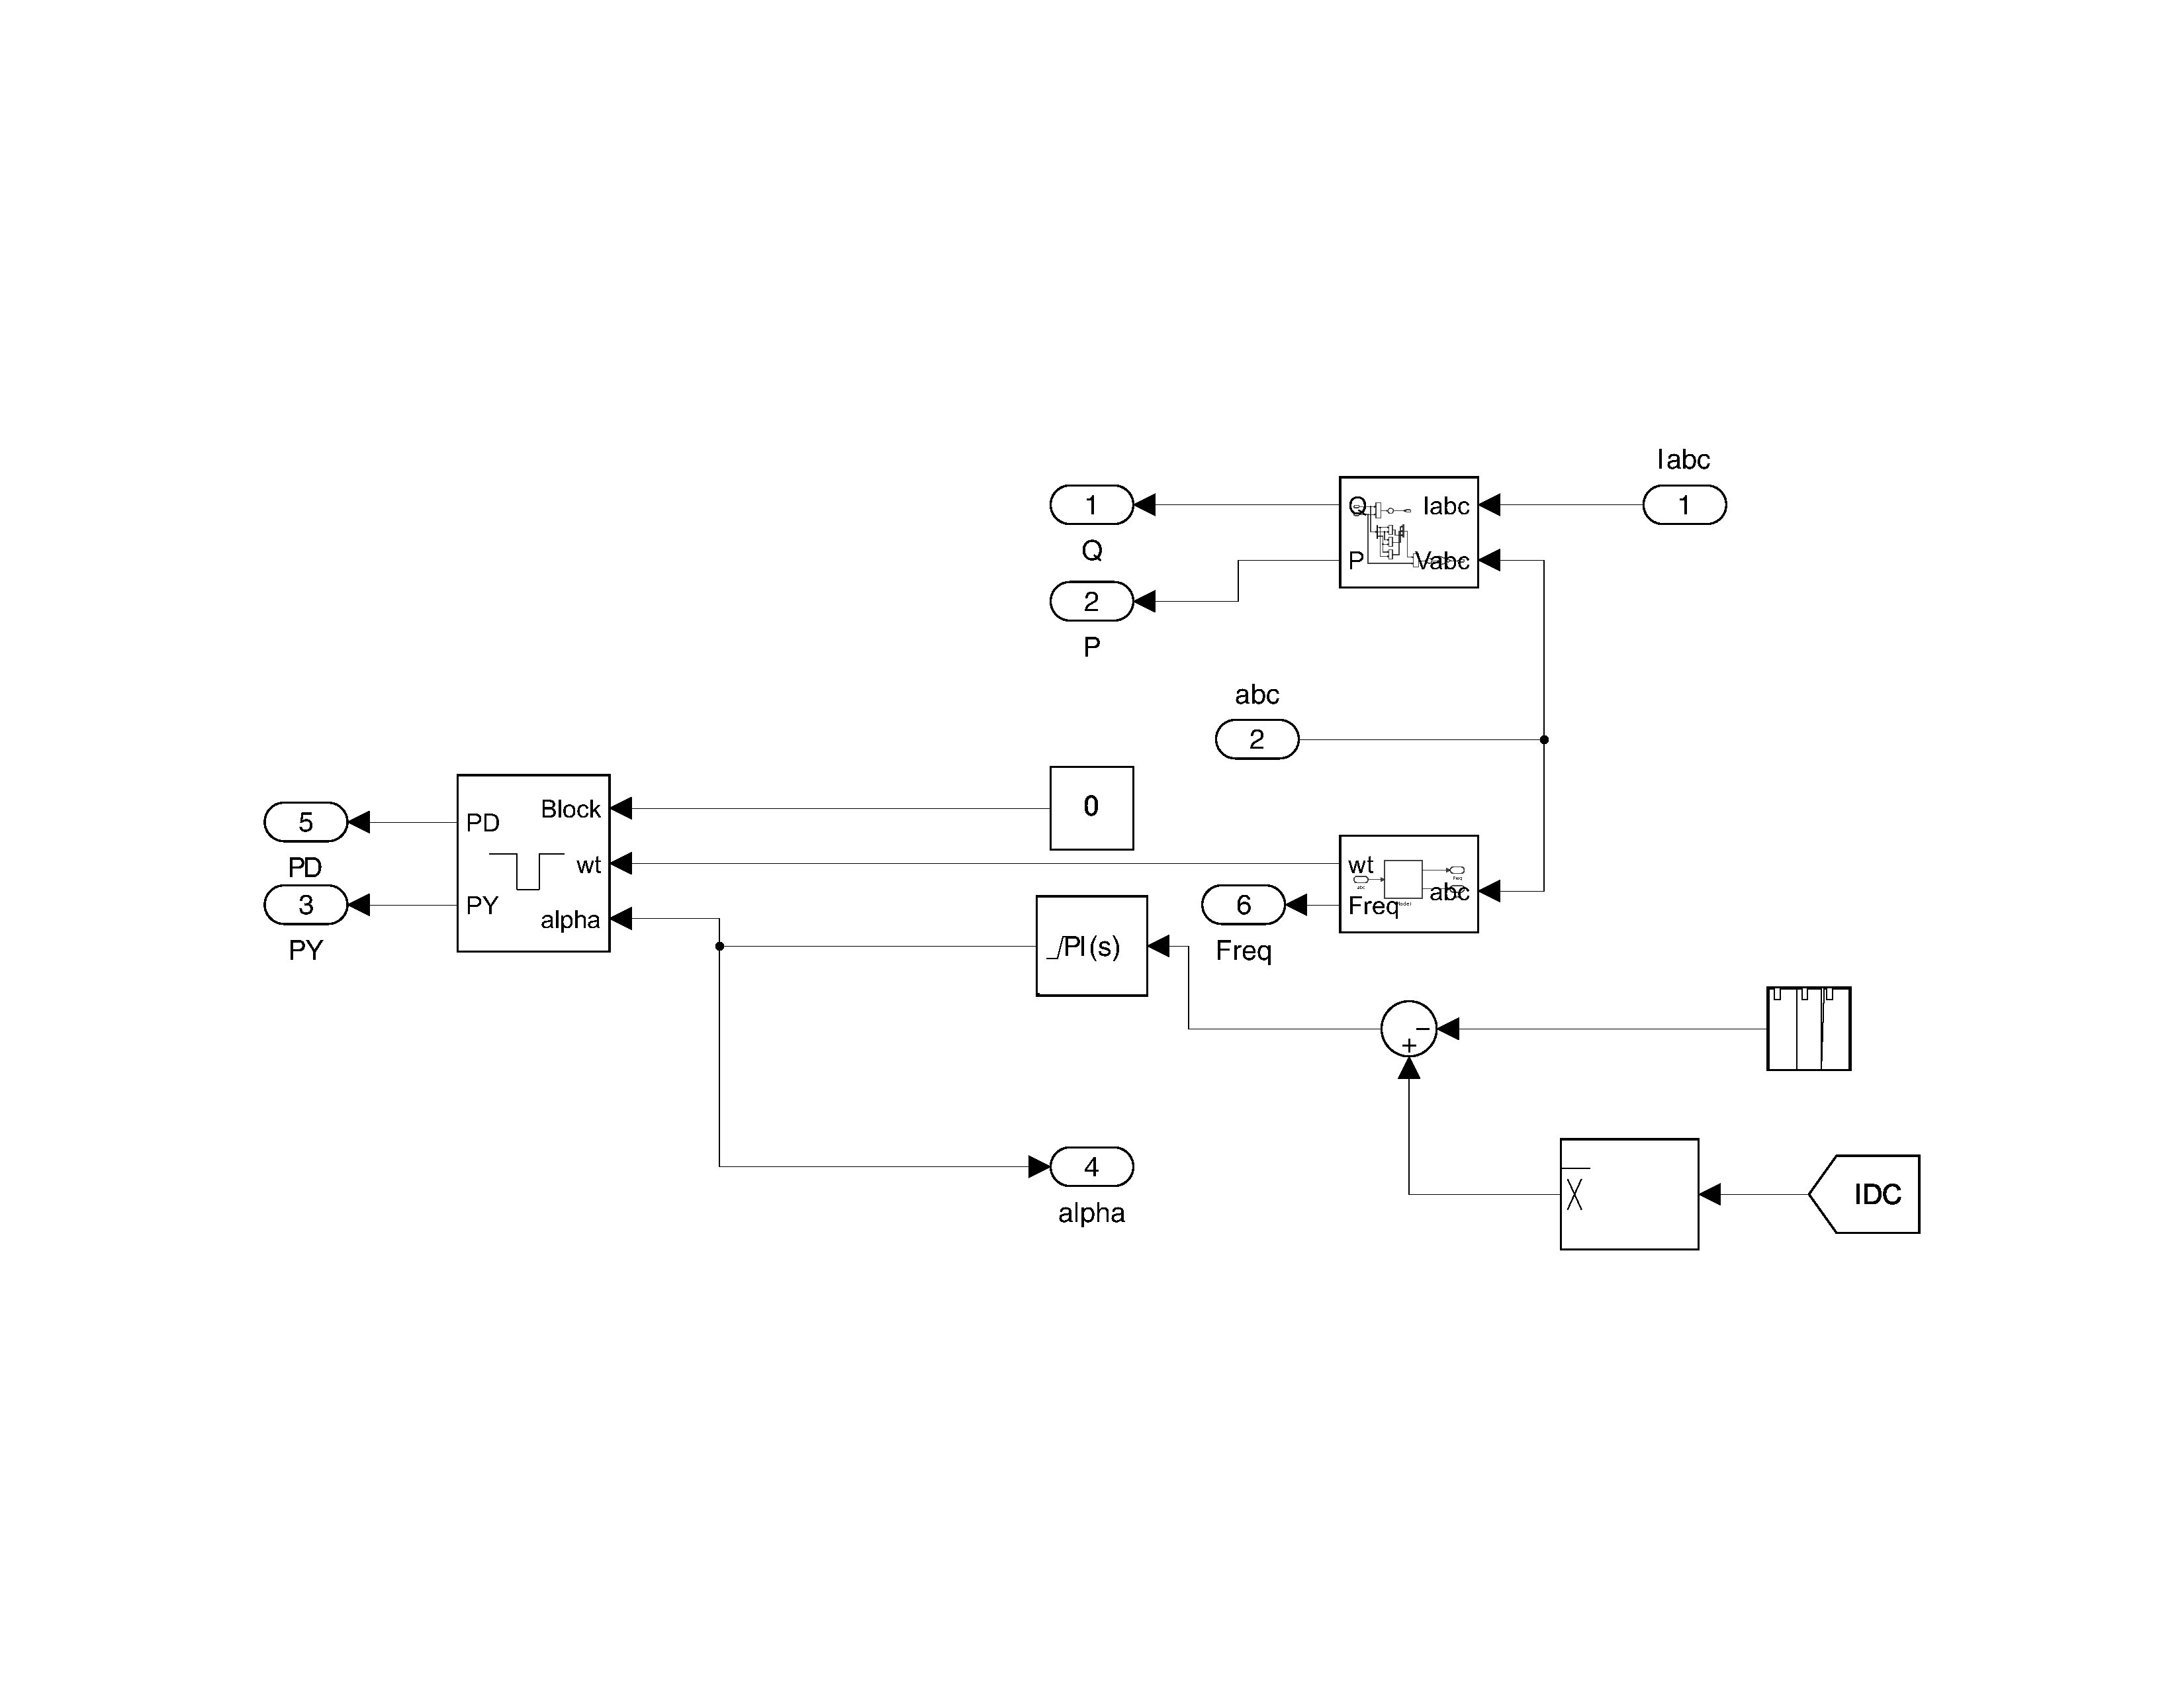
\includegraphics[width=\textwidth]{B_sys3.jpg}
        \caption{\textbf{Receiving Control Circuit:} Includes IDC measurement.}
    \end{subfigure}
    \hfill
    \begin{subfigure}{0.48\textwidth}
        \centering
        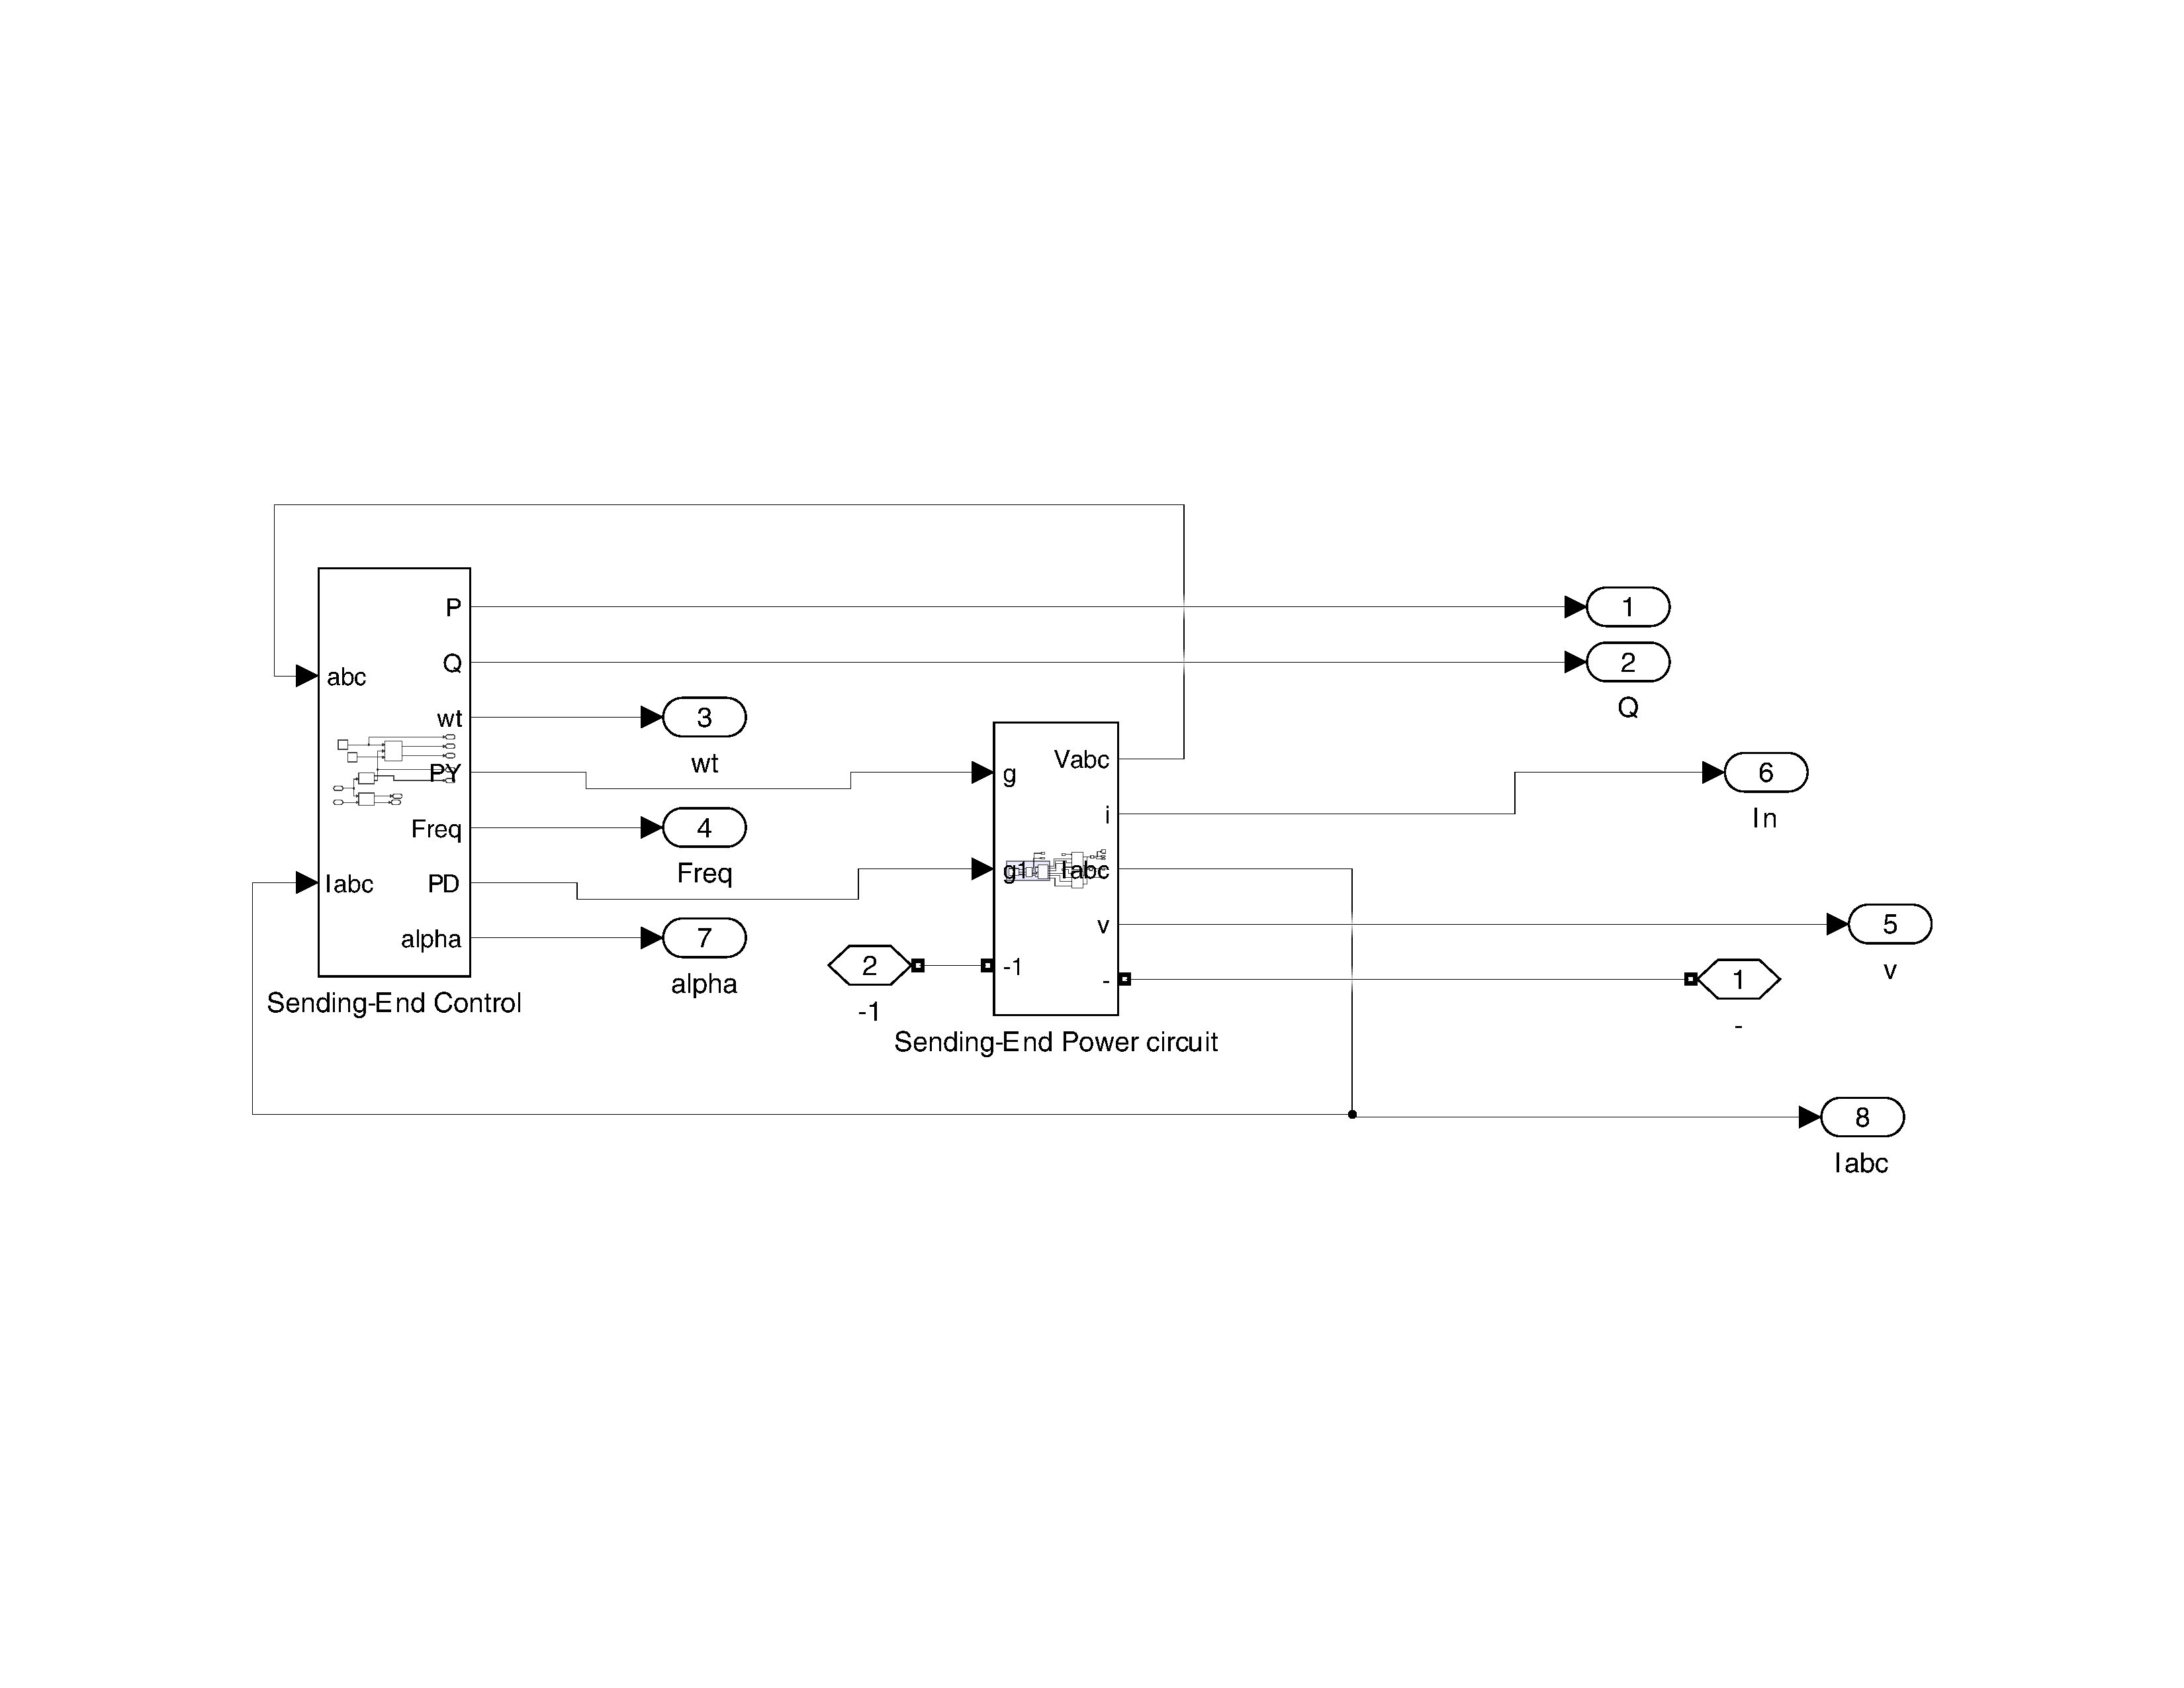
\includegraphics[width=\textwidth]{B_sys4.jpg}
        \caption{\textbf{Sending Control Circuit:}}
    \end{subfigure}
    
    \vspace{0.3cm}
    \begin{subfigure}{0.48\textwidth}
        \centering
        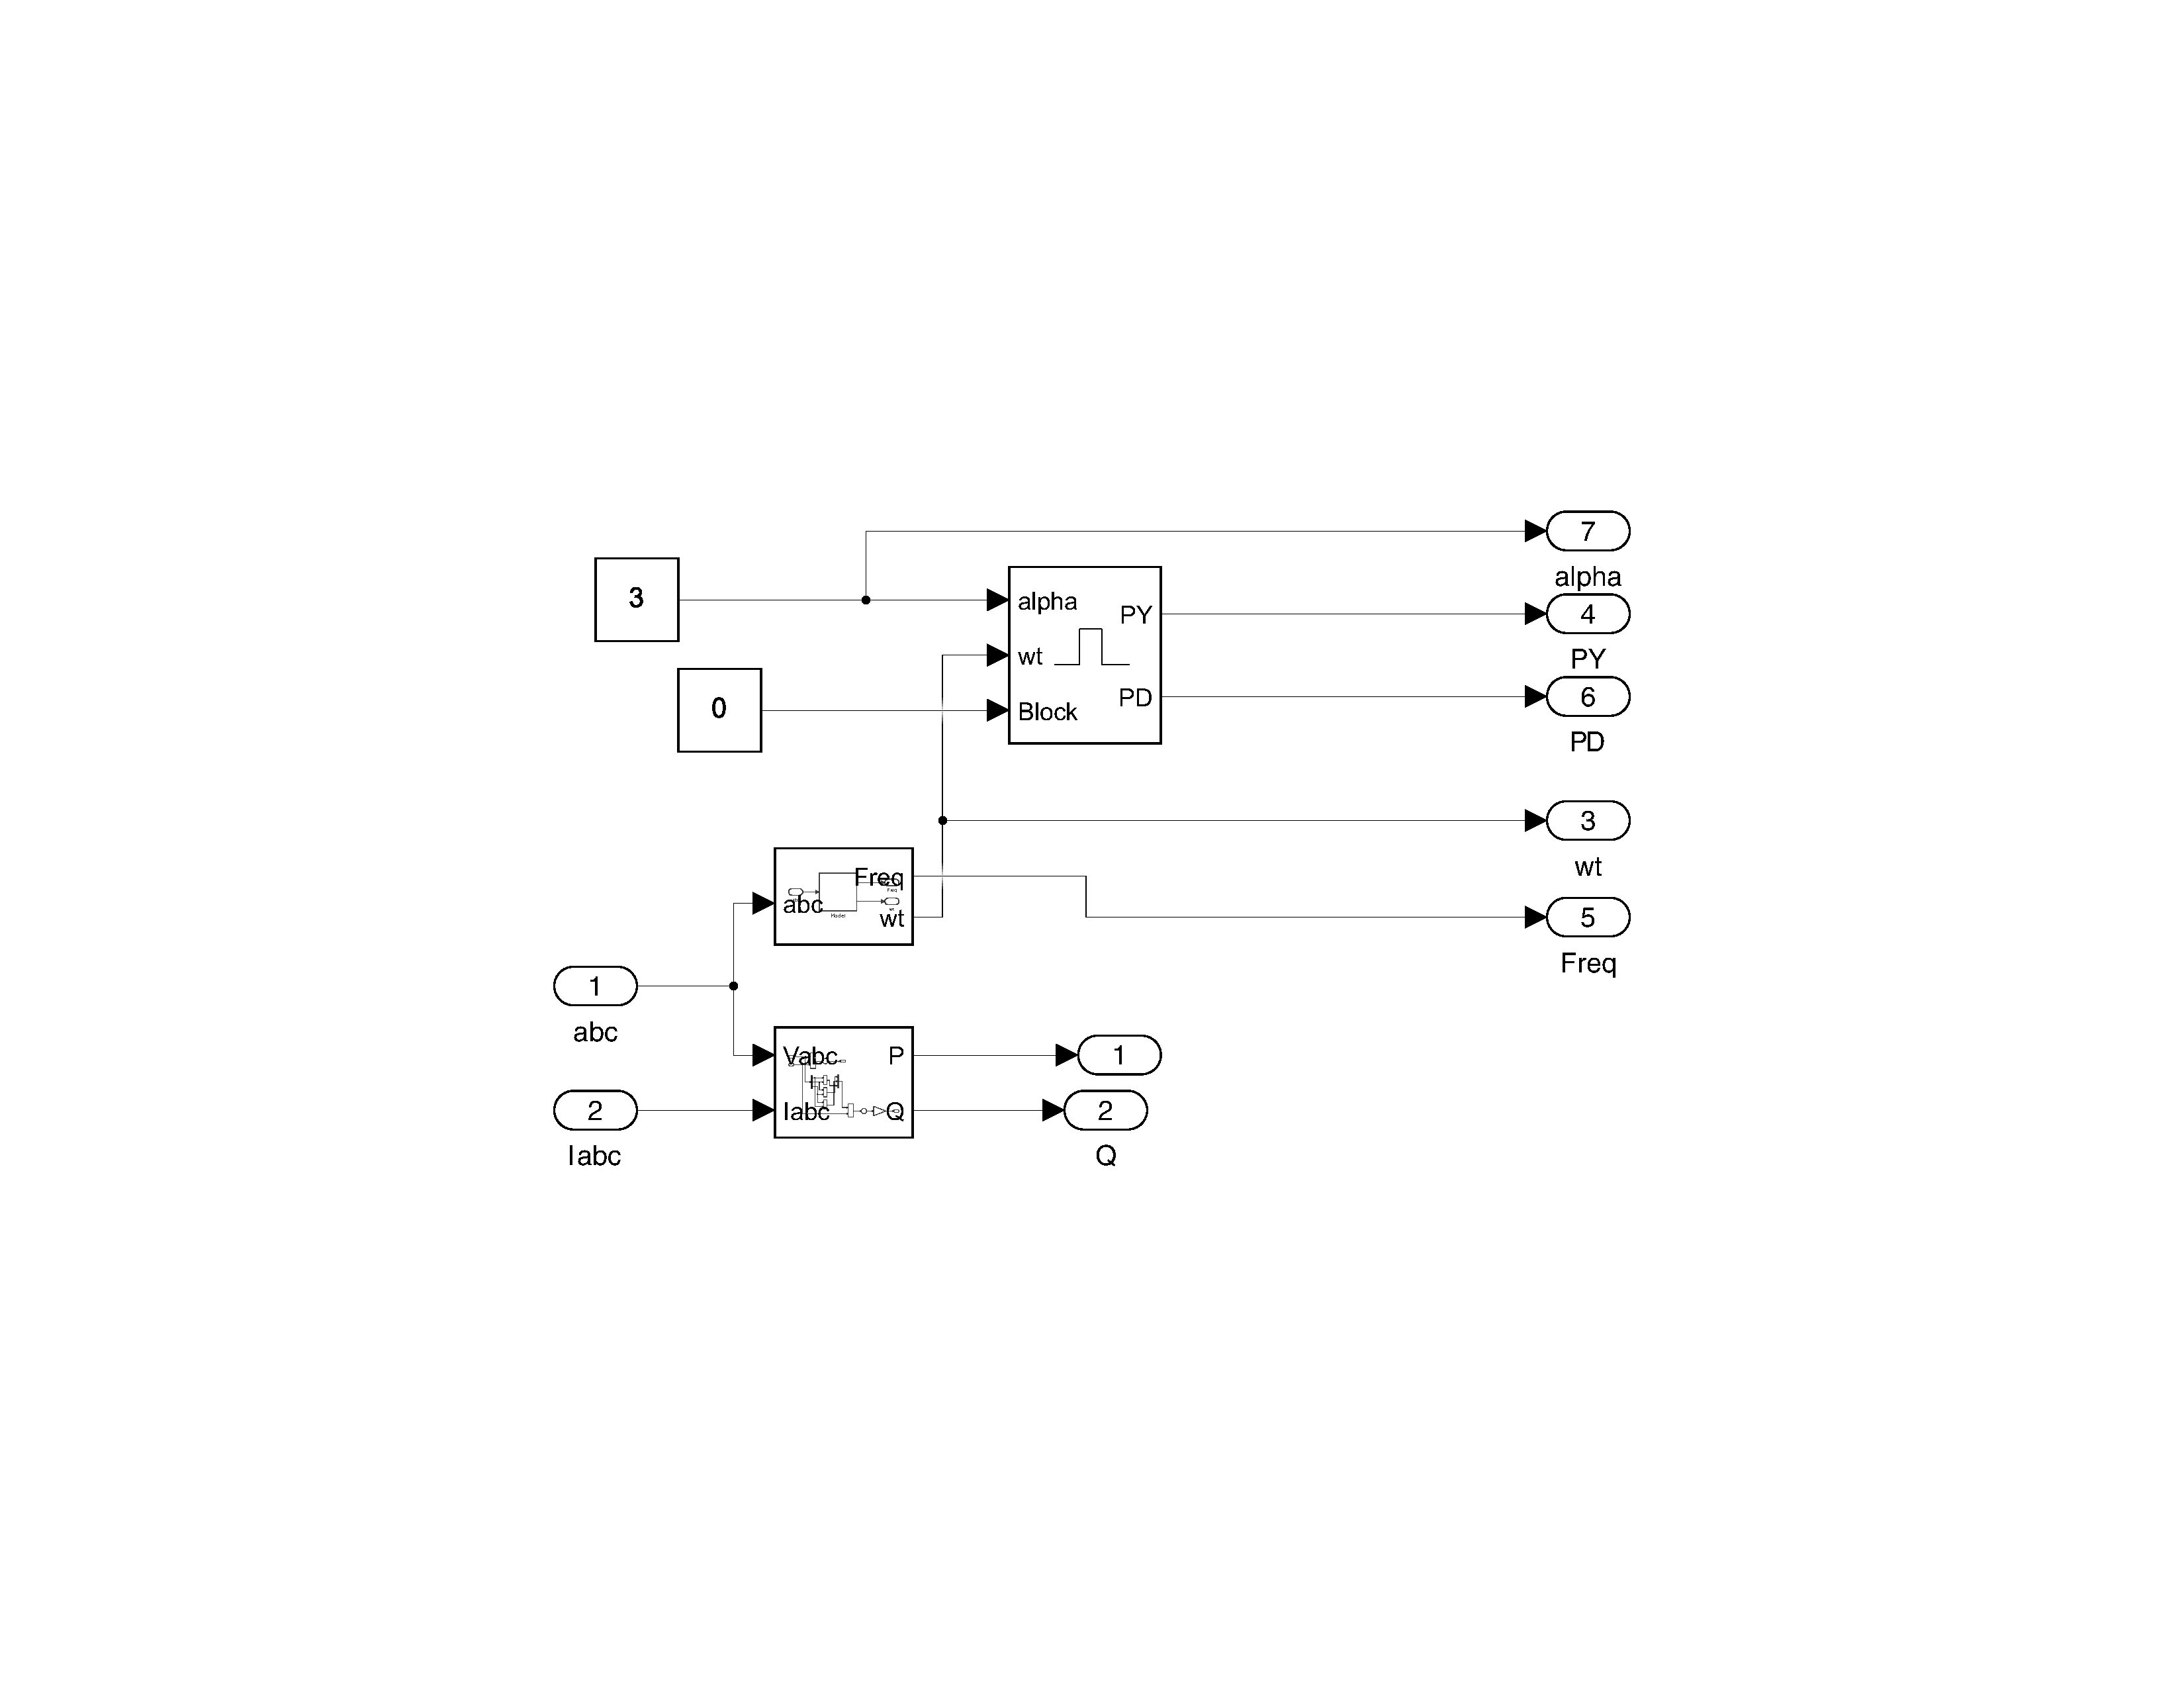
\includegraphics[width=\textwidth]{B_sys5.jpg}
        \caption{\textbf{Pulse Generator Unit:}}
    \end{subfigure}
    \hfill
    \begin{subfigure}{0.48\textwidth}
        \centering
        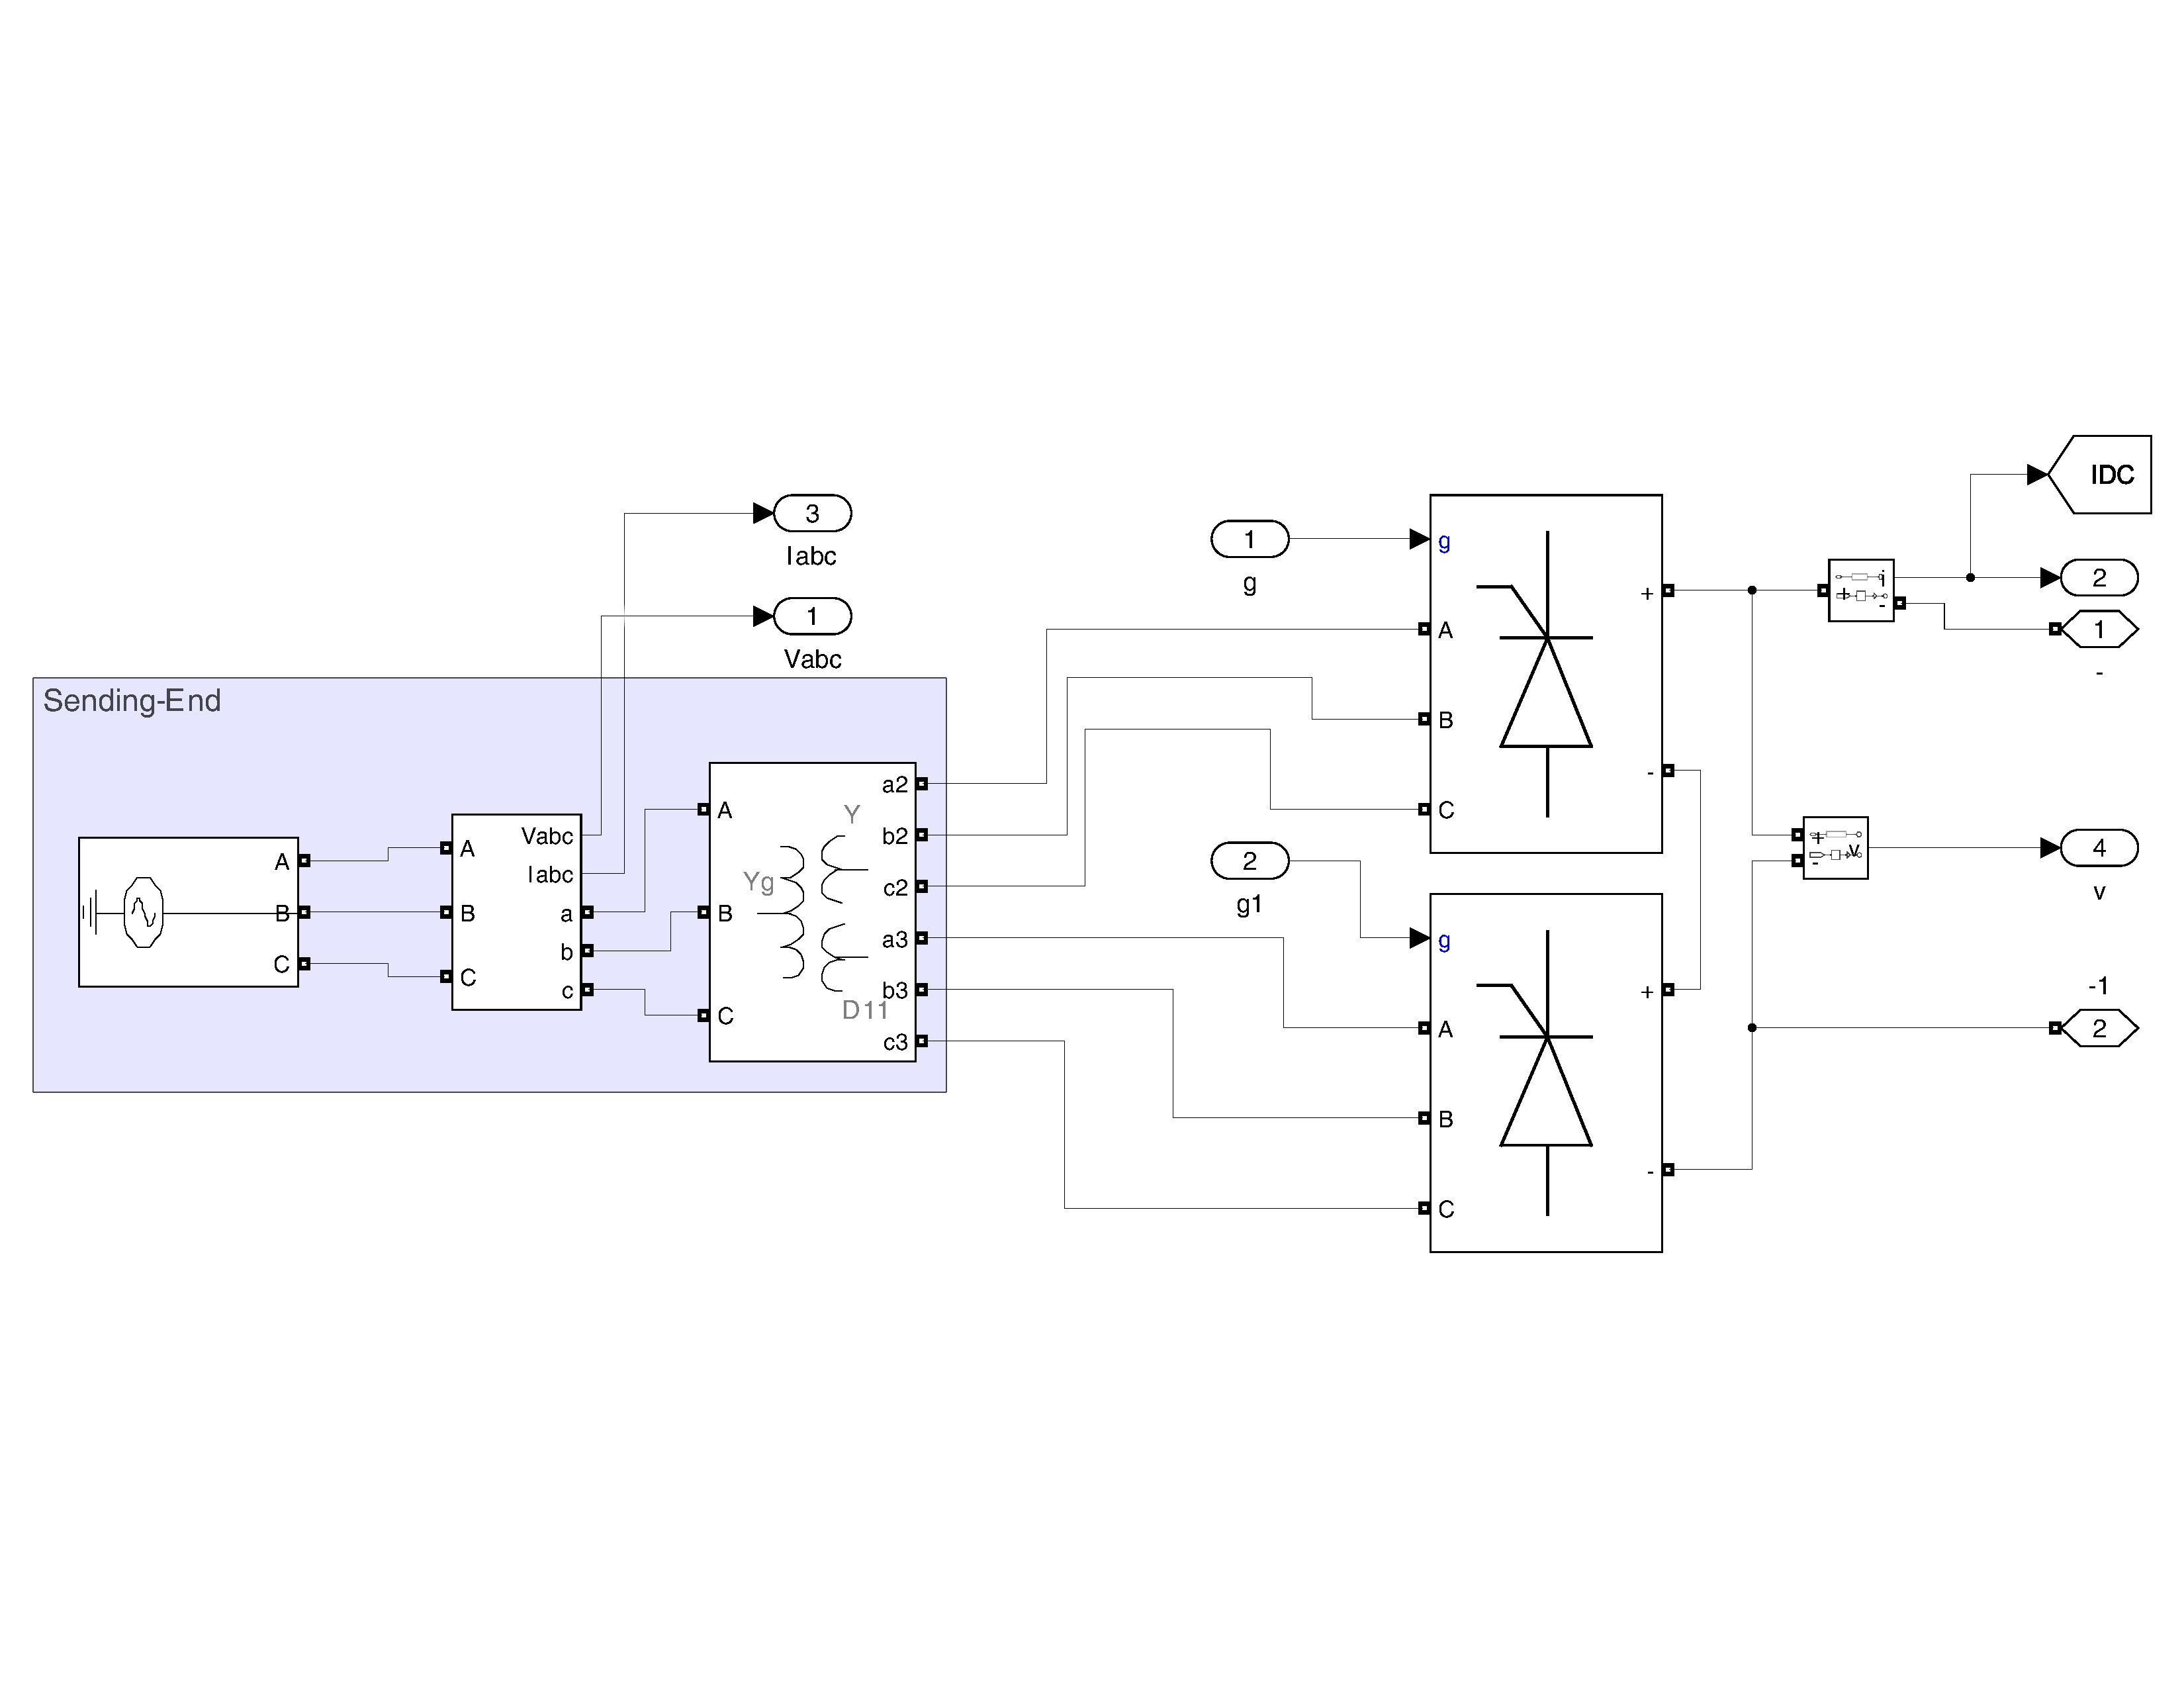
\includegraphics[width=\textwidth]{B_sys6.jpg}
        \caption{\textbf{Sending Power Circuit:} Emitting the IDC signal.}
    \end{subfigure}
    \caption{Subsystem Configurations modified for Case B.}
\end{figure}

\newpage
\subsection{Overall System Performance (Case B)}
Figures 13 and 14 demonstrate the successful control handover during the 25\% voltage sag.

\begin{figure}[H]
    \centering
    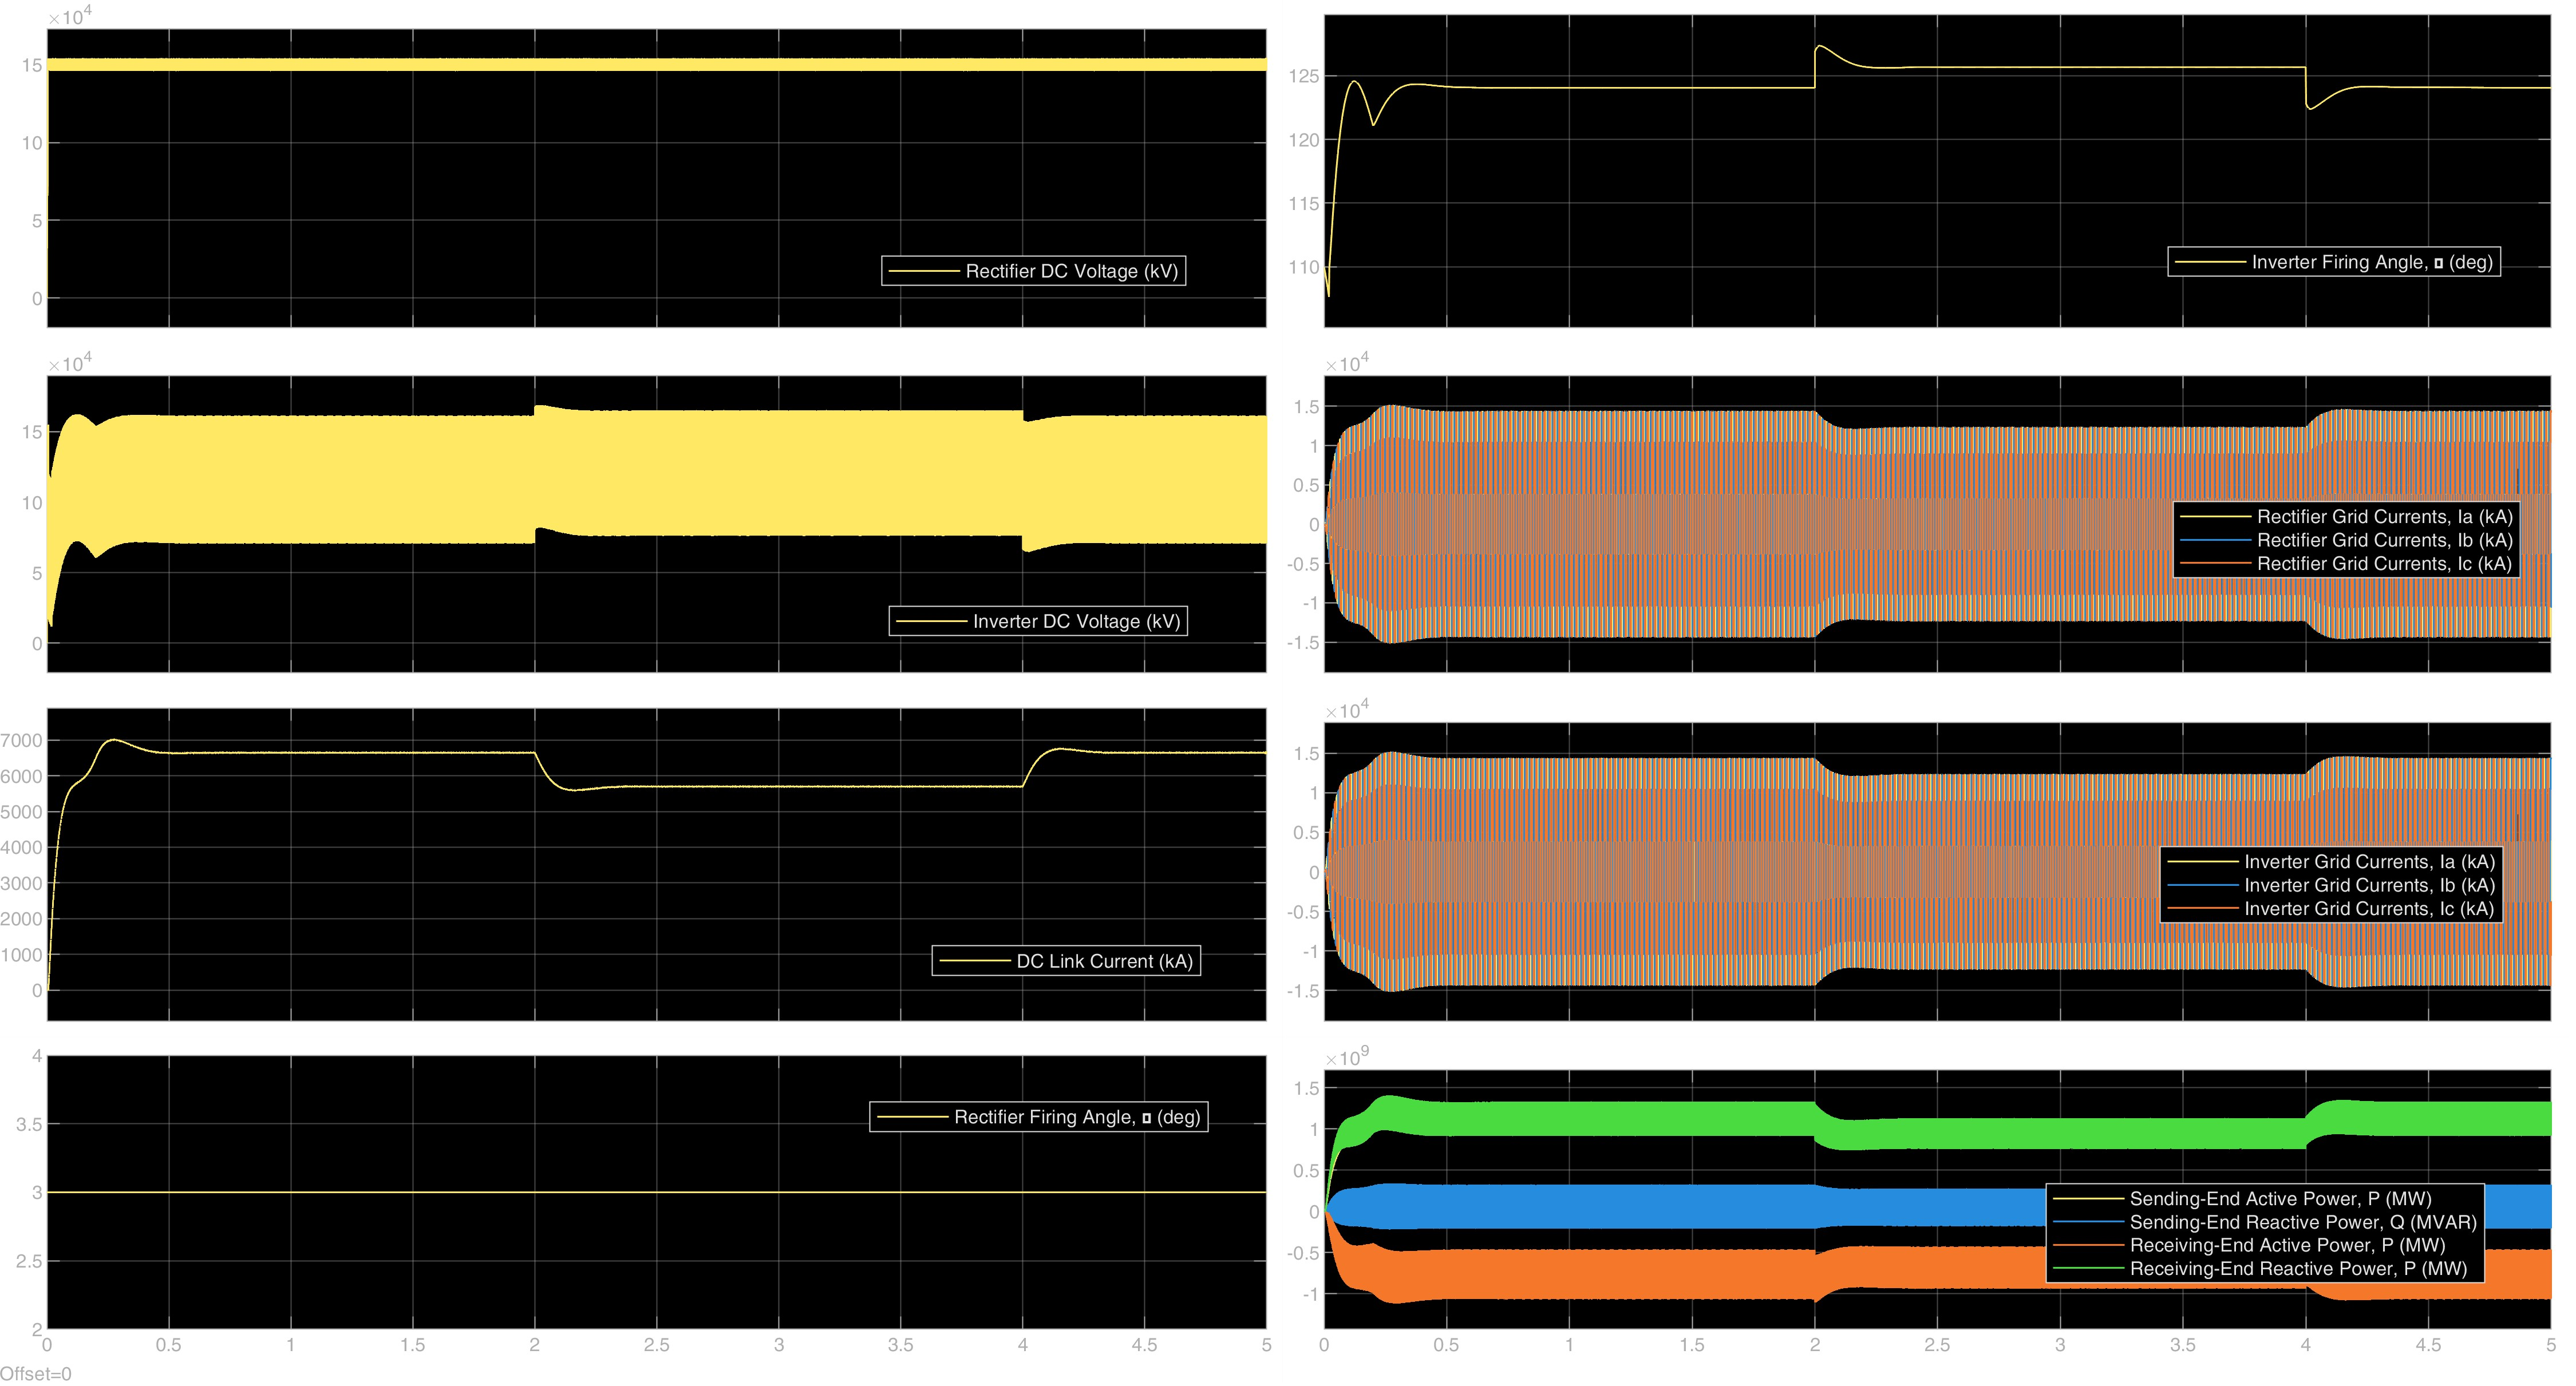
\includegraphics[width=0.95\textwidth]{B_VI.jpg}
    \caption{\textbf{VI Scope:} Highlights the critical transition point where the inverter abandons CEA mode and successfully takes over the Constant Current (CC) regulation.}
\end{figure}

\begin{figure}[H]
    \centering
    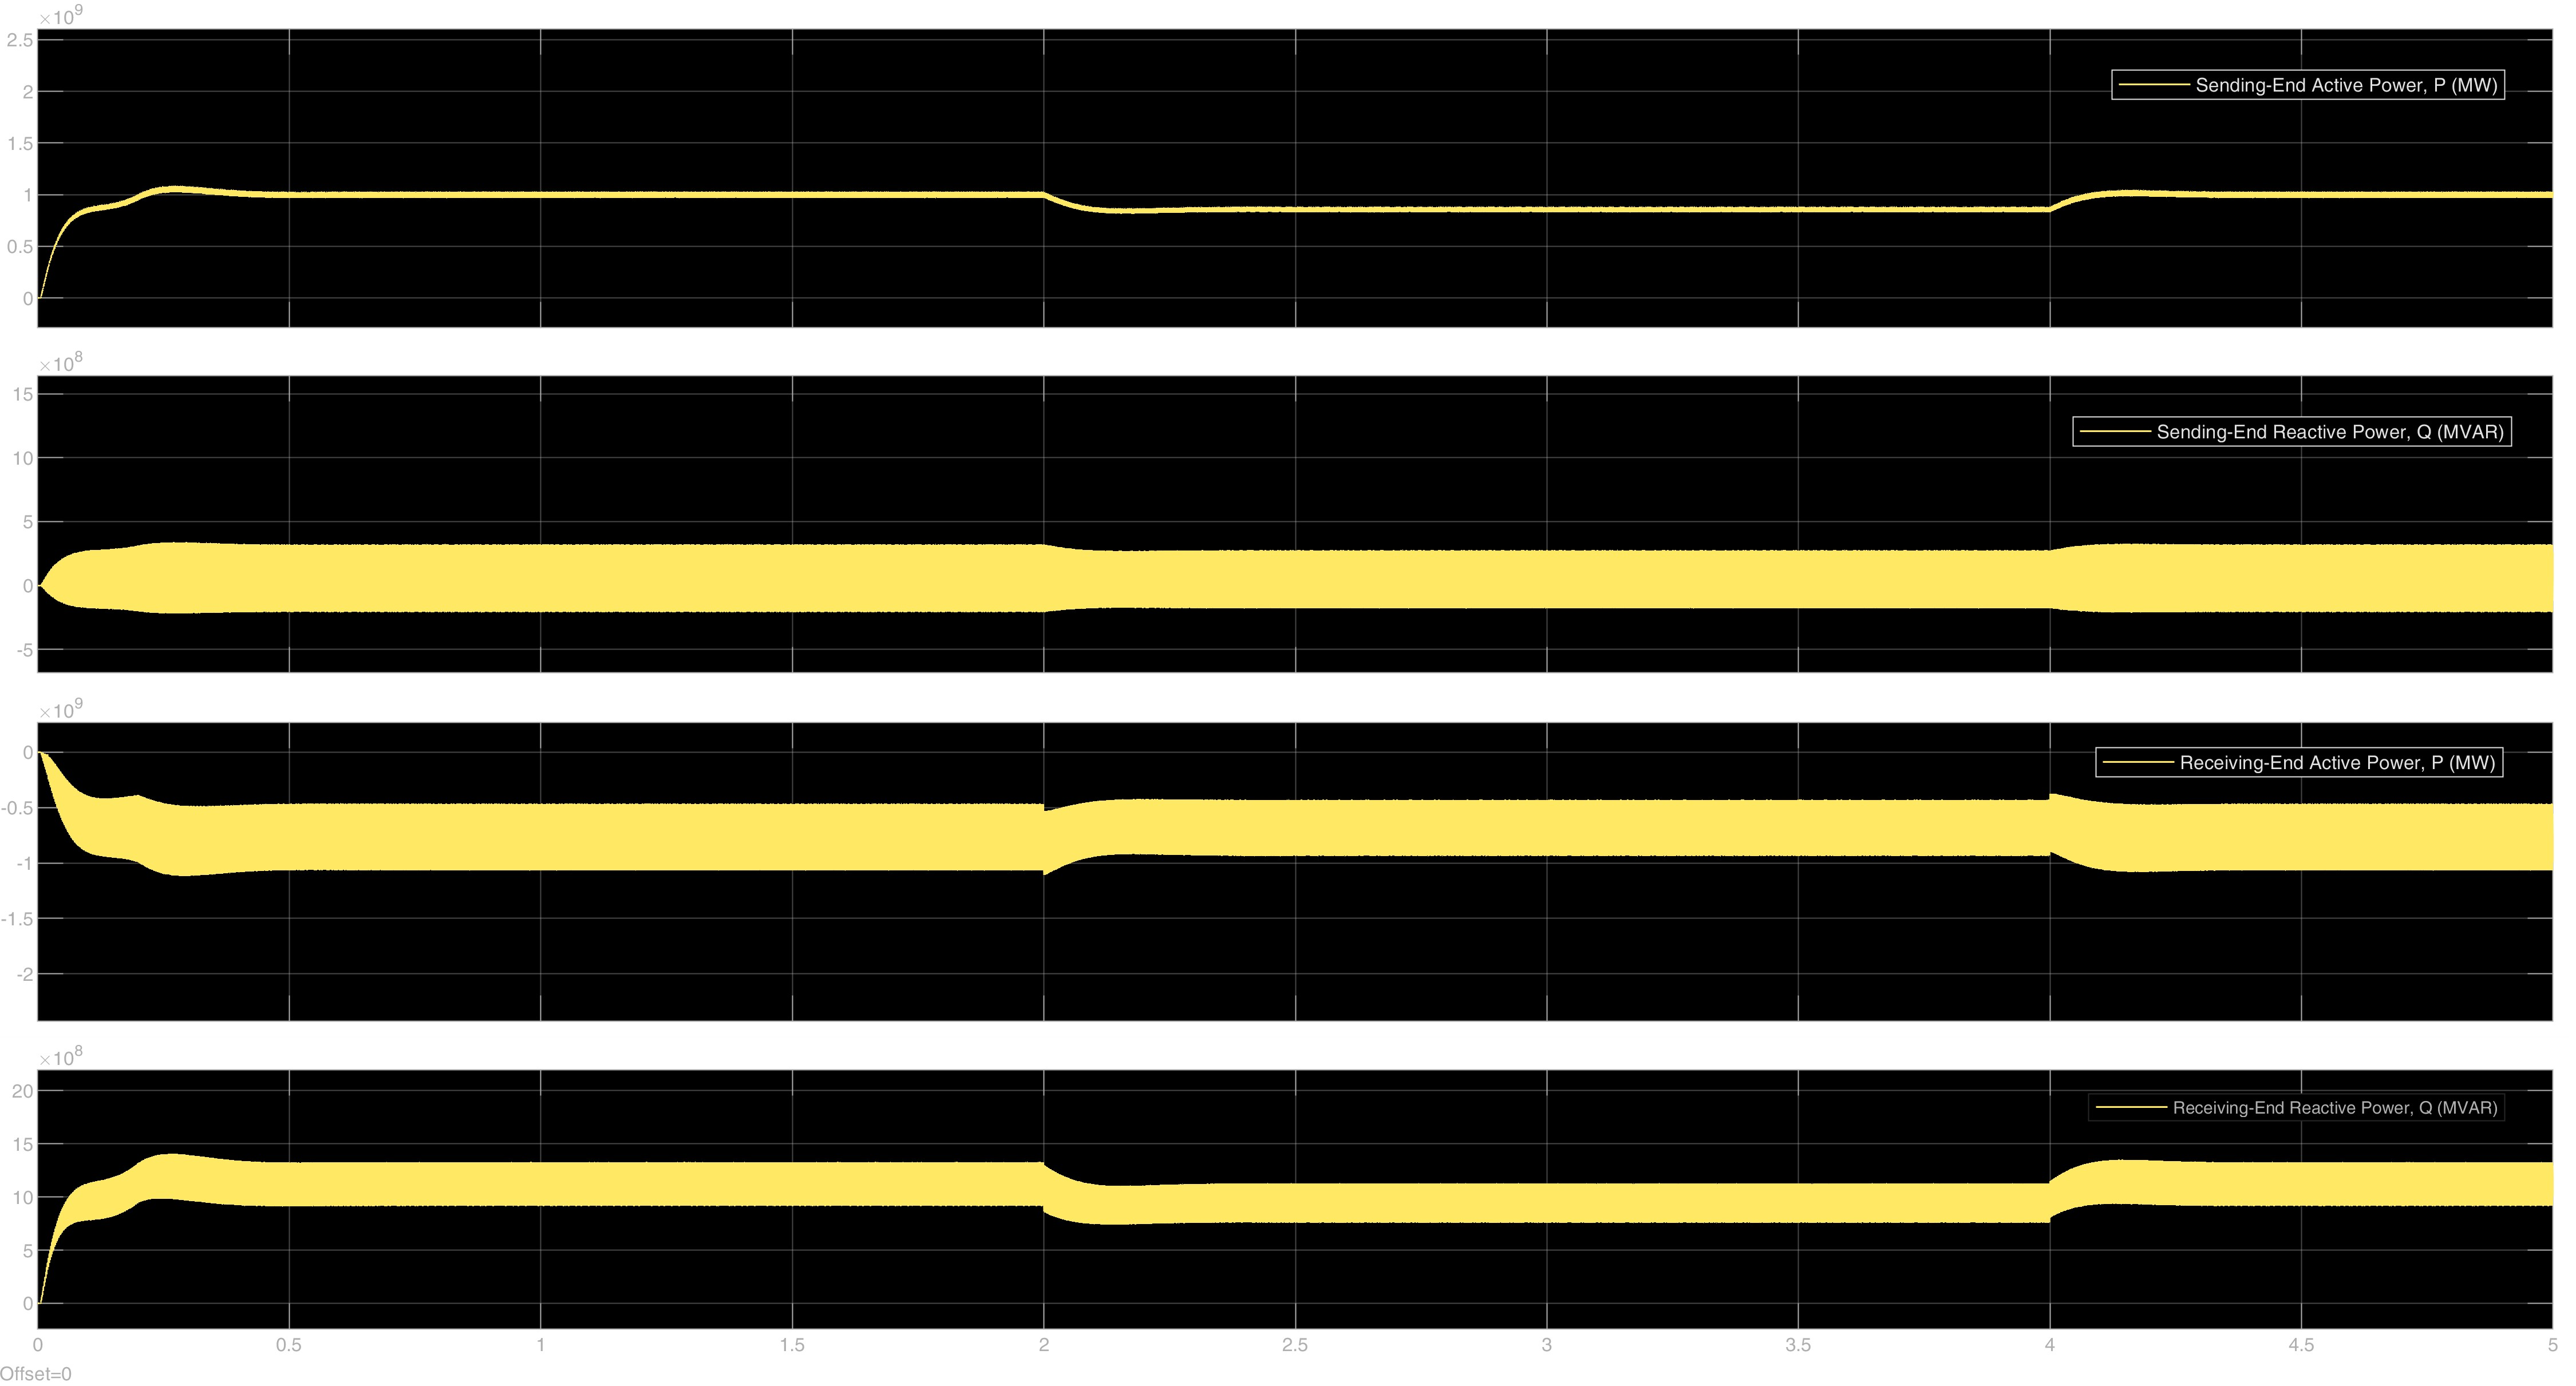
\includegraphics[width=0.95\textwidth]{B_Power.jpg}
    \caption{\textbf{Powers Scope:} Shows the resulting active and reactive power transfer limitations dictated by the severe voltage sag on the sending end.}
\end{figure}

\newpage
\subsection{Detailed Waveform Analysis}

\begin{figure}[H]
    \centering
    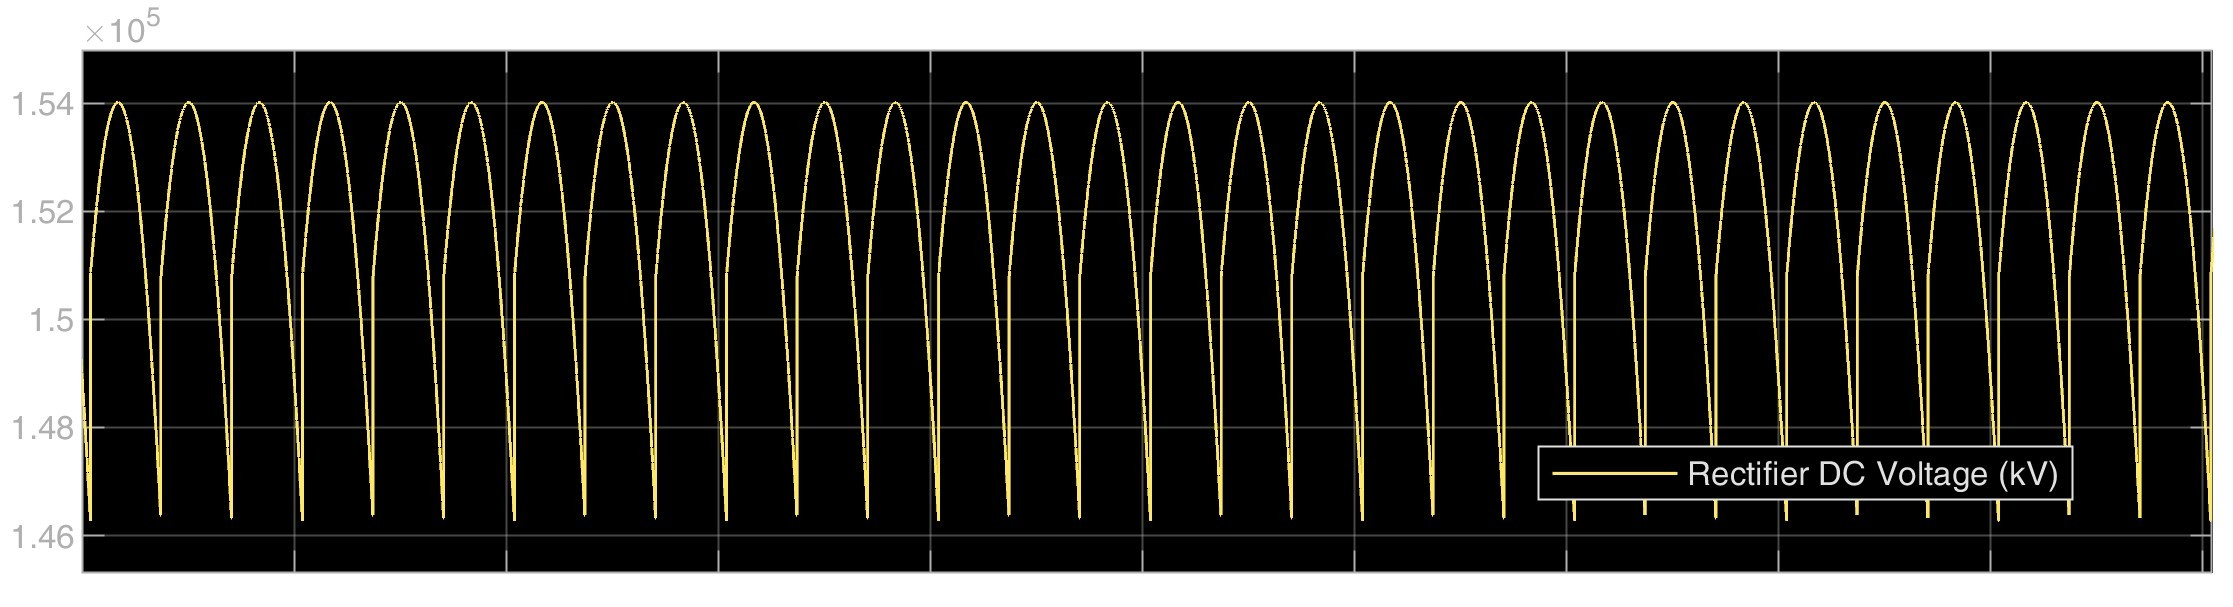
\includegraphics[width=0.75\textwidth]{B_1.jpg}
    \caption{\textbf{Rectifier DC Voltage ($V_{rect}$)}}
\end{figure}
A clear and sustained drop in the DC voltage (falling to approximately 150 kV) is observed. This is the direct physical consequence of the 25\% AC voltage sag applied to the sending-end source, fundamentally reducing the maximum achievable DC output capability of the rectifier bridge.

\vspace{0.5cm}
\begin{figure}[H]
    \centering
    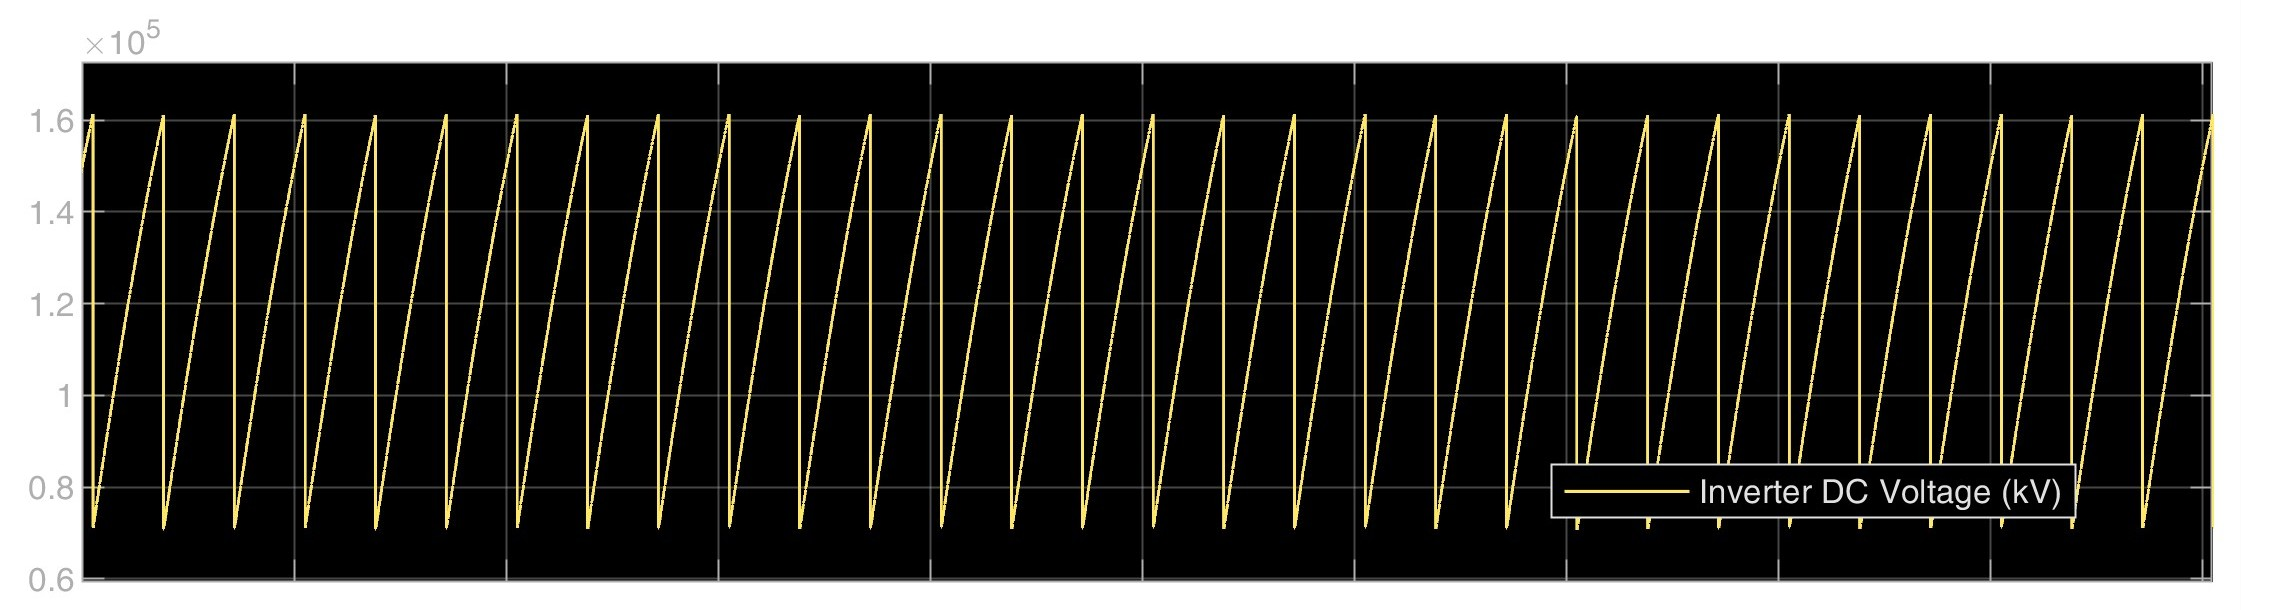
\includegraphics[width=0.75\textwidth]{B_2.jpg}
    \caption{\textbf{Inverter DC Voltage ($V_{inv}$)}}
\end{figure}
To maintain the flow of current against the collapsed rectifier voltage, the inverter dynamically reduces the magnitude of its opposing back-EMF. By adjusting its voltage downwards, the inverter guarantees that the forward potential difference ($\Delta V$) remains positive and sufficient to drive the margin-adjusted current.

\vspace{0.5cm}
\begin{figure}[H]
    \centering
    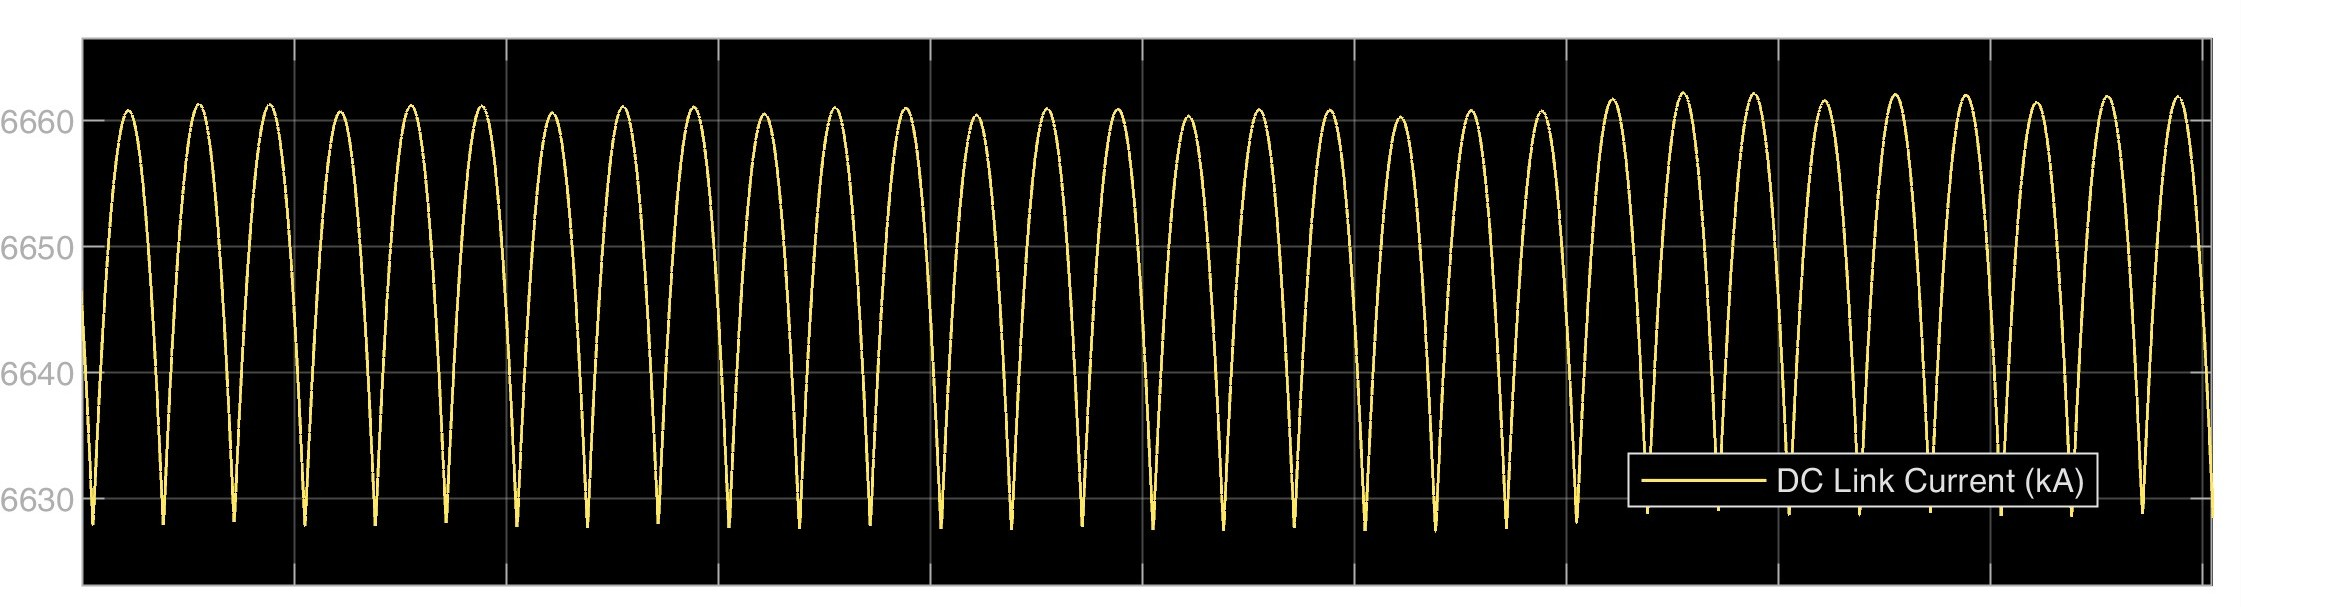
\includegraphics[width=0.75\textwidth]{B_3.jpg}
    \caption{\textbf{DC Link Current ($I_{dc}$)}}
\end{figure}
Despite the severe fault, the DC current does not collapse. It smoothly transitions to track the new, lower reference points established by the 5\% current margin (e.g., adjusting from 7000 A down to 6650 A). This waveform serves as definitive proof that the inverter's CC controller has successfully assumed command of the link.

\vspace{0.5cm}
\begin{figure}[H]
    \centering
    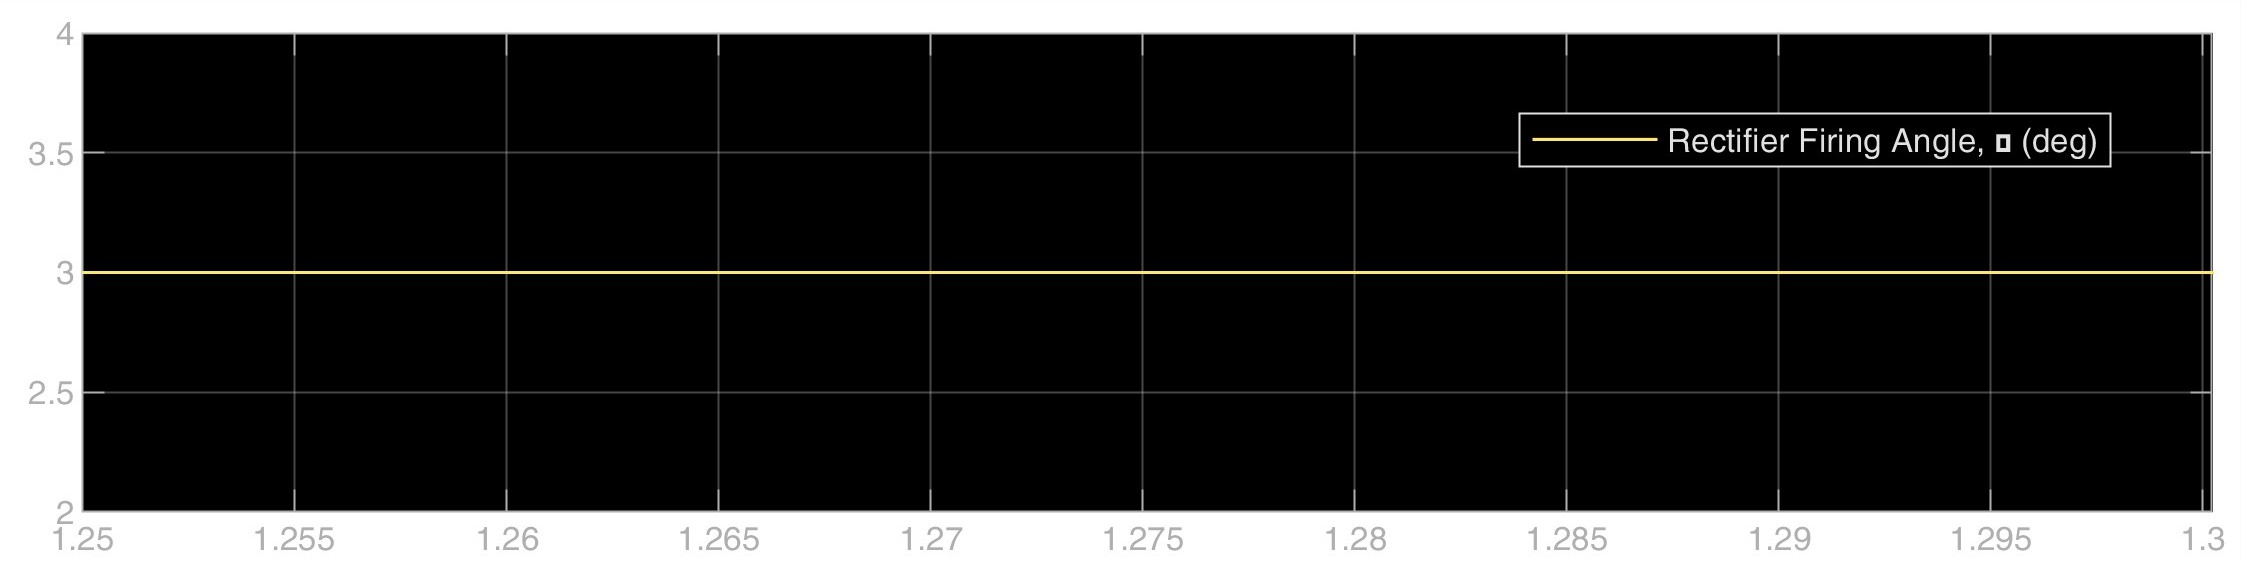
\includegraphics[width=0.75\textwidth]{B_4.jpg}
    \caption{\textbf{Rectifier Firing Angle ($\alpha_{rect}$)}}
\end{figure}
The rectifier's PI controller integrates to its absolute minimum in a futile attempt to raise the voltage, causing the firing angle to saturate and flatline at $\alpha_{min} = 3^{\circ}$. The rectifier is now effectively operating as an uncontrolled diode bridge (Constant Ignition Angle - CIA mode) to squeeze out the maximum possible voltage.

\vspace{0.5cm}
\begin{figure}[H]
    \centering
    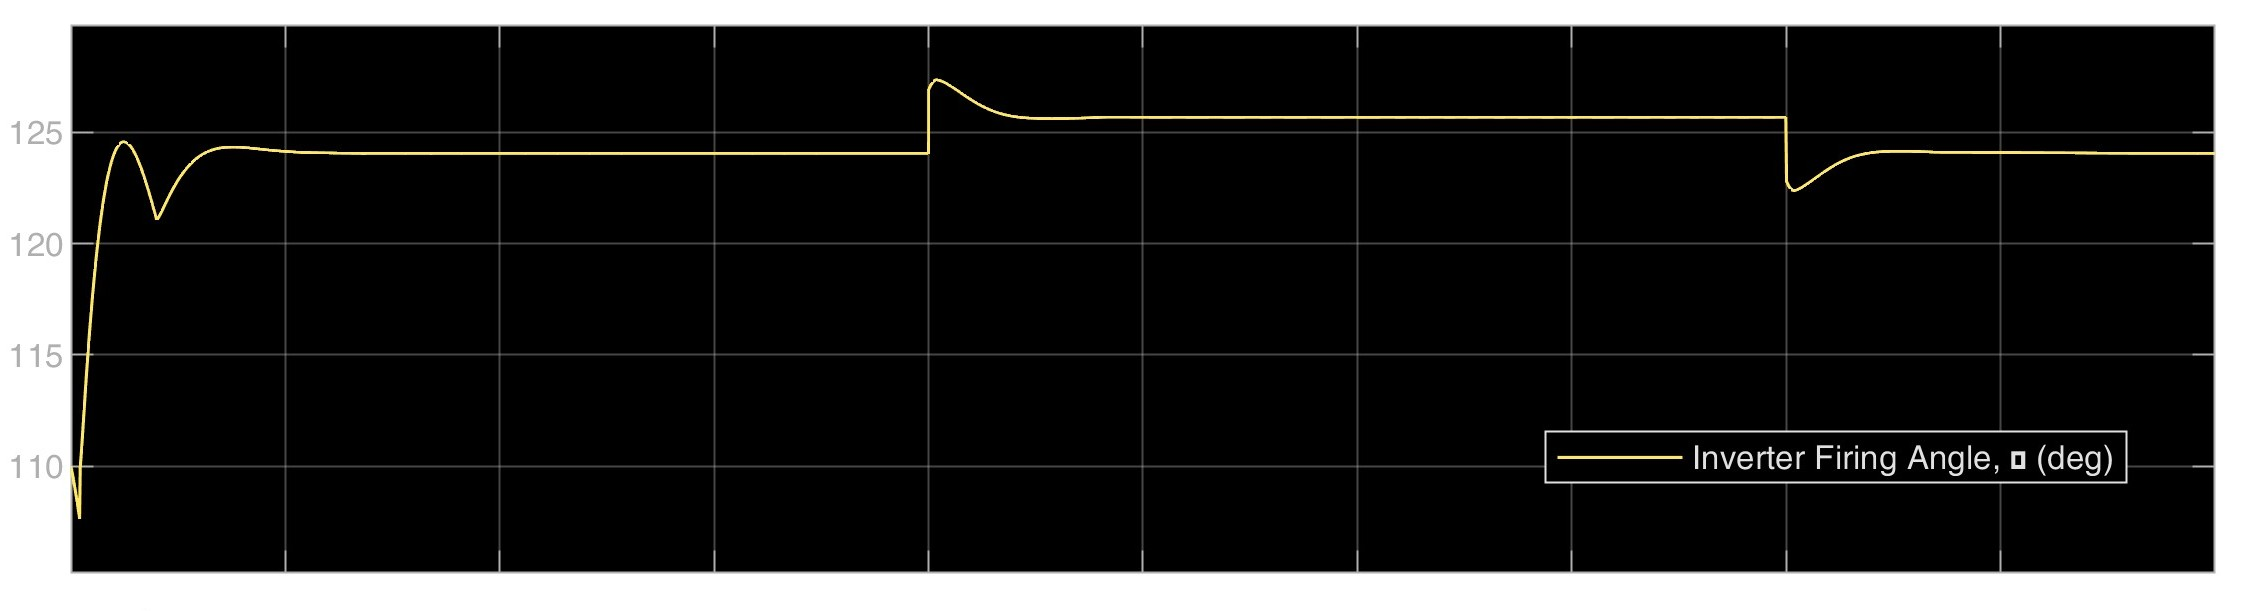
\includegraphics[width=0.75\textwidth]{B_5.jpg}
    \caption{\textbf{Inverter Firing Angle ($\alpha_{inv}$)}}
\end{figure}
In stark contrast to Case A, the inverter firing angle is no longer fixed at a safe margin. The inverter abandons CEA mode and actively modulates $\alpha_{inv}$ to regulate the DC line current, proving the operational execution of the fallback CC control loop.

\vspace{0.5cm}
\begin{figure}[H]
    \centering
    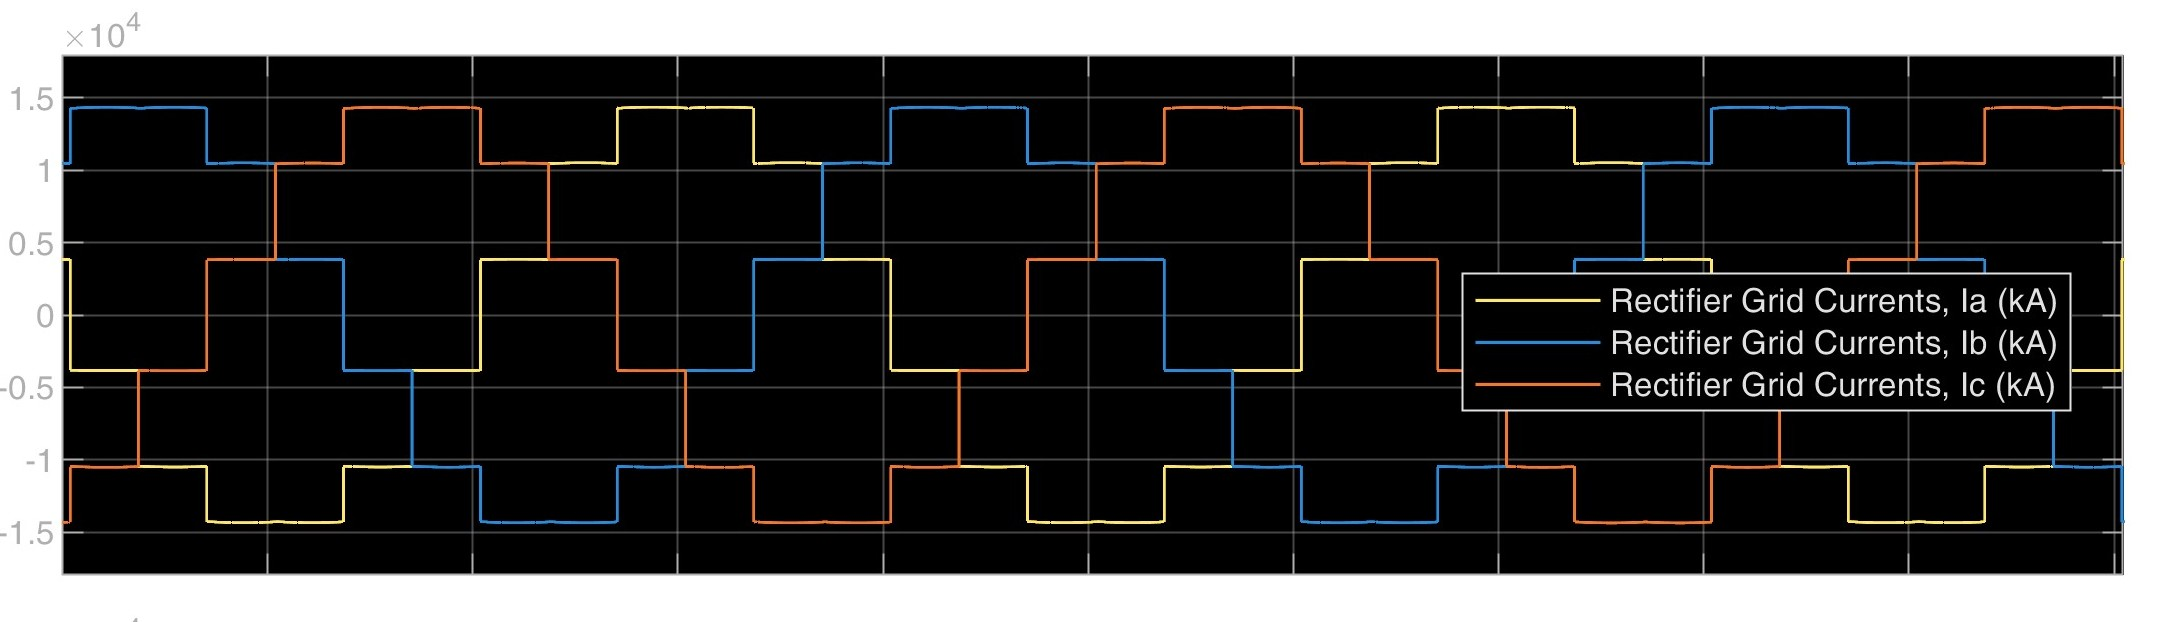
\includegraphics[width=0.75\textwidth]{B_6.jpg}
    \caption{\textbf{Rectifier Grid Currents}}
\end{figure}
While the quasi-square shape of the currents remains intact, their overall magnitudes are visibly reduced. This reduction perfectly corresponds to the newly enforced 5\% margin drop in the DC link current caused by the control handover.

\vspace{0.5cm}
\begin{figure}[H]
    \centering
    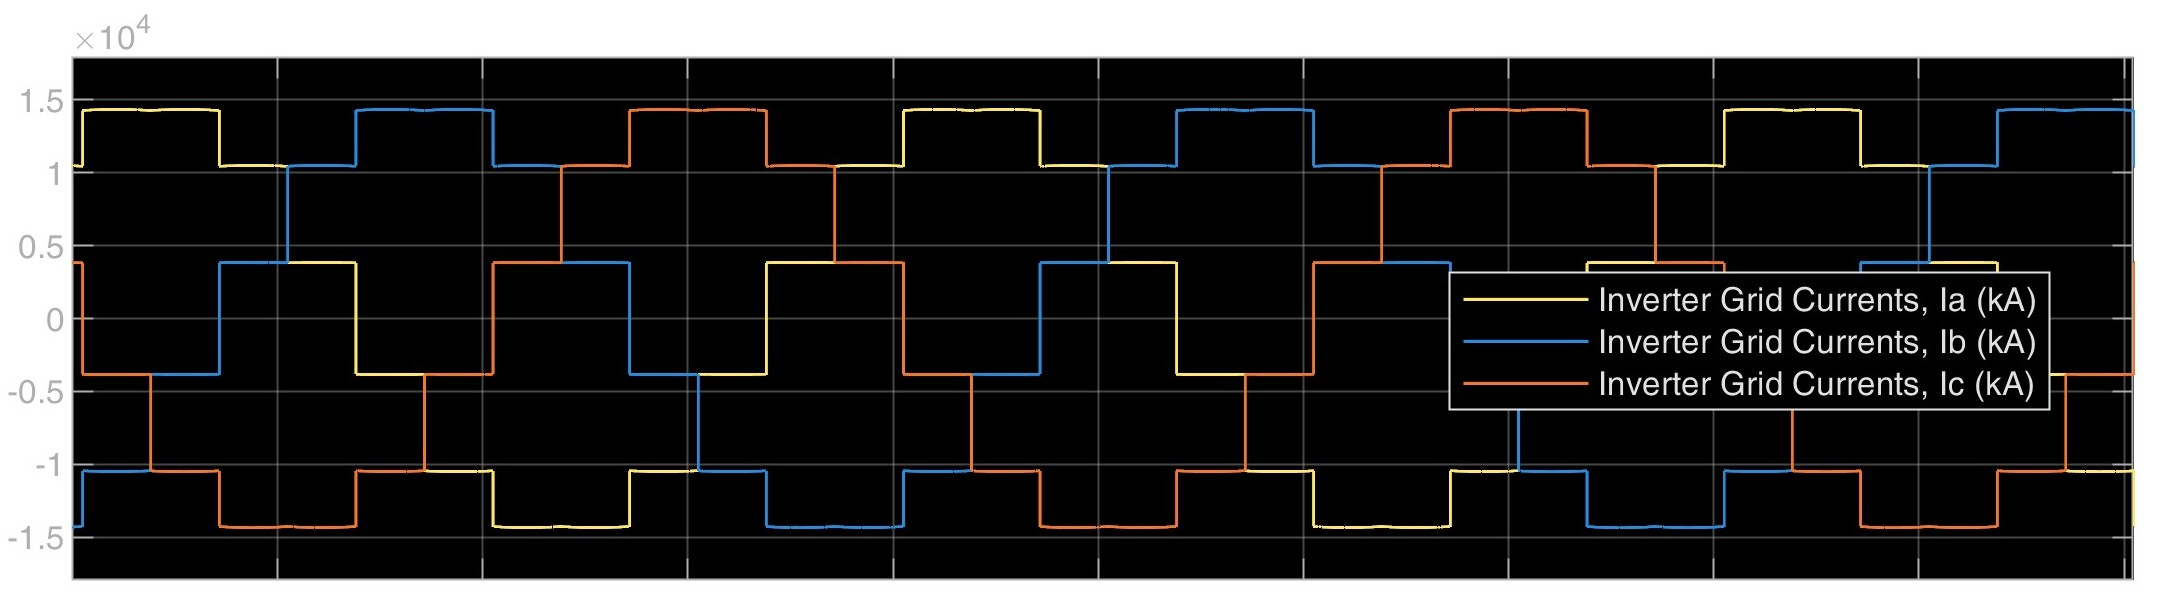
\includegraphics[width=0.75\textwidth]{B_7.jpg}
    \caption{\textbf{Inverter Grid Currents}}
\end{figure}
The AC currents injected into the receiving grid accurately mirror the new current margins. The ability of the inverter to continue supplying stable, balanced, and low-harmonic AC currents during a severe sending-end fault demonstrates excellent fault-ride-through capability.

\vspace{0.5cm}
\begin{figure}[H]
    \centering
    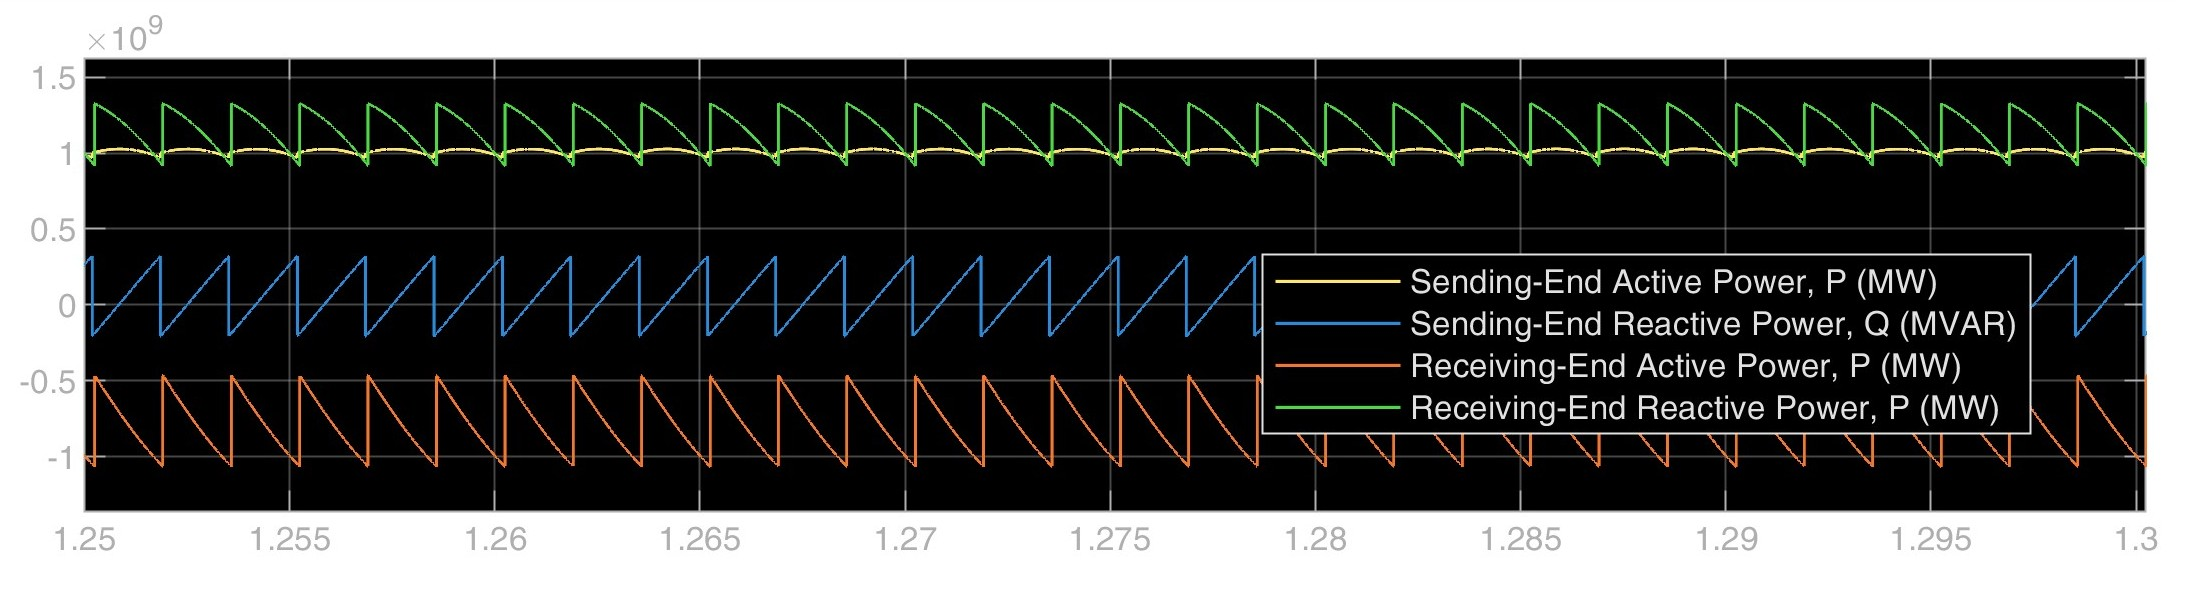
\includegraphics[width=0.75\textwidth]{B_8.jpg}
    \caption{\textbf{Active and Reactive Power ($P \& Q$)}}
\end{figure}
Due to the significant loss of DC voltage, the overall active power ($P$) transfer capacity is inherently reduced. Simultaneously, the reactive power ($Q$) demand shifts drastically due to the new extreme firing angles, highlighting the profound impact grid faults have on converter efficiency and MVAR requirements.

\section{Conclusion}
The comprehensive simulation of the 12-pulse HVDC transmission system successfully validates its steady-state precision and dynamic resilience. Under normal conditions, the primary CC/CEA control strategy ensures fast, accurate, and stable power transfer. Crucially, during the severe AC voltage sag, the system demonstrated exceptional fault tolerance. The coordinated control handover—where the rectifier saturated into CIA mode and the inverter seamlessly adopted CC mode using a 5\% current margin—prevented a catastrophic collapse of the DC link. The results emphasize the critical importance of advanced, adaptive control logic in maintaining power continuity and ensuring the stability of modern power electronics networks.

\end{document}